% !TEX TS-program = pdflatex
% !TEX root = ../LightMicroRep.tex

%************************************************
\chapter{Microphotography}
\label{chp:Microphotography}
%************************************************
\numberwithin{figure}{section}
%----------------------------------------------------------------------------------------
%	INTRODUCTION
%----------------------------------------------------------------------------------------

\section{Introduction}

\paragraph{Aim} To identify the characteristics, advantages, and disadvantages of various widefield microscopy methods.

%----------------------------------------------------------------------------------------
%	METHODS
%----------------------------------------------------------------------------------------

\section{Methods}

Several different microscopes were utilized during this experiment corresponding to the type of technique that was used for imaging. 

Generally, sensitivity during imaging was adjusted to 400. However this changes from time to time according to the brightness of the images obtained. 
For example, sensitivity was increased to around 1600 for dark specimens (e.g. in fluorescence imaging). 
Illumination for all microscopy methods were generally set at around +2. 
For darkfield observations, the condenser was changed because the Numerical Aperture (NA) of the objective must be smaller than the NA of the condenser. 
Three lenses were utilized, namely: Plan neofluar 40$\times$/0.75 Ph2 for most imaging experiments, Achroplan 40$\times$/0.6 Korr for darkfield microscopy, and Plan Apochromat 63$\times$/1.4 Oil DIC for imaging using oil immersion.

%----------------------------------------------------------------------------------------
%	RESULTS AND DISCUSSION
%----------------------------------------------------------------------------------------

\section{Results and Discussion}

Images presented in this report are processed accordingly. 
Most images are grey-scaled and contrast enhanced for visualization purposes. 
Contrast enhancement for the most part of this experiment is achieved by normalization (contrast stretching/histogram strecthing) process with 0\% saturation to make sure that the data are kept with minimal change. 
The same visualization result could be achieved by manually adjusting the minimum and maximum displayed pixel values (brightness/contrast), this is shown in Fig.~\ref{fig:normcompare}. 
However, this normalization procedure allows a more straightforward workflow with a stricter procedure and maintain easier reproducibility. 
%https://forum.image.sc/t/does-image-adjust-brightness-contrast-change-the-actual-data-of-image/24161/6

\begin{figure}[h!]
\centering
\captionsetup[subfigure]{position=top}
\subfloat[Not normalized\label{diatnonor}]{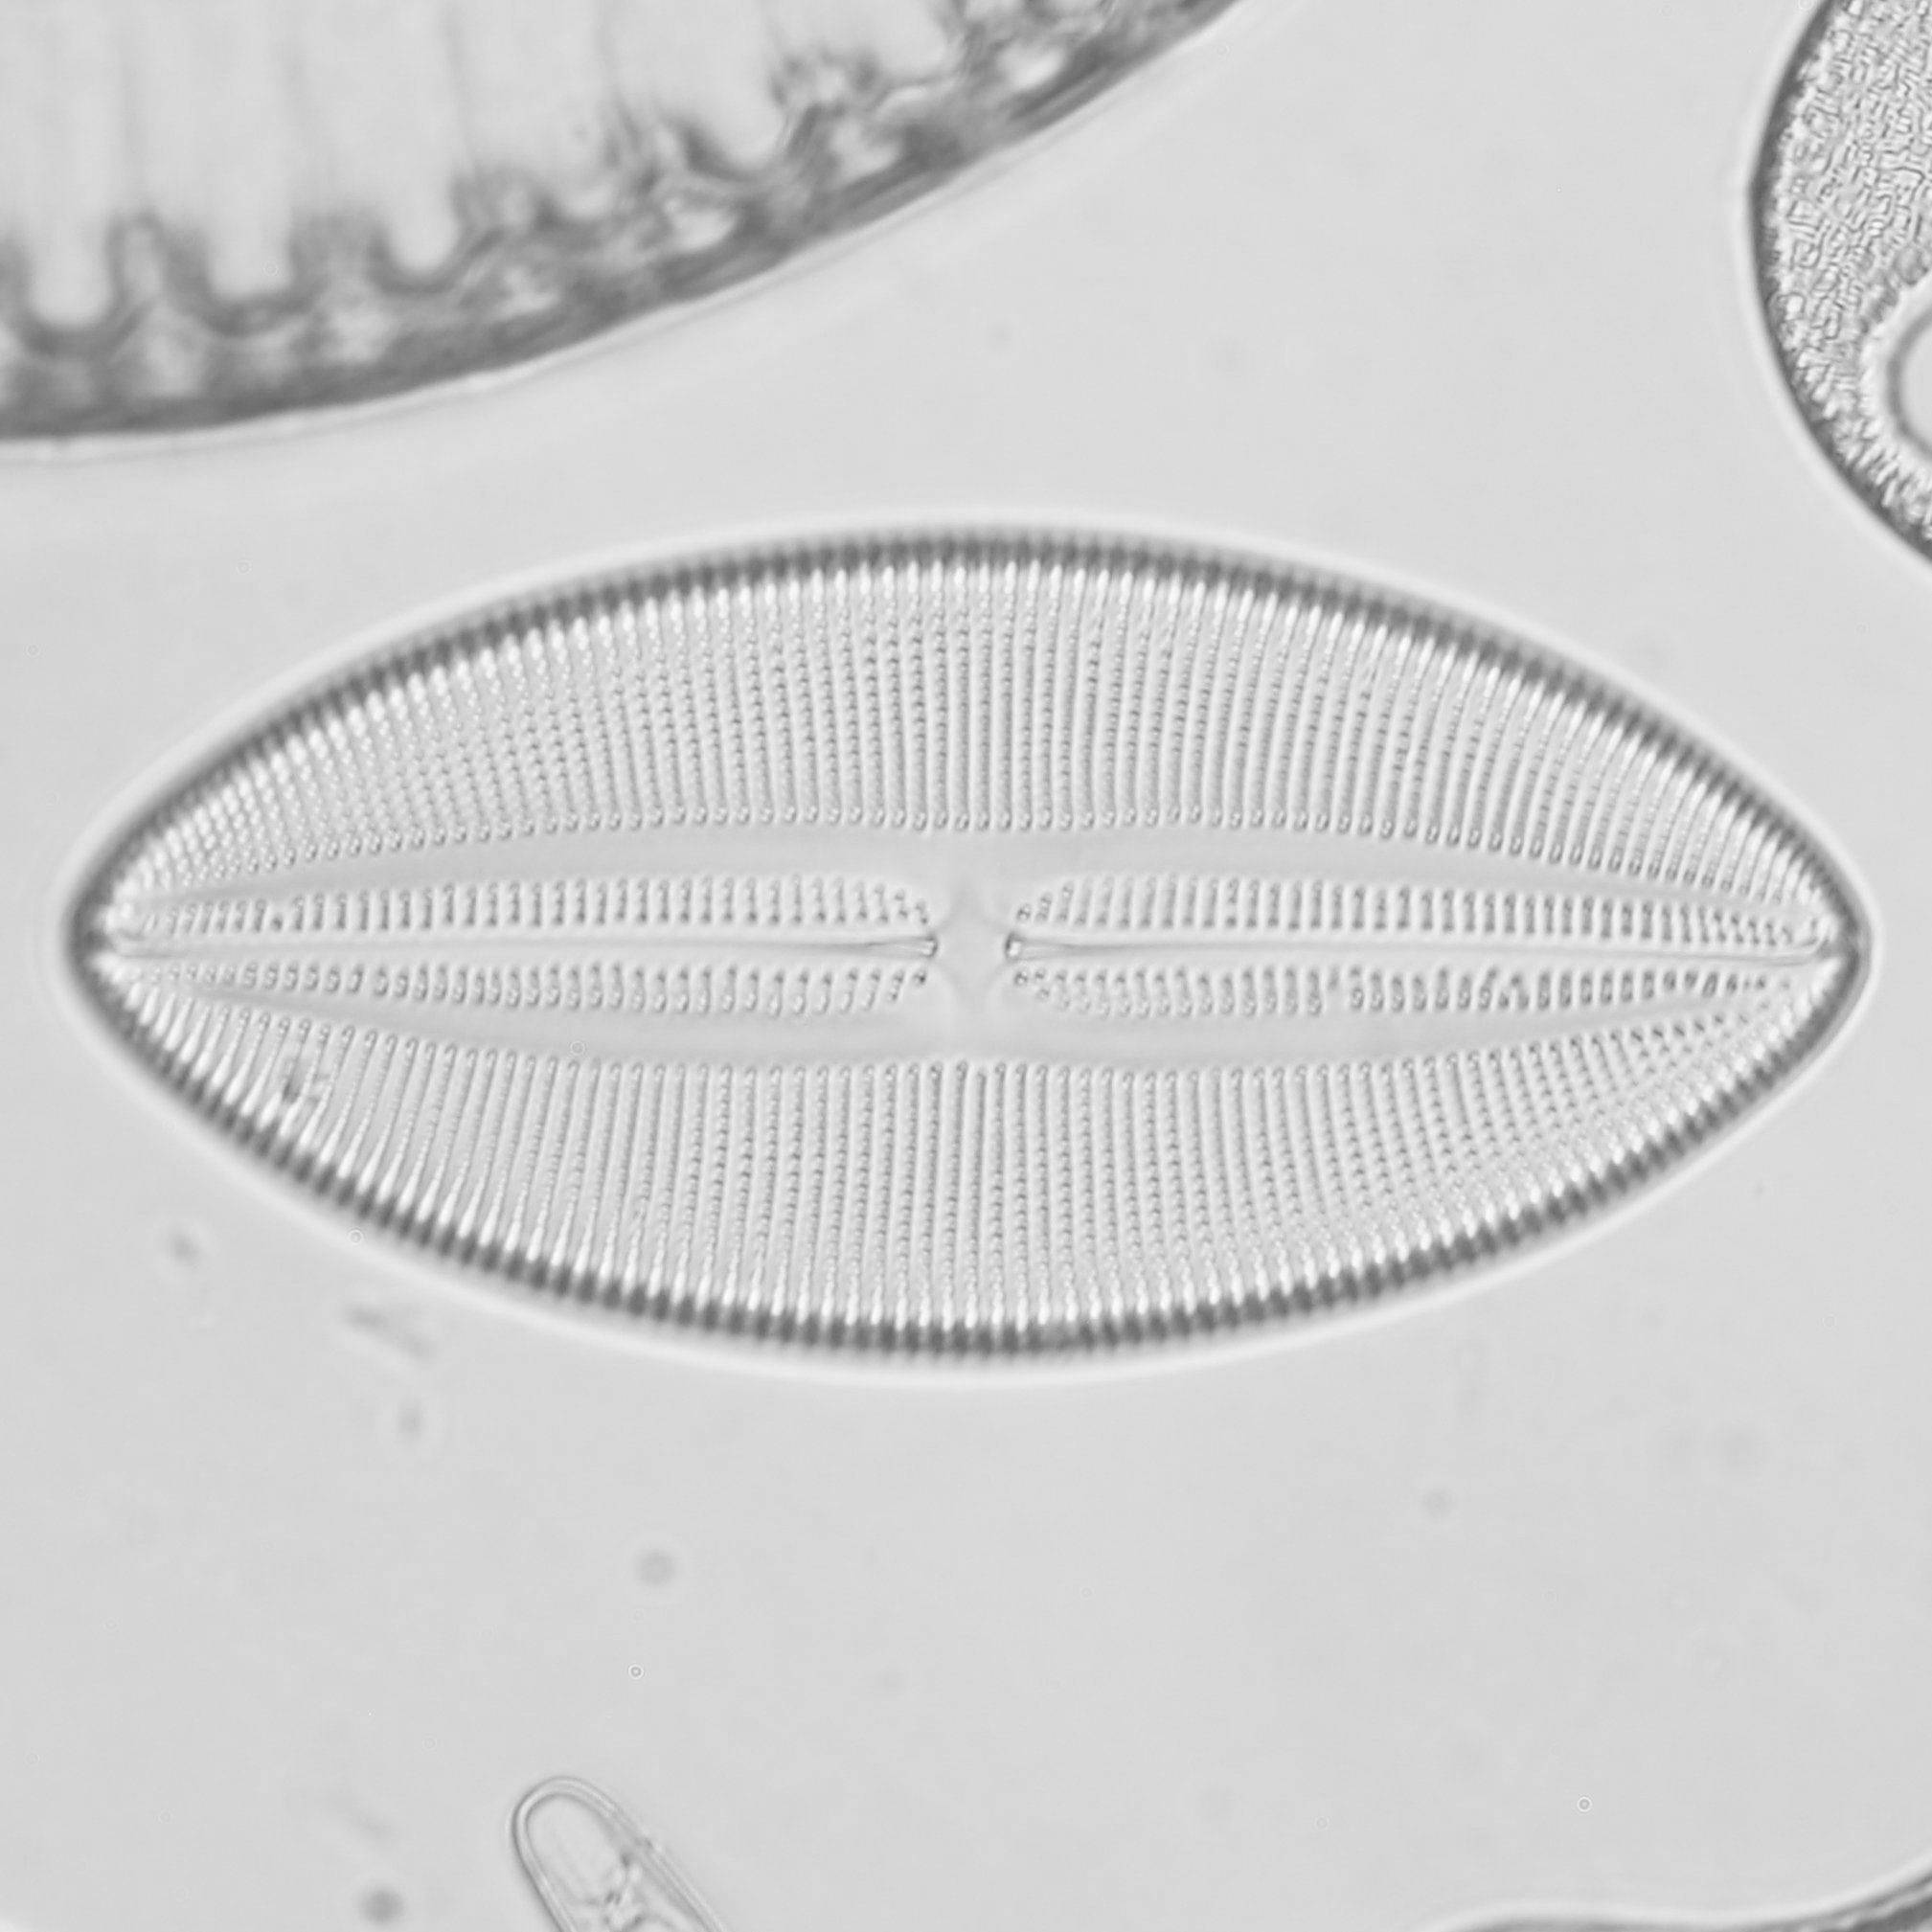
\includegraphics[width=.32\columnwidth]{Exp_2_Microphotography/Figures/10_Diatome_brightfield_03_cropped_32}} \hspace{0.1mm}
\subfloat[Normalized 0\%\label{diatnor}]{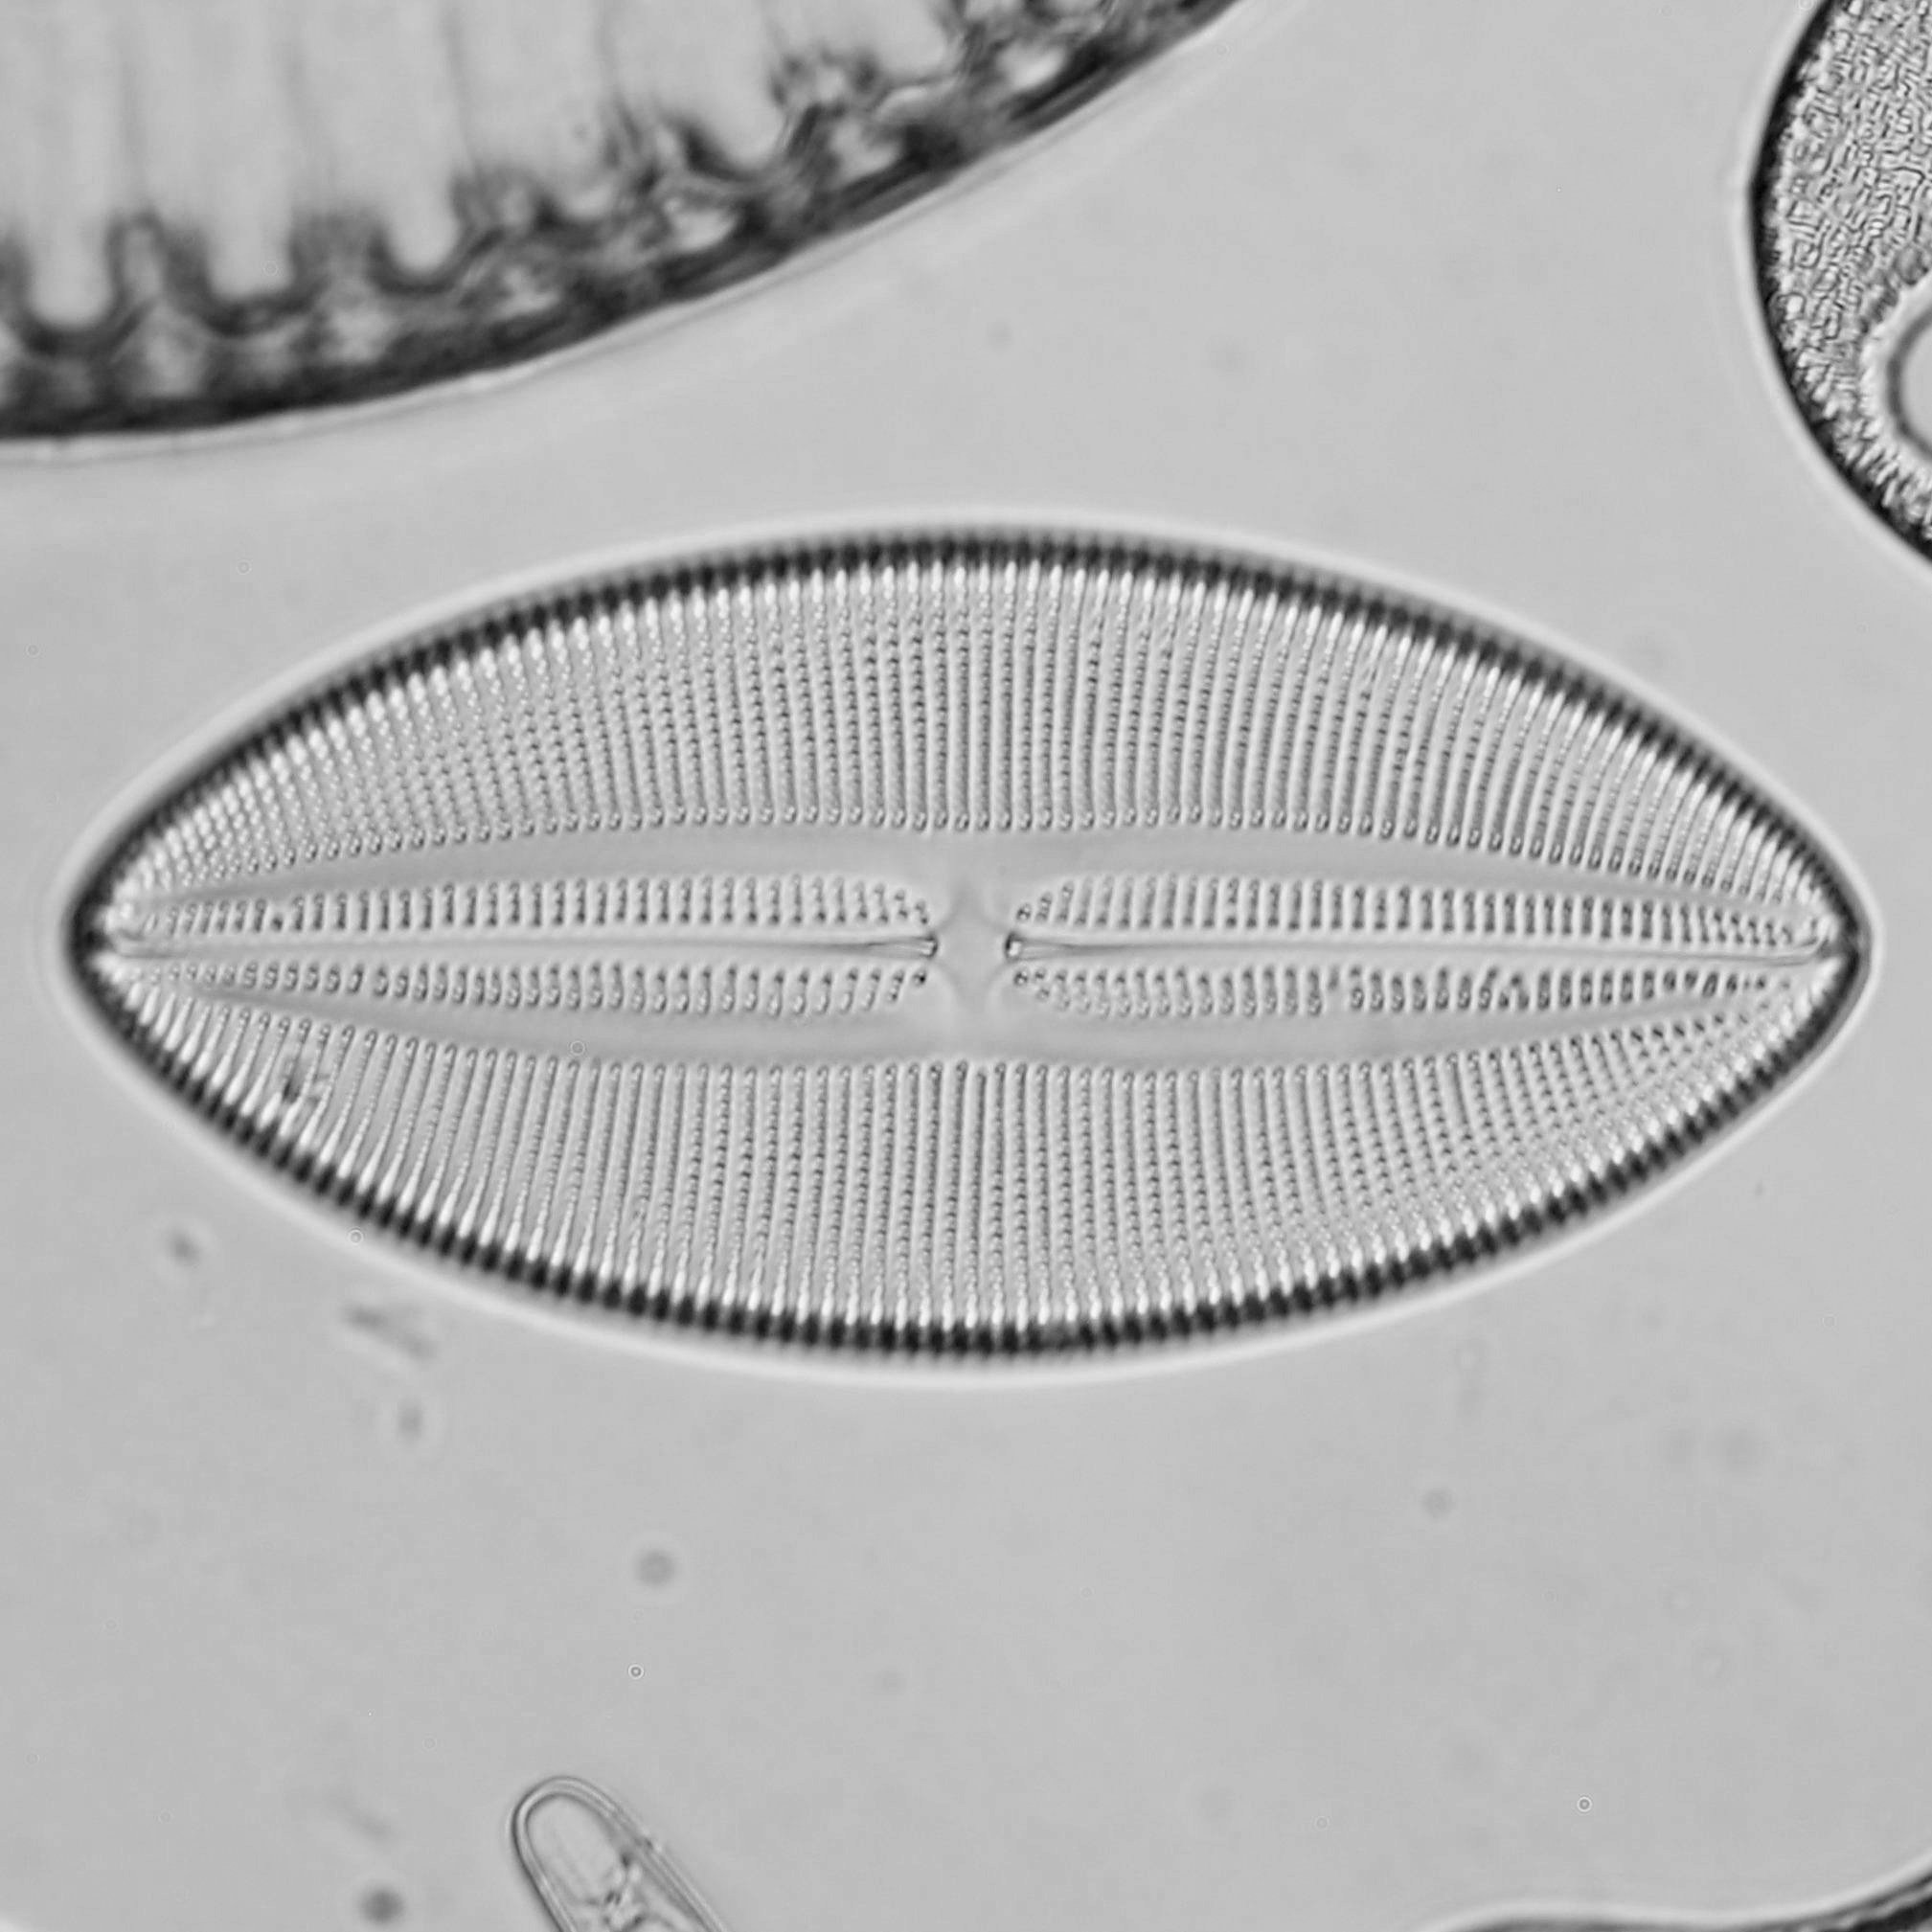
\includegraphics[width=.32\columnwidth]{Exp_2_Microphotography/Figures/10_Diatome_brightfield_03_cropped_32_000norm}} \hspace{0.1mm}
\subfloat[Manual Adjustment\label{diatman}]{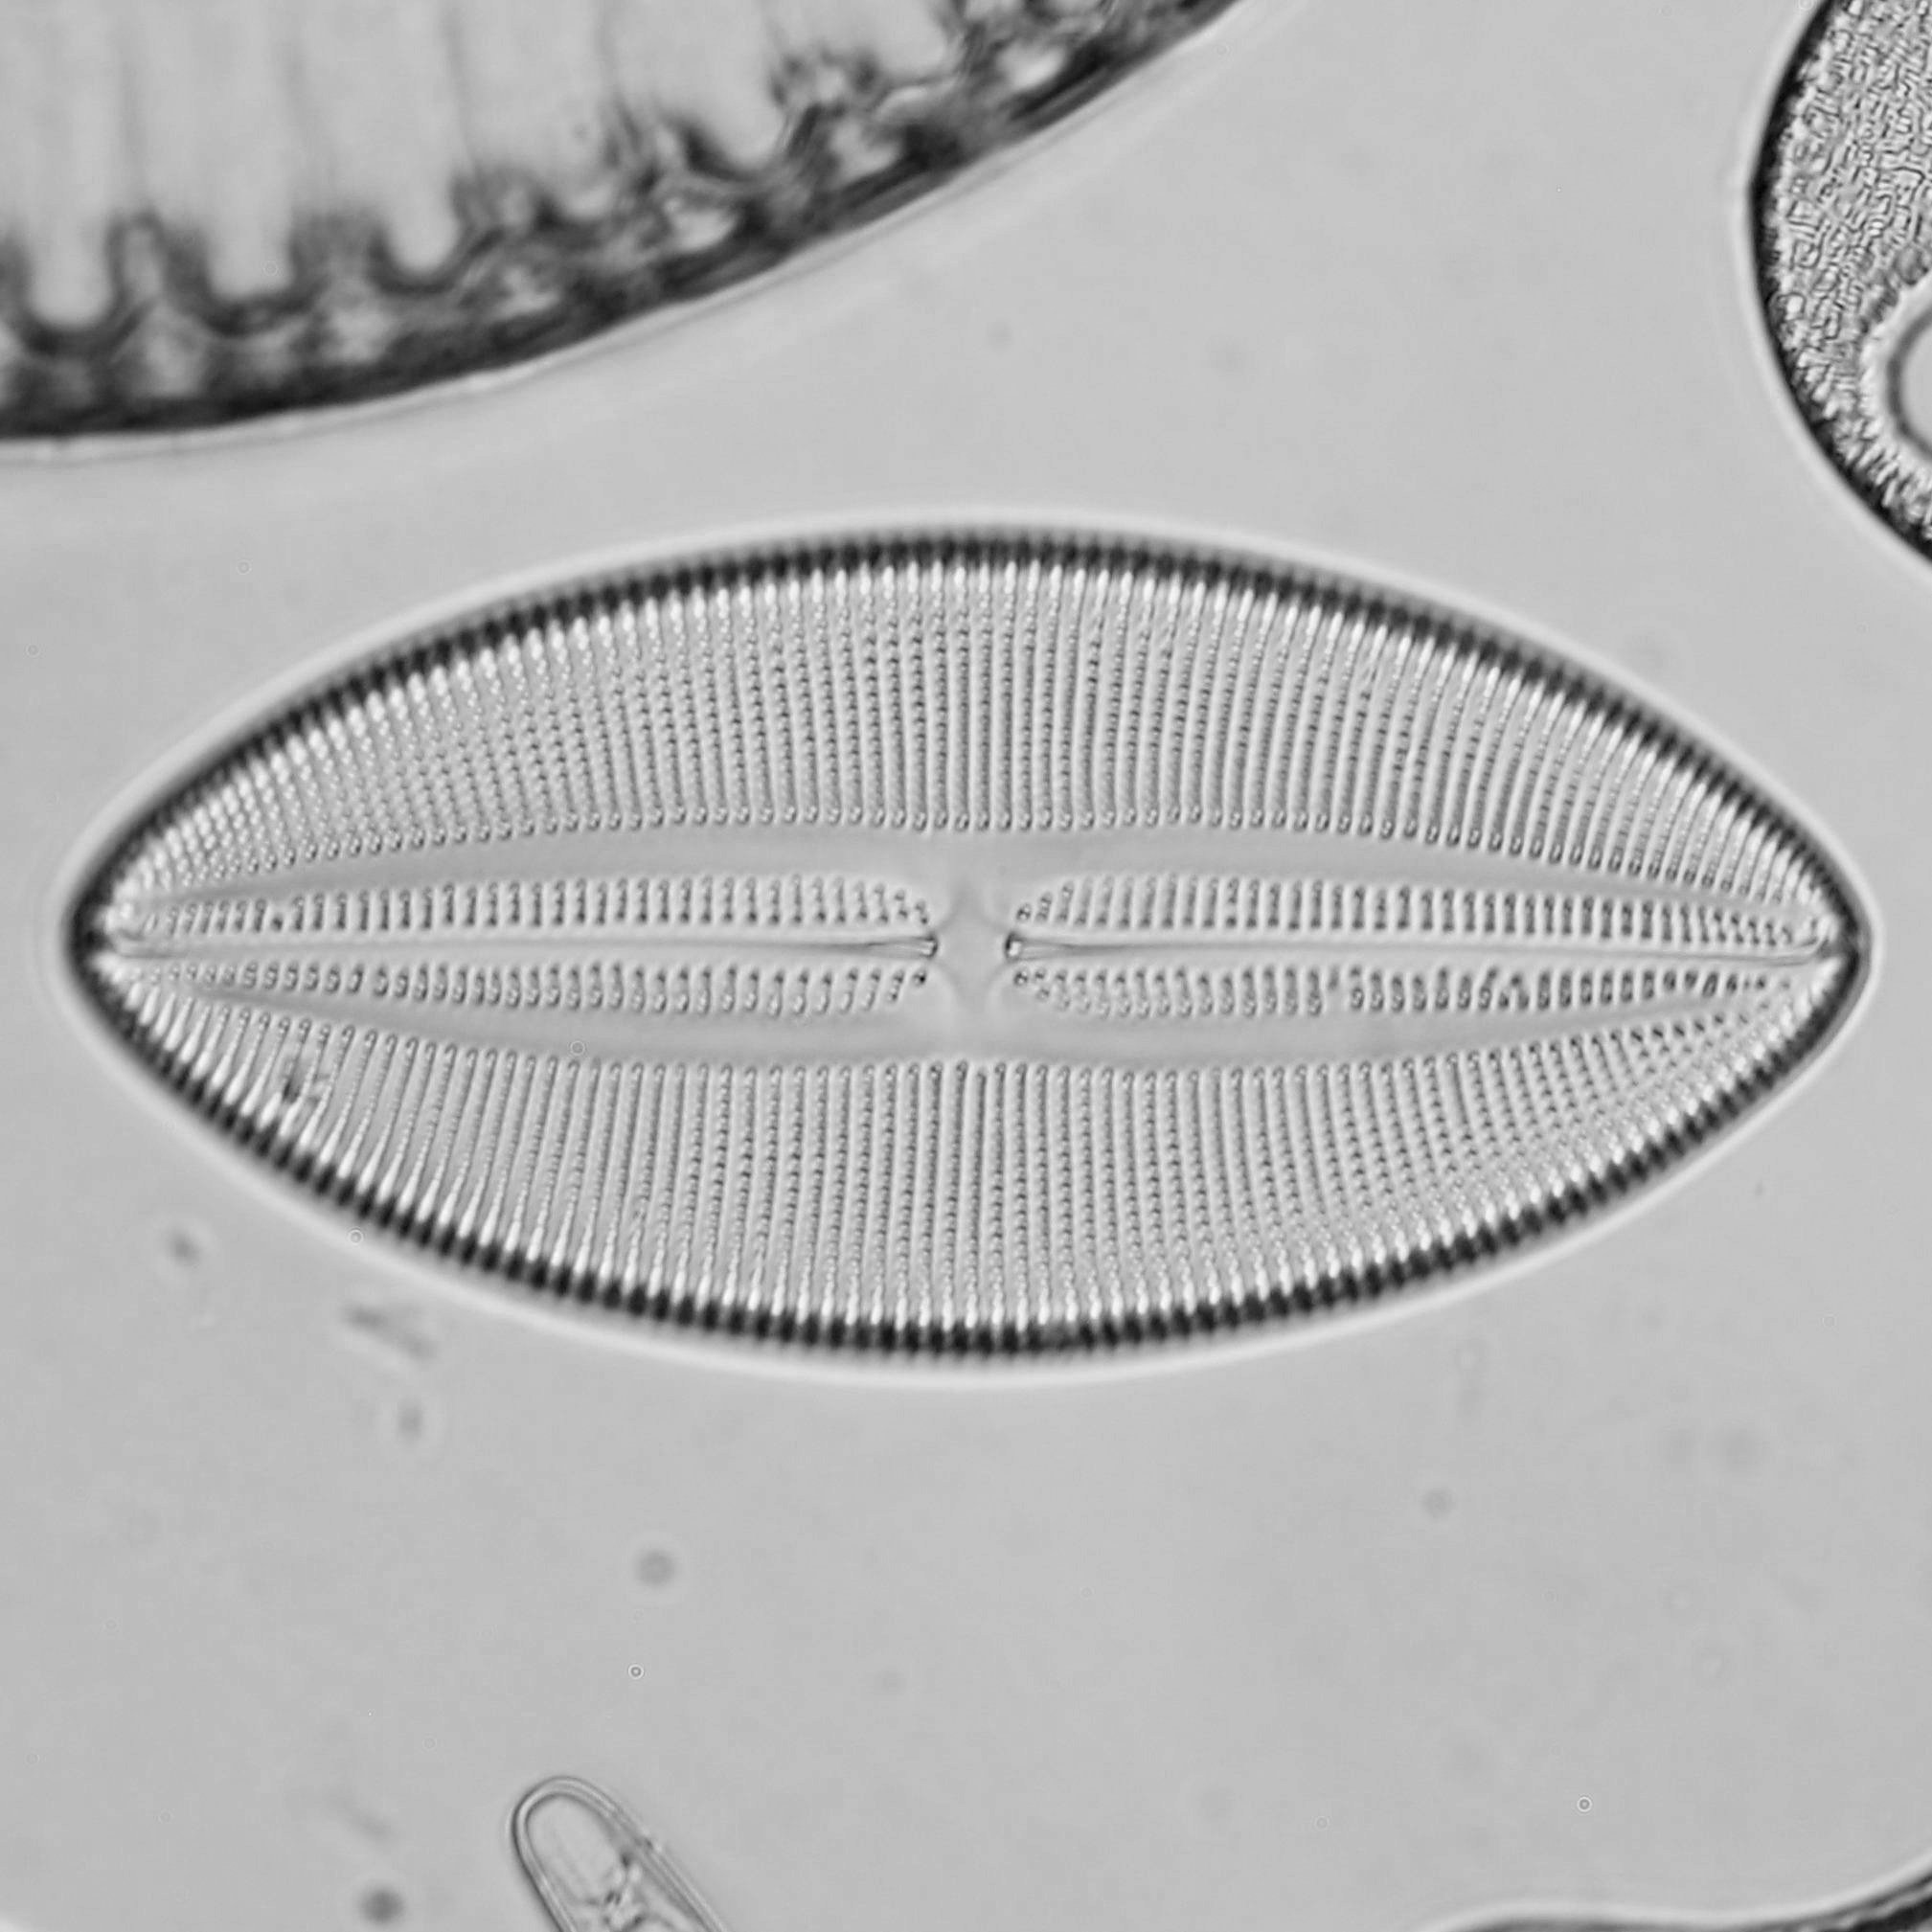
\includegraphics[width=.32\columnwidth]{Exp_2_Microphotography/Figures/10_Diatome_brightfield_03_cropped_32_000norm}}\vspace{-0.7em} 
\captionsetup[subfigure]{position=bottom}
\subfloat{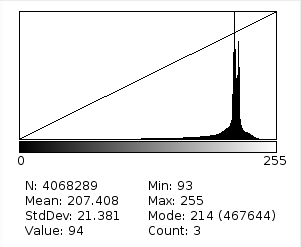
\includegraphics[width=.32\columnwidth]{Exp_2_Microphotography/Figures/10_DIatomeBrightfield_NoStretch_line0-255}} \hspace{0.1mm}
\subfloat{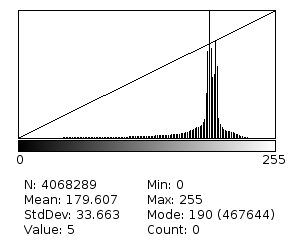
\includegraphics[width=.32\columnwidth]{Exp_2_Microphotography/Figures/10_DIatomeBrightfield_Stretch_line0-255}} \hspace{0.1mm}
\subfloat{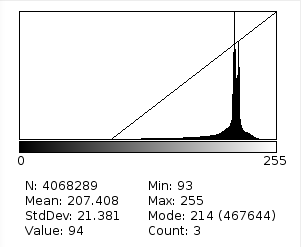
\includegraphics[width=.32\columnwidth]{Exp_2_Microphotography/Figures/10_DIatomeBrightfield_NoStretch_line93-255}}
\caption{Example of contast enhancement by normalization. 
%\textbf{A} is not normalized, \textbf{B} is normalized with 0\% saturation, \textbf{C} is adjusted manually. 
Diagonals in the histograms are added manually, no scale bar presented, images are for illustrative purposes only.}
\label{fig:normcompare}
\end{figure}

Two findings of using this procedure: One, this procedure does not significantly improve the quality of some images, e.g darkfield images, which has already good contrast. 
Nevertheless this method was done to such images anyway due to the workflow and the results are not at all detrimental for visualization and assesment. 
In other words, no significant differences could be observed between the normalized ones and the ones adjusted manually (compare Fig.~\ref{diatnor} and Fig.~\ref{diatman}). 

\begin{figure}[h!]
\centering
\captionsetup[subfigure]{position=top}
\subfloat[Not normalized\label{fluono}]{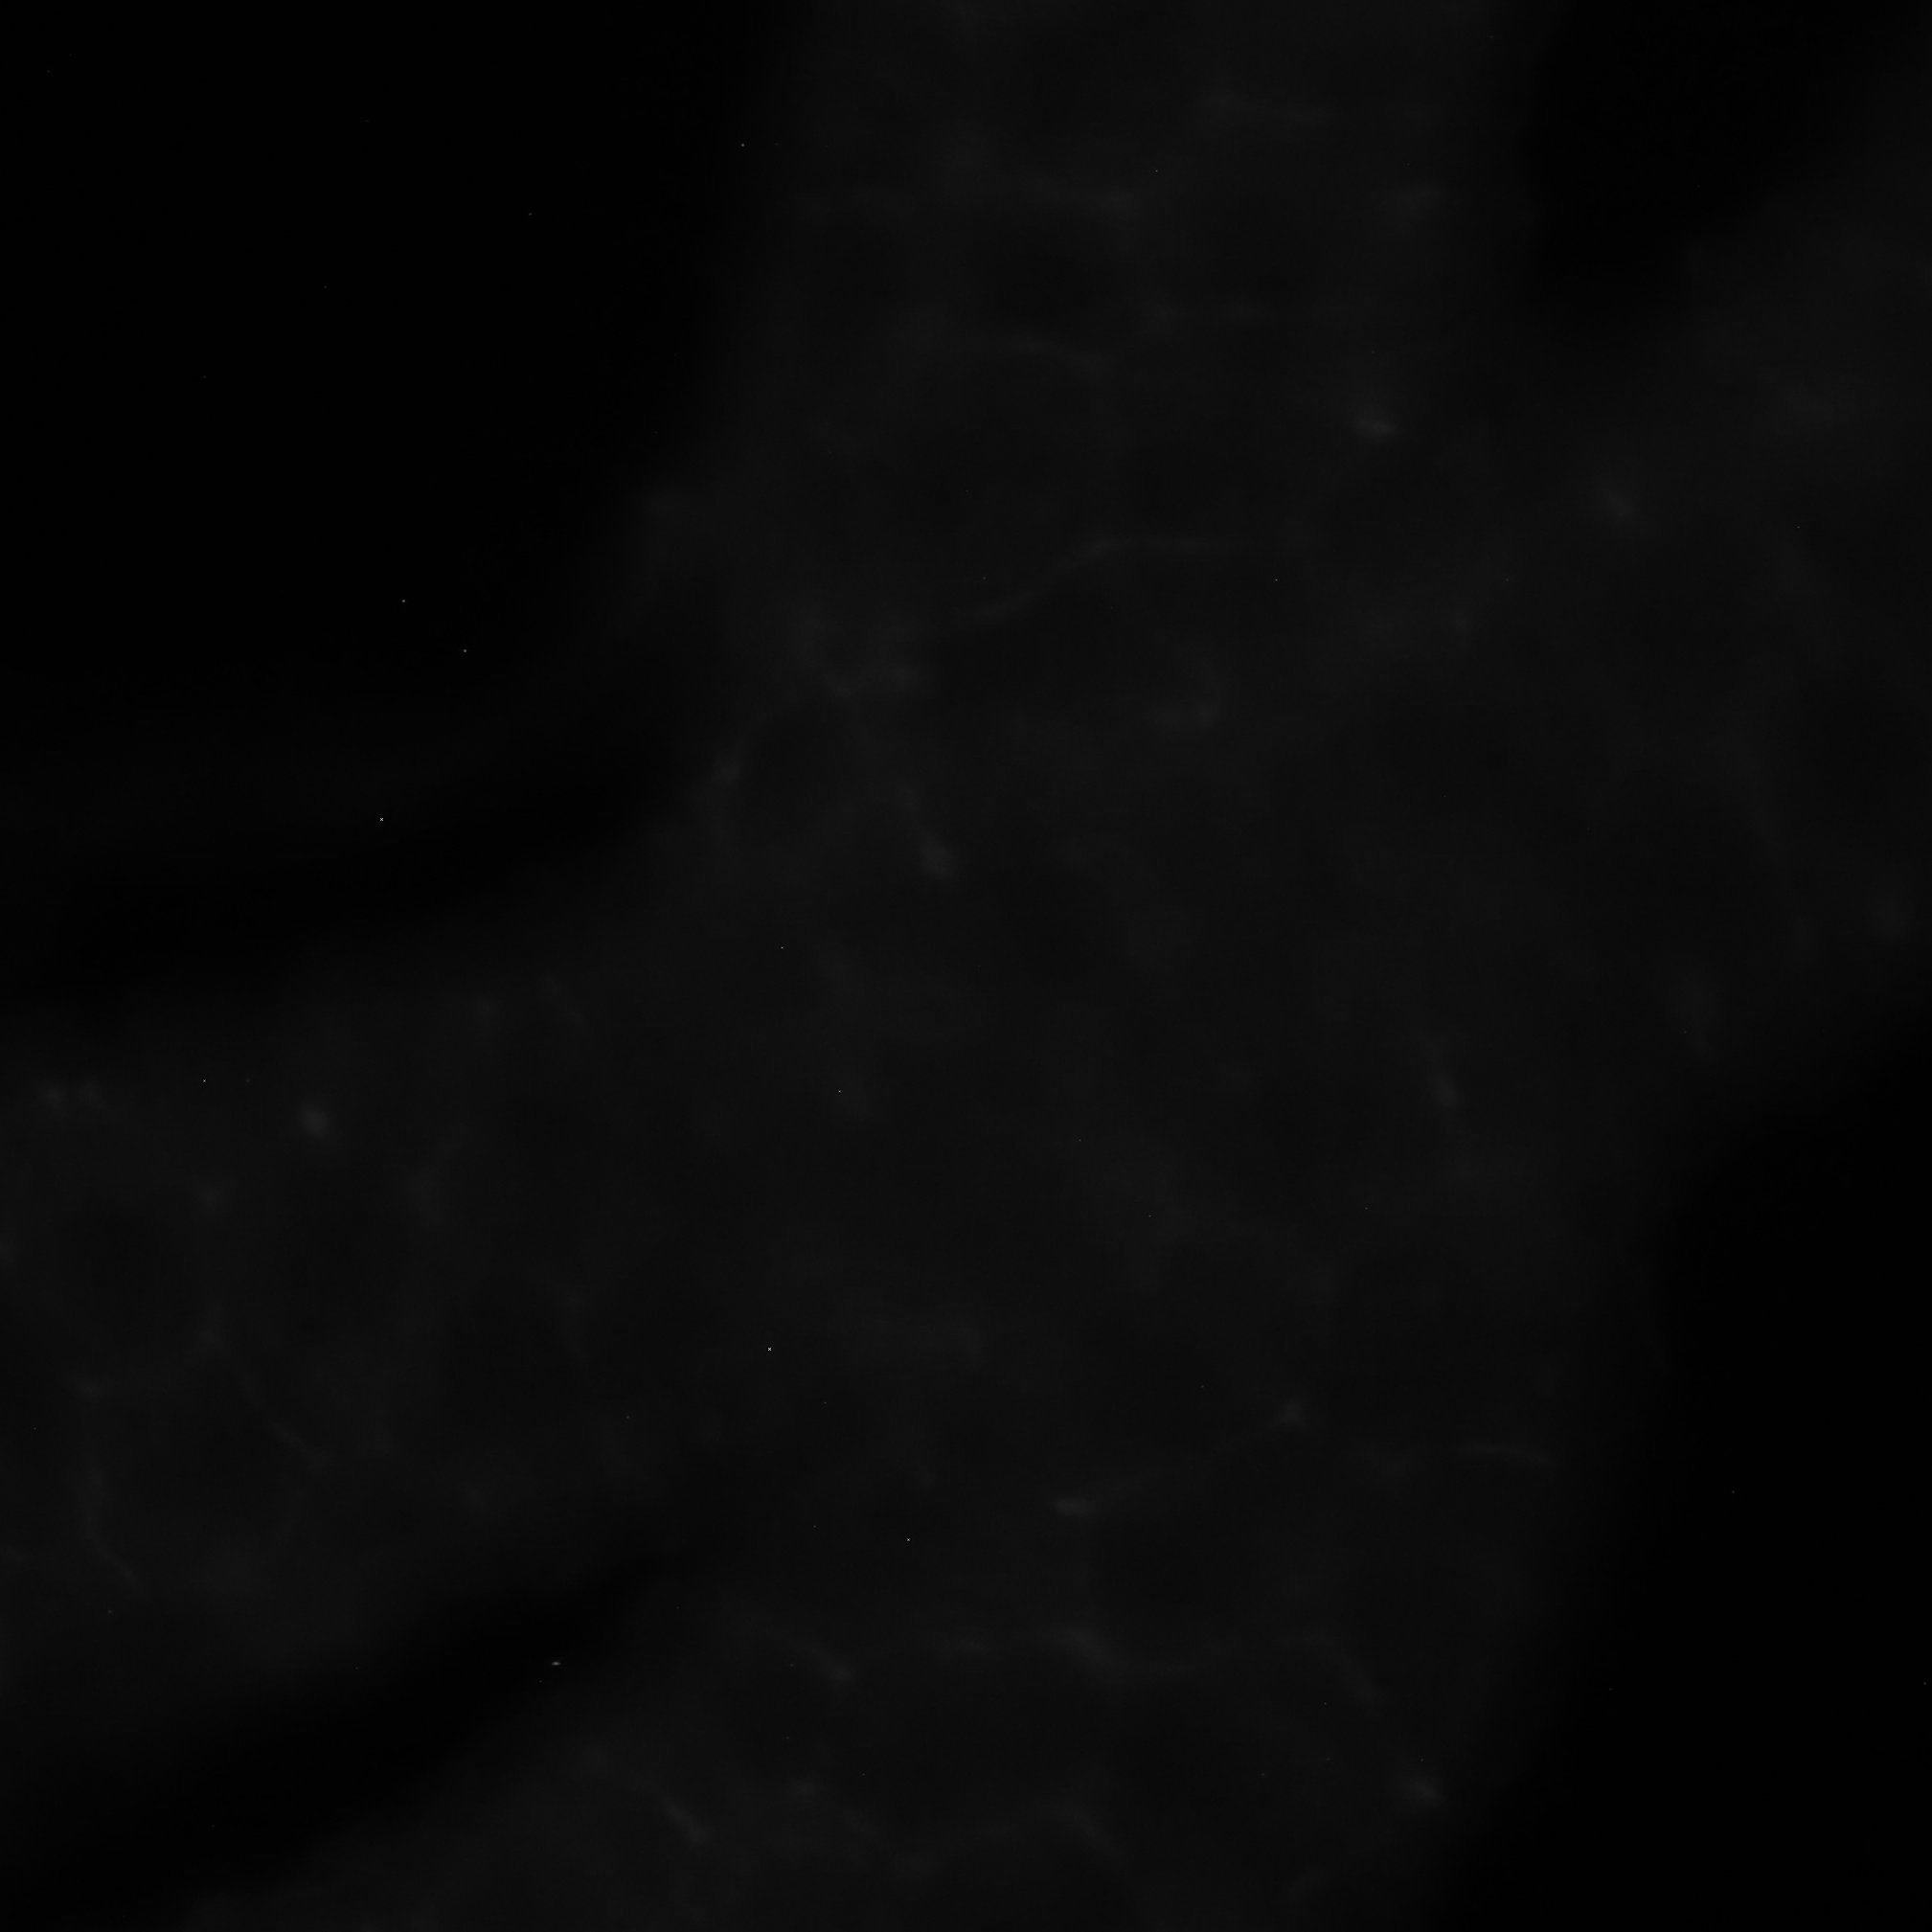
\includegraphics[width=.32\columnwidth]{Exp_2_Microphotography/Figures/redfluononorm_cropped_32}} \hspace{0.1mm}
\subfloat[Normalized 0\%\label{fluo0}]{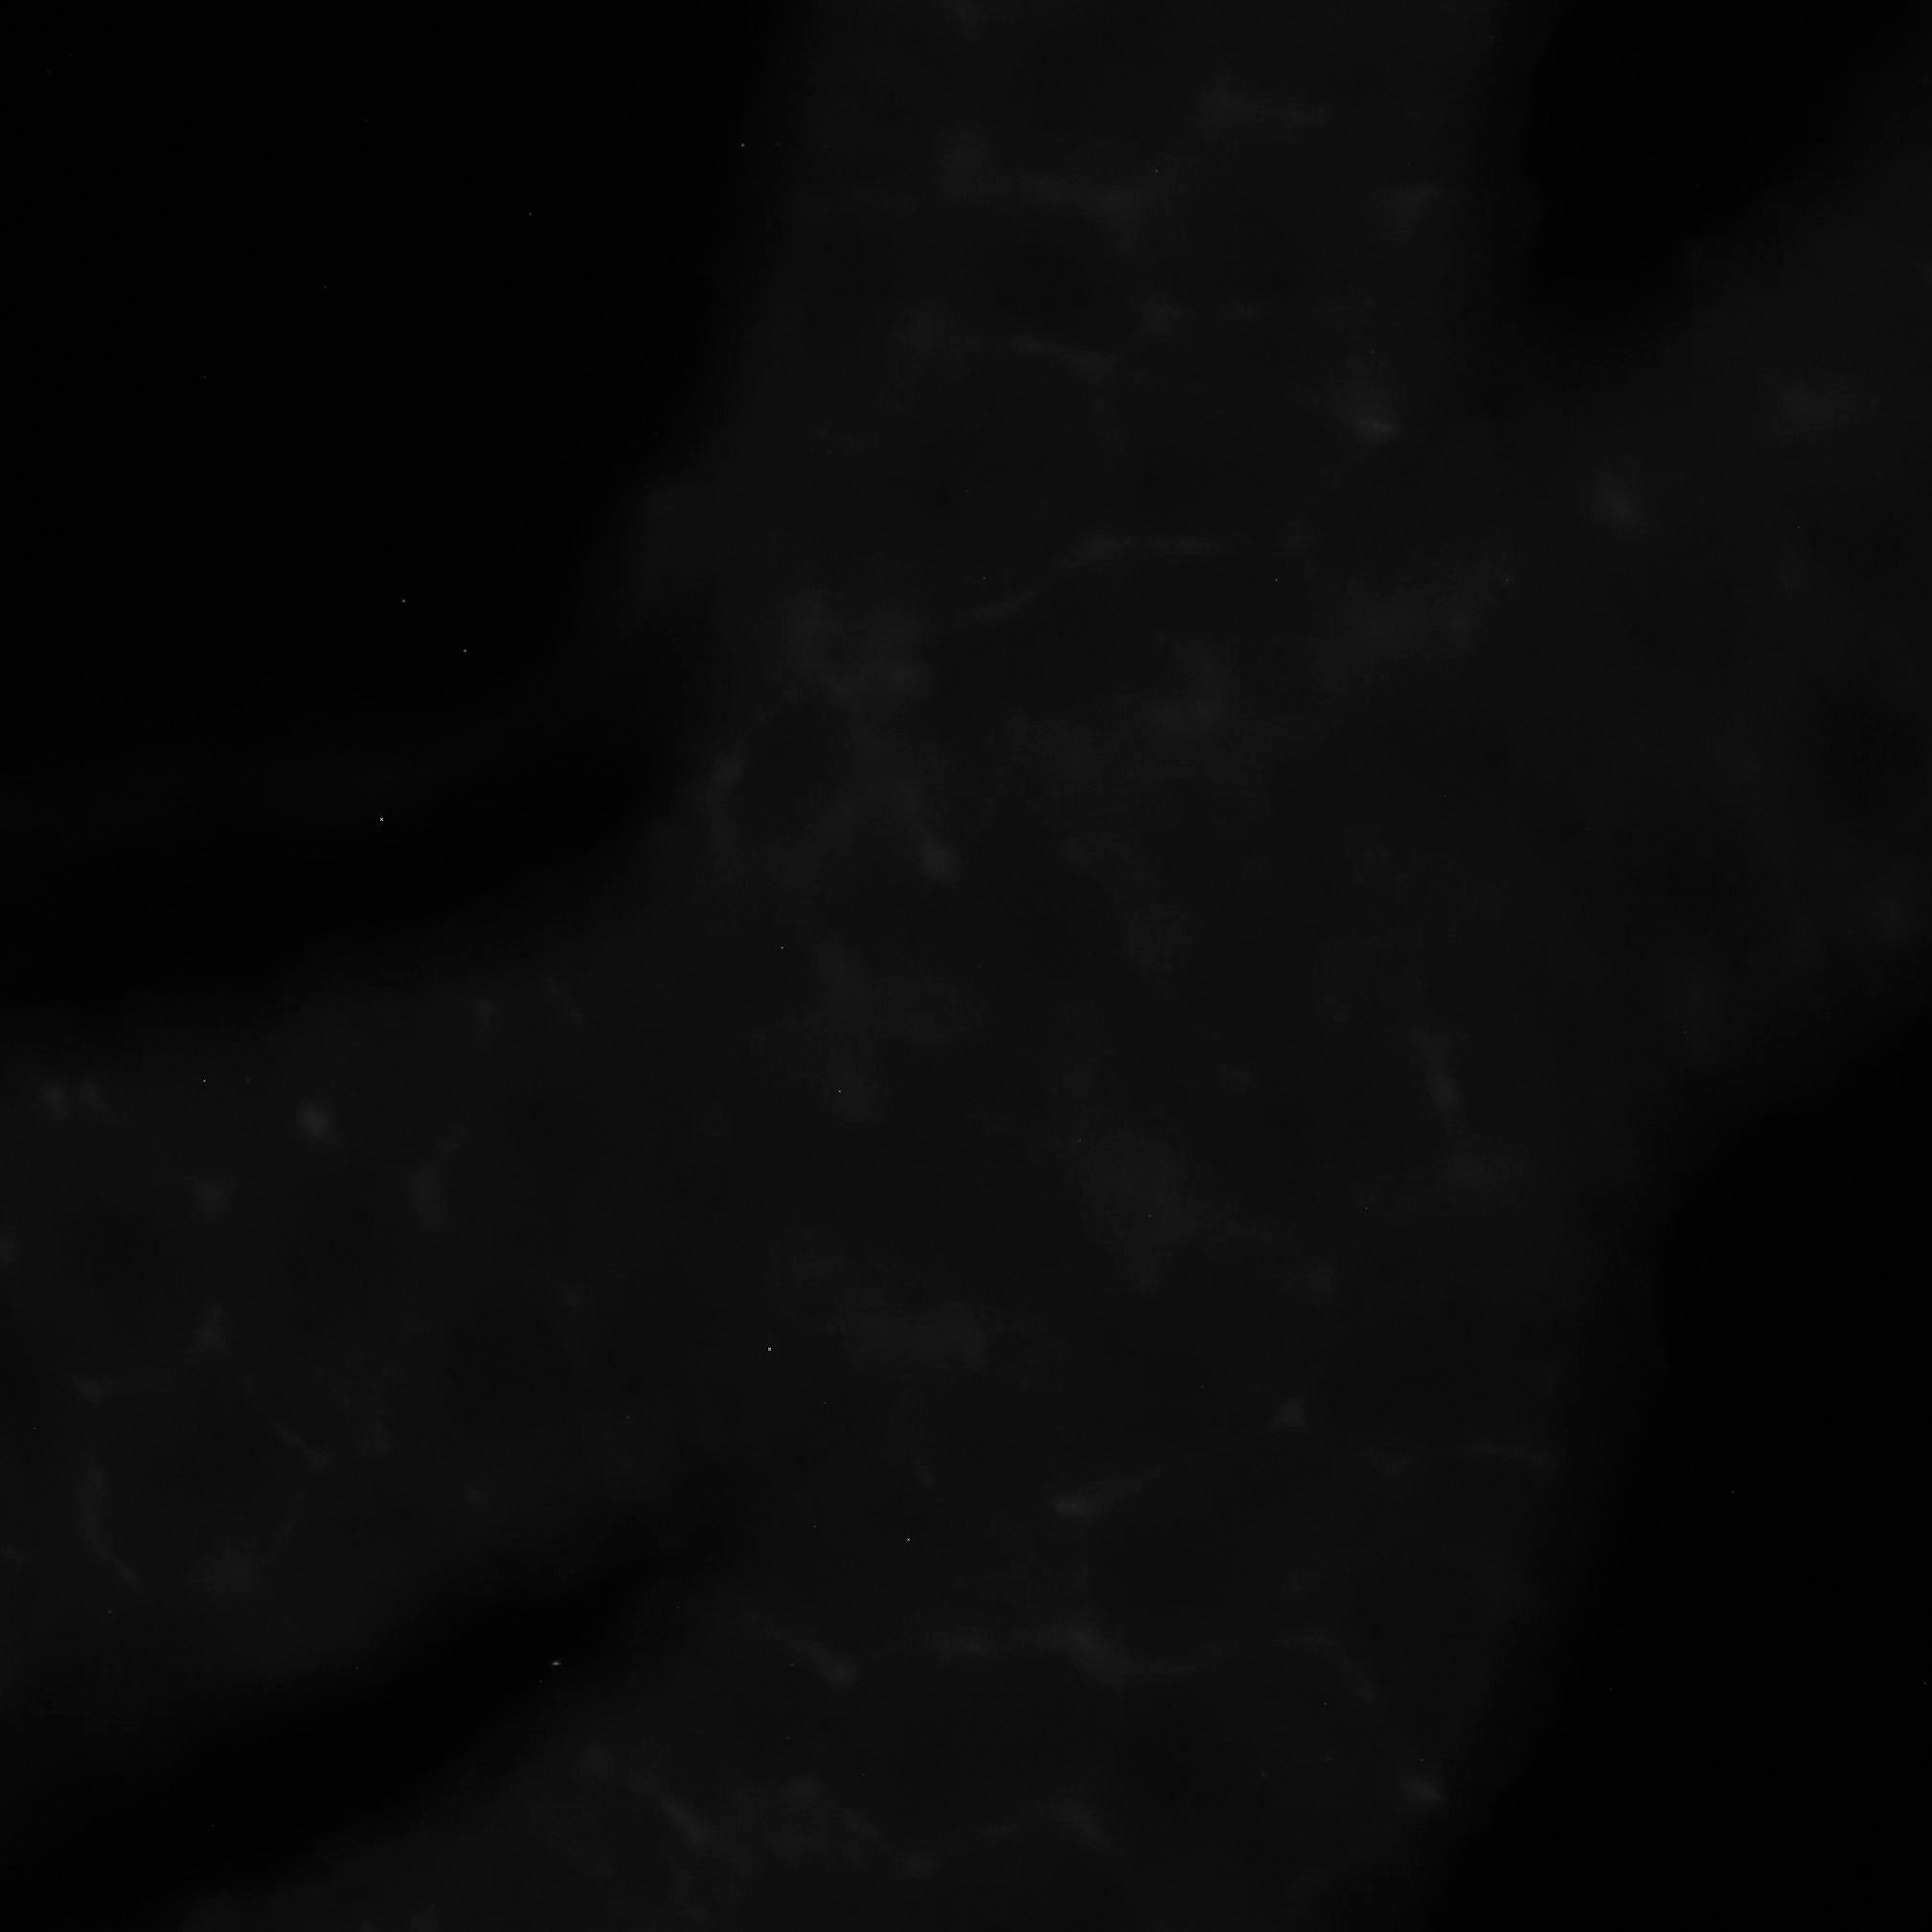
\includegraphics[width=.32\columnwidth]{Exp_2_Microphotography/Figures/redfluo0norm_cropped_32}} \hspace{0.1mm}
\subfloat[Normalized 0.01\%\label{fluo1}]{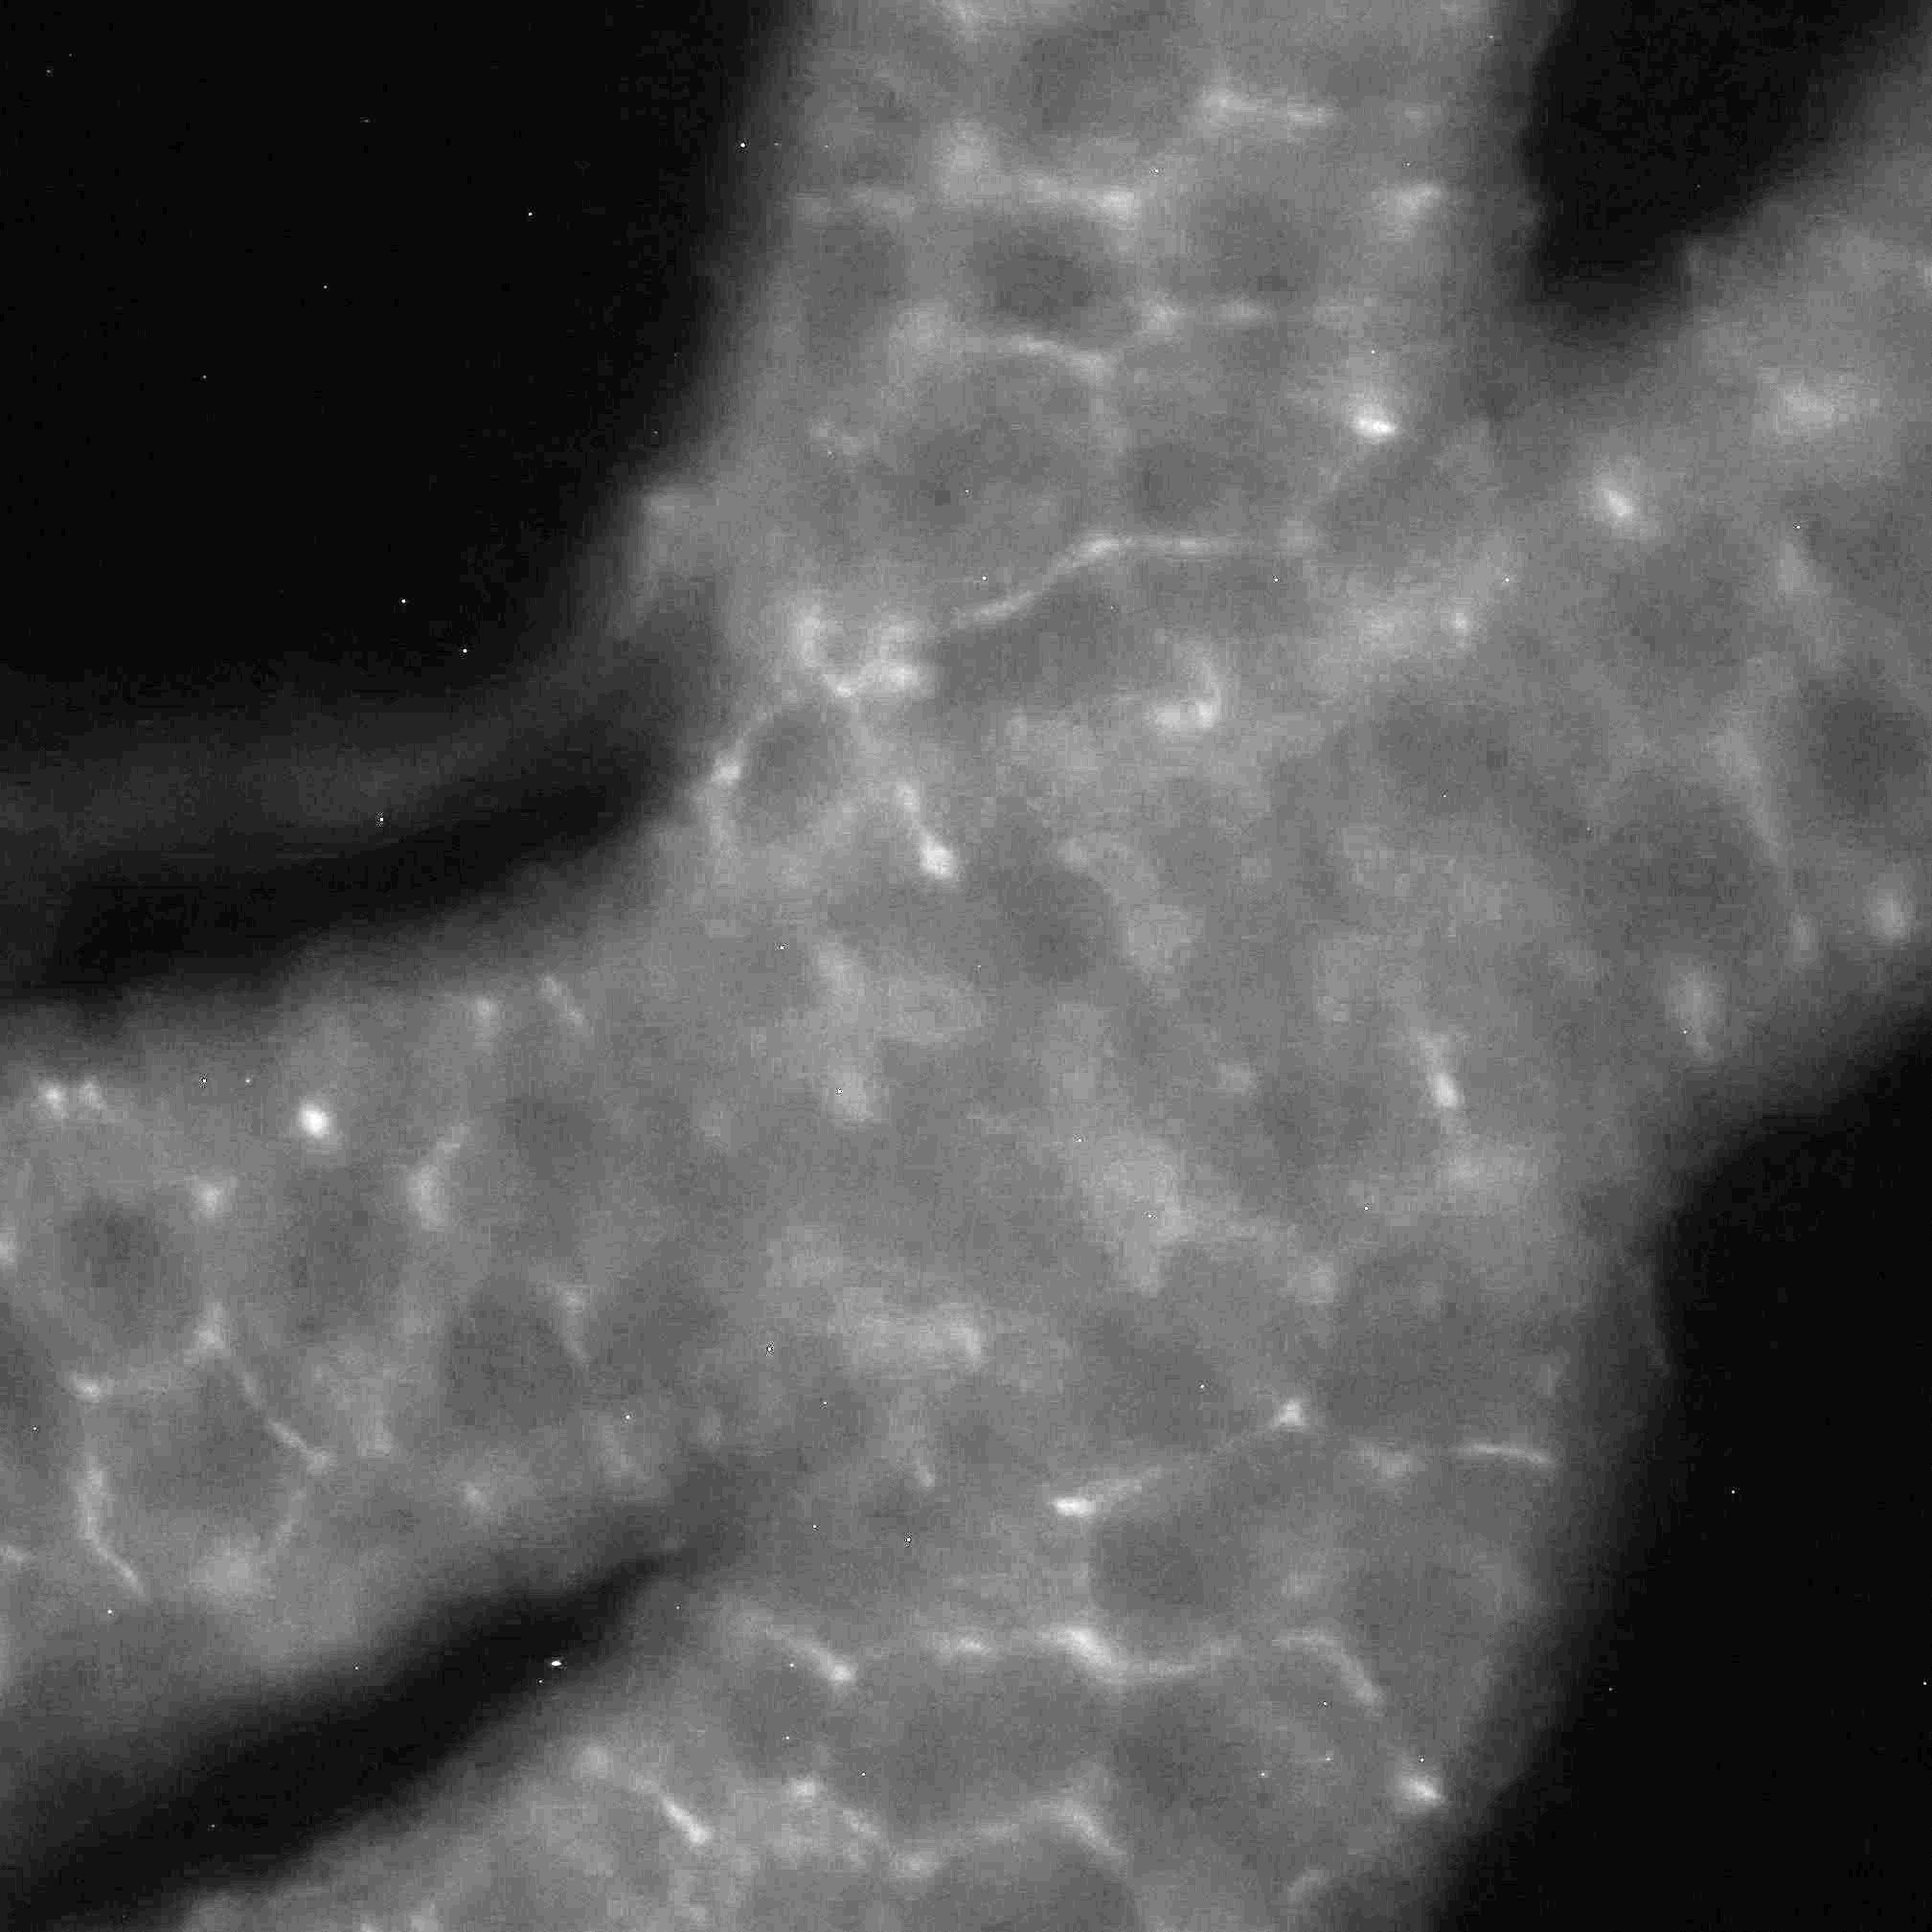
\includegraphics[width=.32\columnwidth]{Exp_2_Microphotography/Figures/redfluo001norm_cropped_32}}\vspace{-0.7em} 
\captionsetup[subfigure]{position=bottom}
\subfloat{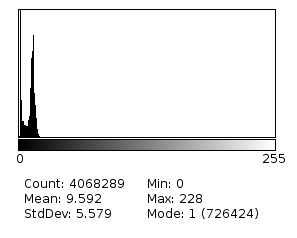
\includegraphics[width=.32\columnwidth]{Exp_2_Microphotography/Figures/redfluononorm}} \hspace{0.1mm}
\subfloat{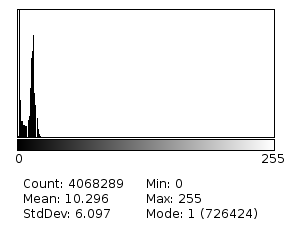
\includegraphics[width=.32\columnwidth]{Exp_2_Microphotography/Figures/redfluo0norm}} \hspace{0.1mm}
\subfloat{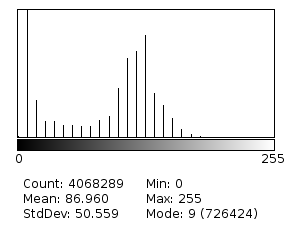
\includegraphics[width=.32\columnwidth]{Exp_2_Microphotography/Figures/redfluo001norm}}
\caption{Example of removing outlier values by normalization. 
%\textbf{A} is not normalized, \textbf{B} is normalized with 0\% saturation, \textbf{C} is normalized with 0.01 \% saturation. 
No scale bar presented, images are for illustrative purposes only.}
\label{fig:normprocedure}
\end{figure}

Two, this procedure were successful in enhancing the contrast for almost all other images except for some. 
Closer investigation of the histogram and pixel values of these images in detail (e.g blowfly fluorescence) found that there are some outliers at high pixel values. 
This is demonstrated by saturating (during normalization) at really low percentage (0.01\%) removes the outliers and enhanced the contrast significantly. 
As can be seen in Fig.~\ref{fig:normprocedure}. 
The grey-scaled but unnormalized image (Fig.~\ref{fluono}) of blowfly fluorescence is very dark and contrast enhancement is necessary. 
Applying the procedure without saturation (Fig.~\ref{fluo0}) does not improve the contrast at all. 
Just by adjusting the saturation to 0.01\% (Fig.~\ref{fluo1}) the contrast is improved dramatically. 
For consistency reasons, all images acquired from the same technique are treated the same, although this may not be strictly necessary. 
However since the saturation amount is practically negligible, this should not hinder the purpose of visualization of the images in this report. 

%------------------------------
\subsection{Diatoms}

\begin{figure}[h]
\centering
\captionsetup[subfigure]{position=top}
\subfloat[Brightfield\label{dbright}]{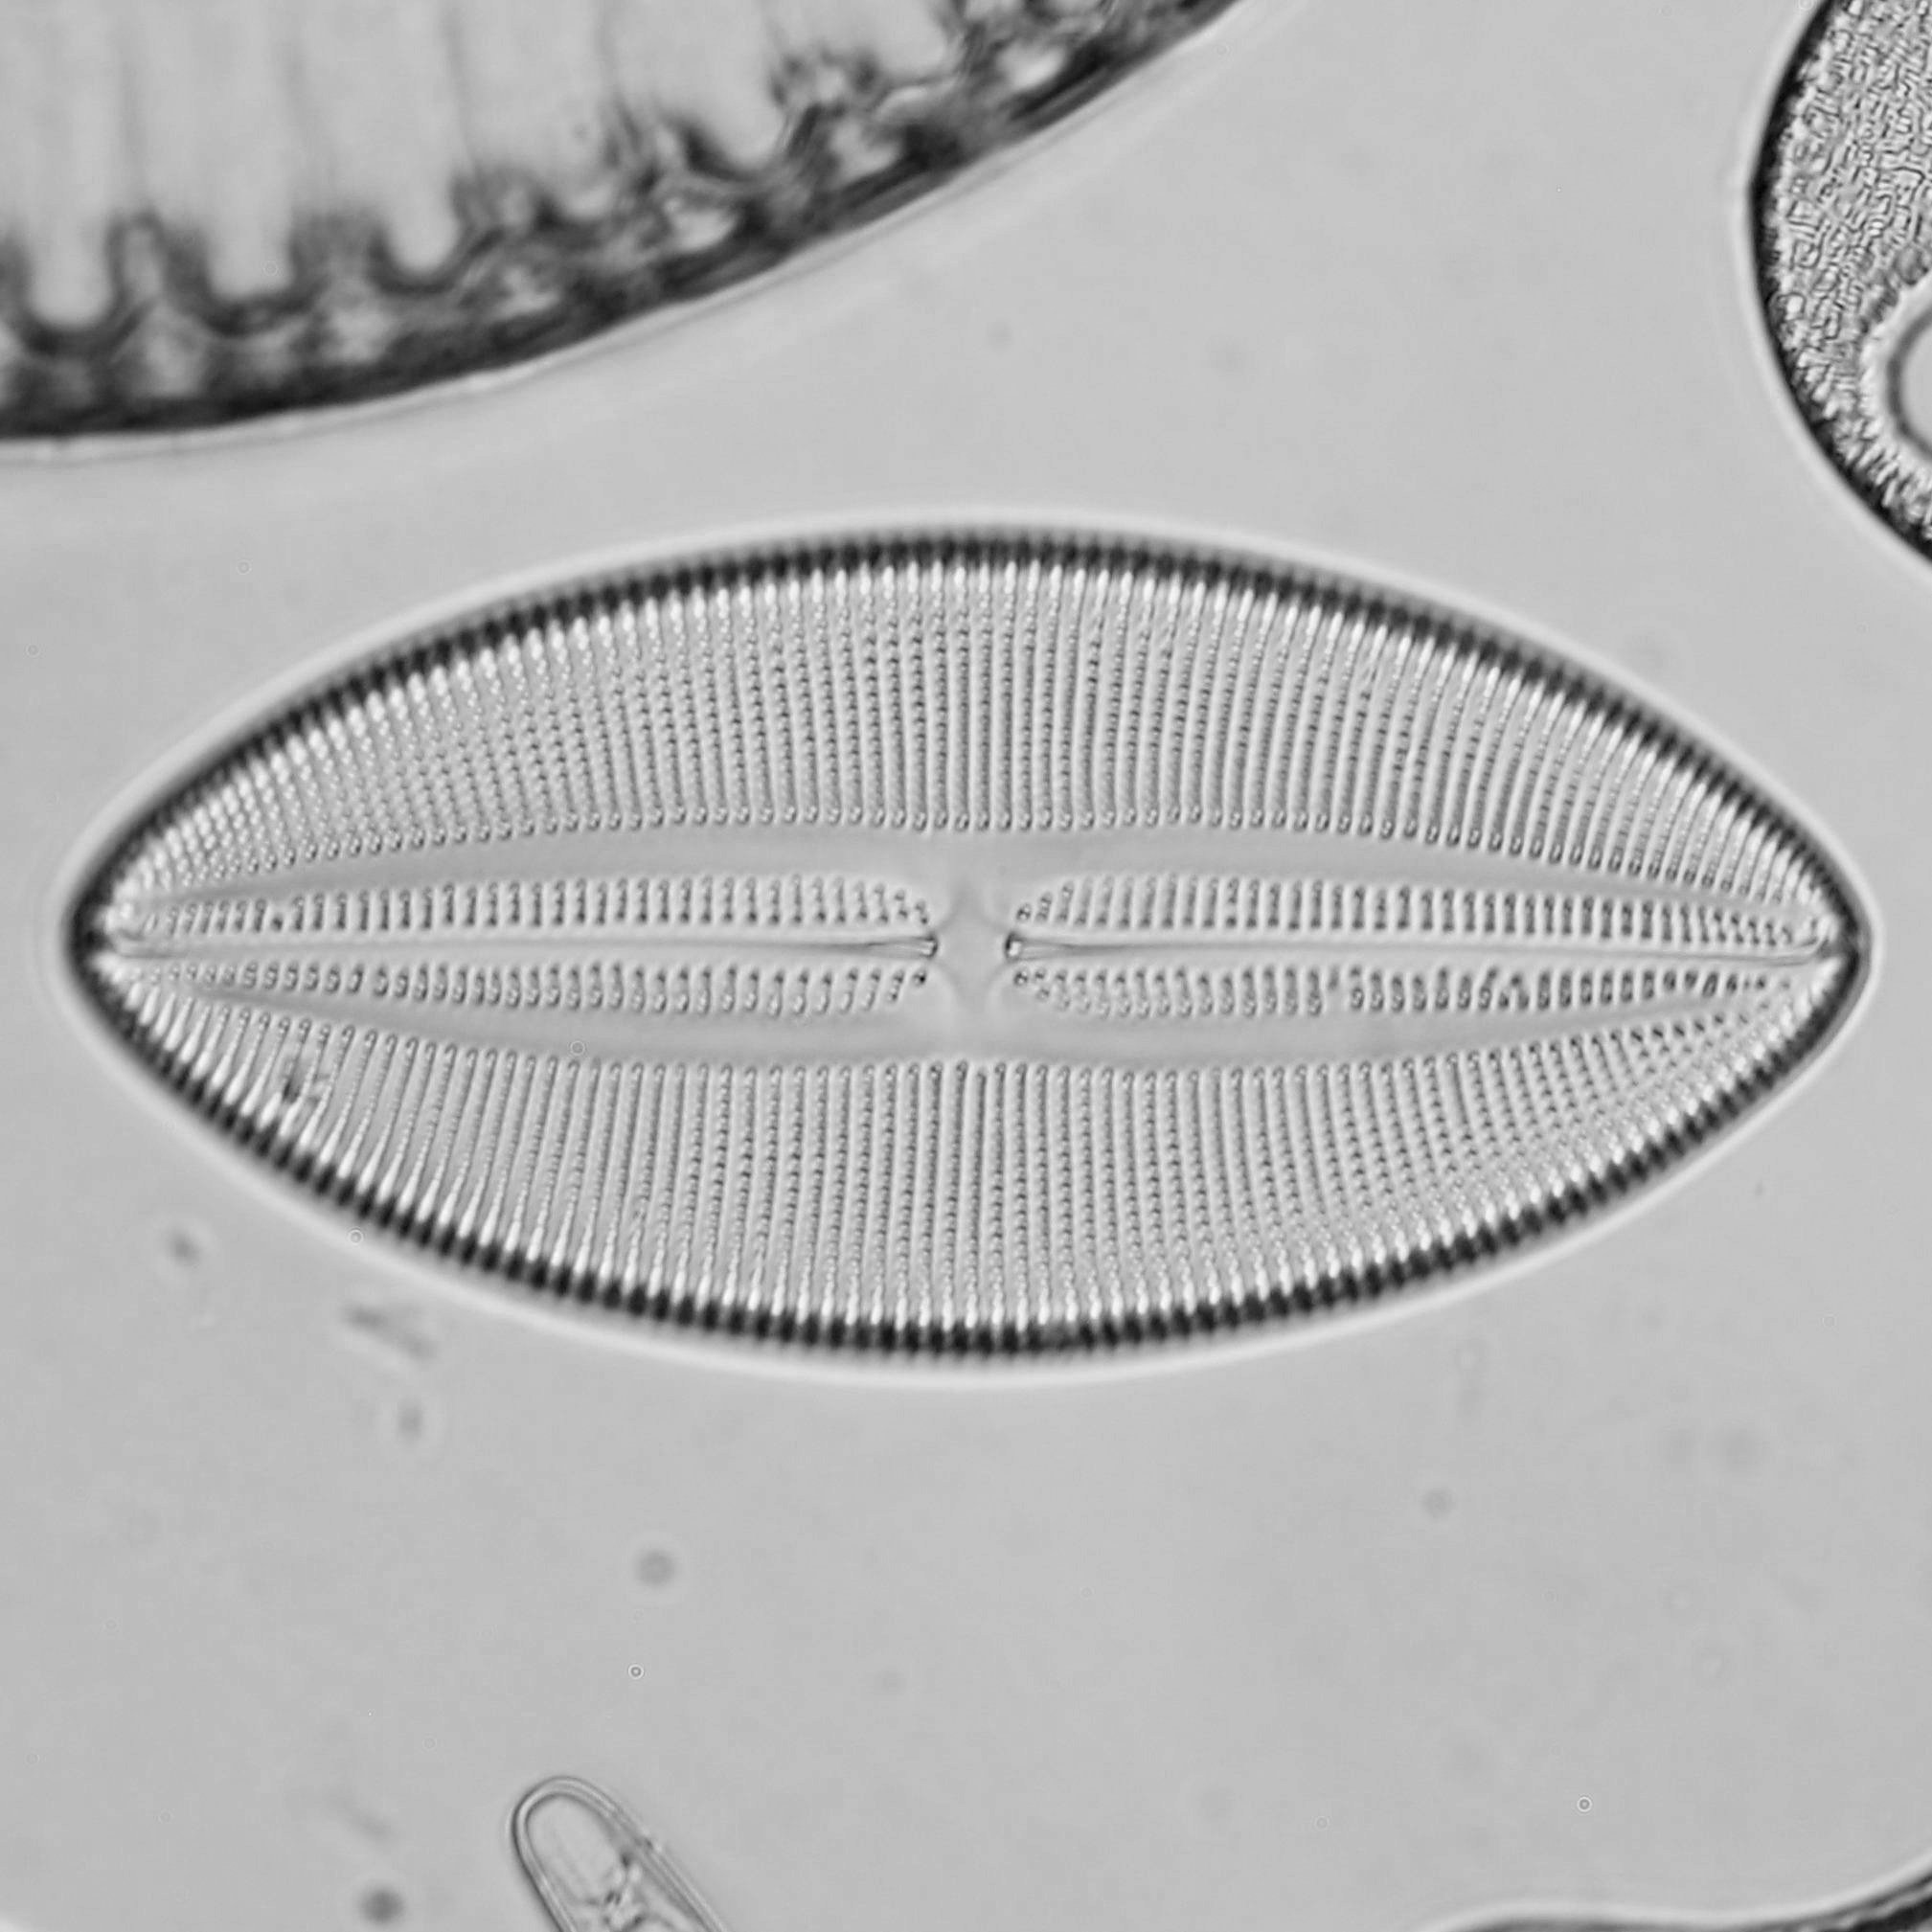
\includegraphics[width=.32\columnwidth]{Exp_2_Microphotography/Figures/10_Diatome_brightfield_03_cropped_32_000norm}} \hspace{0.1mm}
\subfloat[Darkfield\label{ddark}]{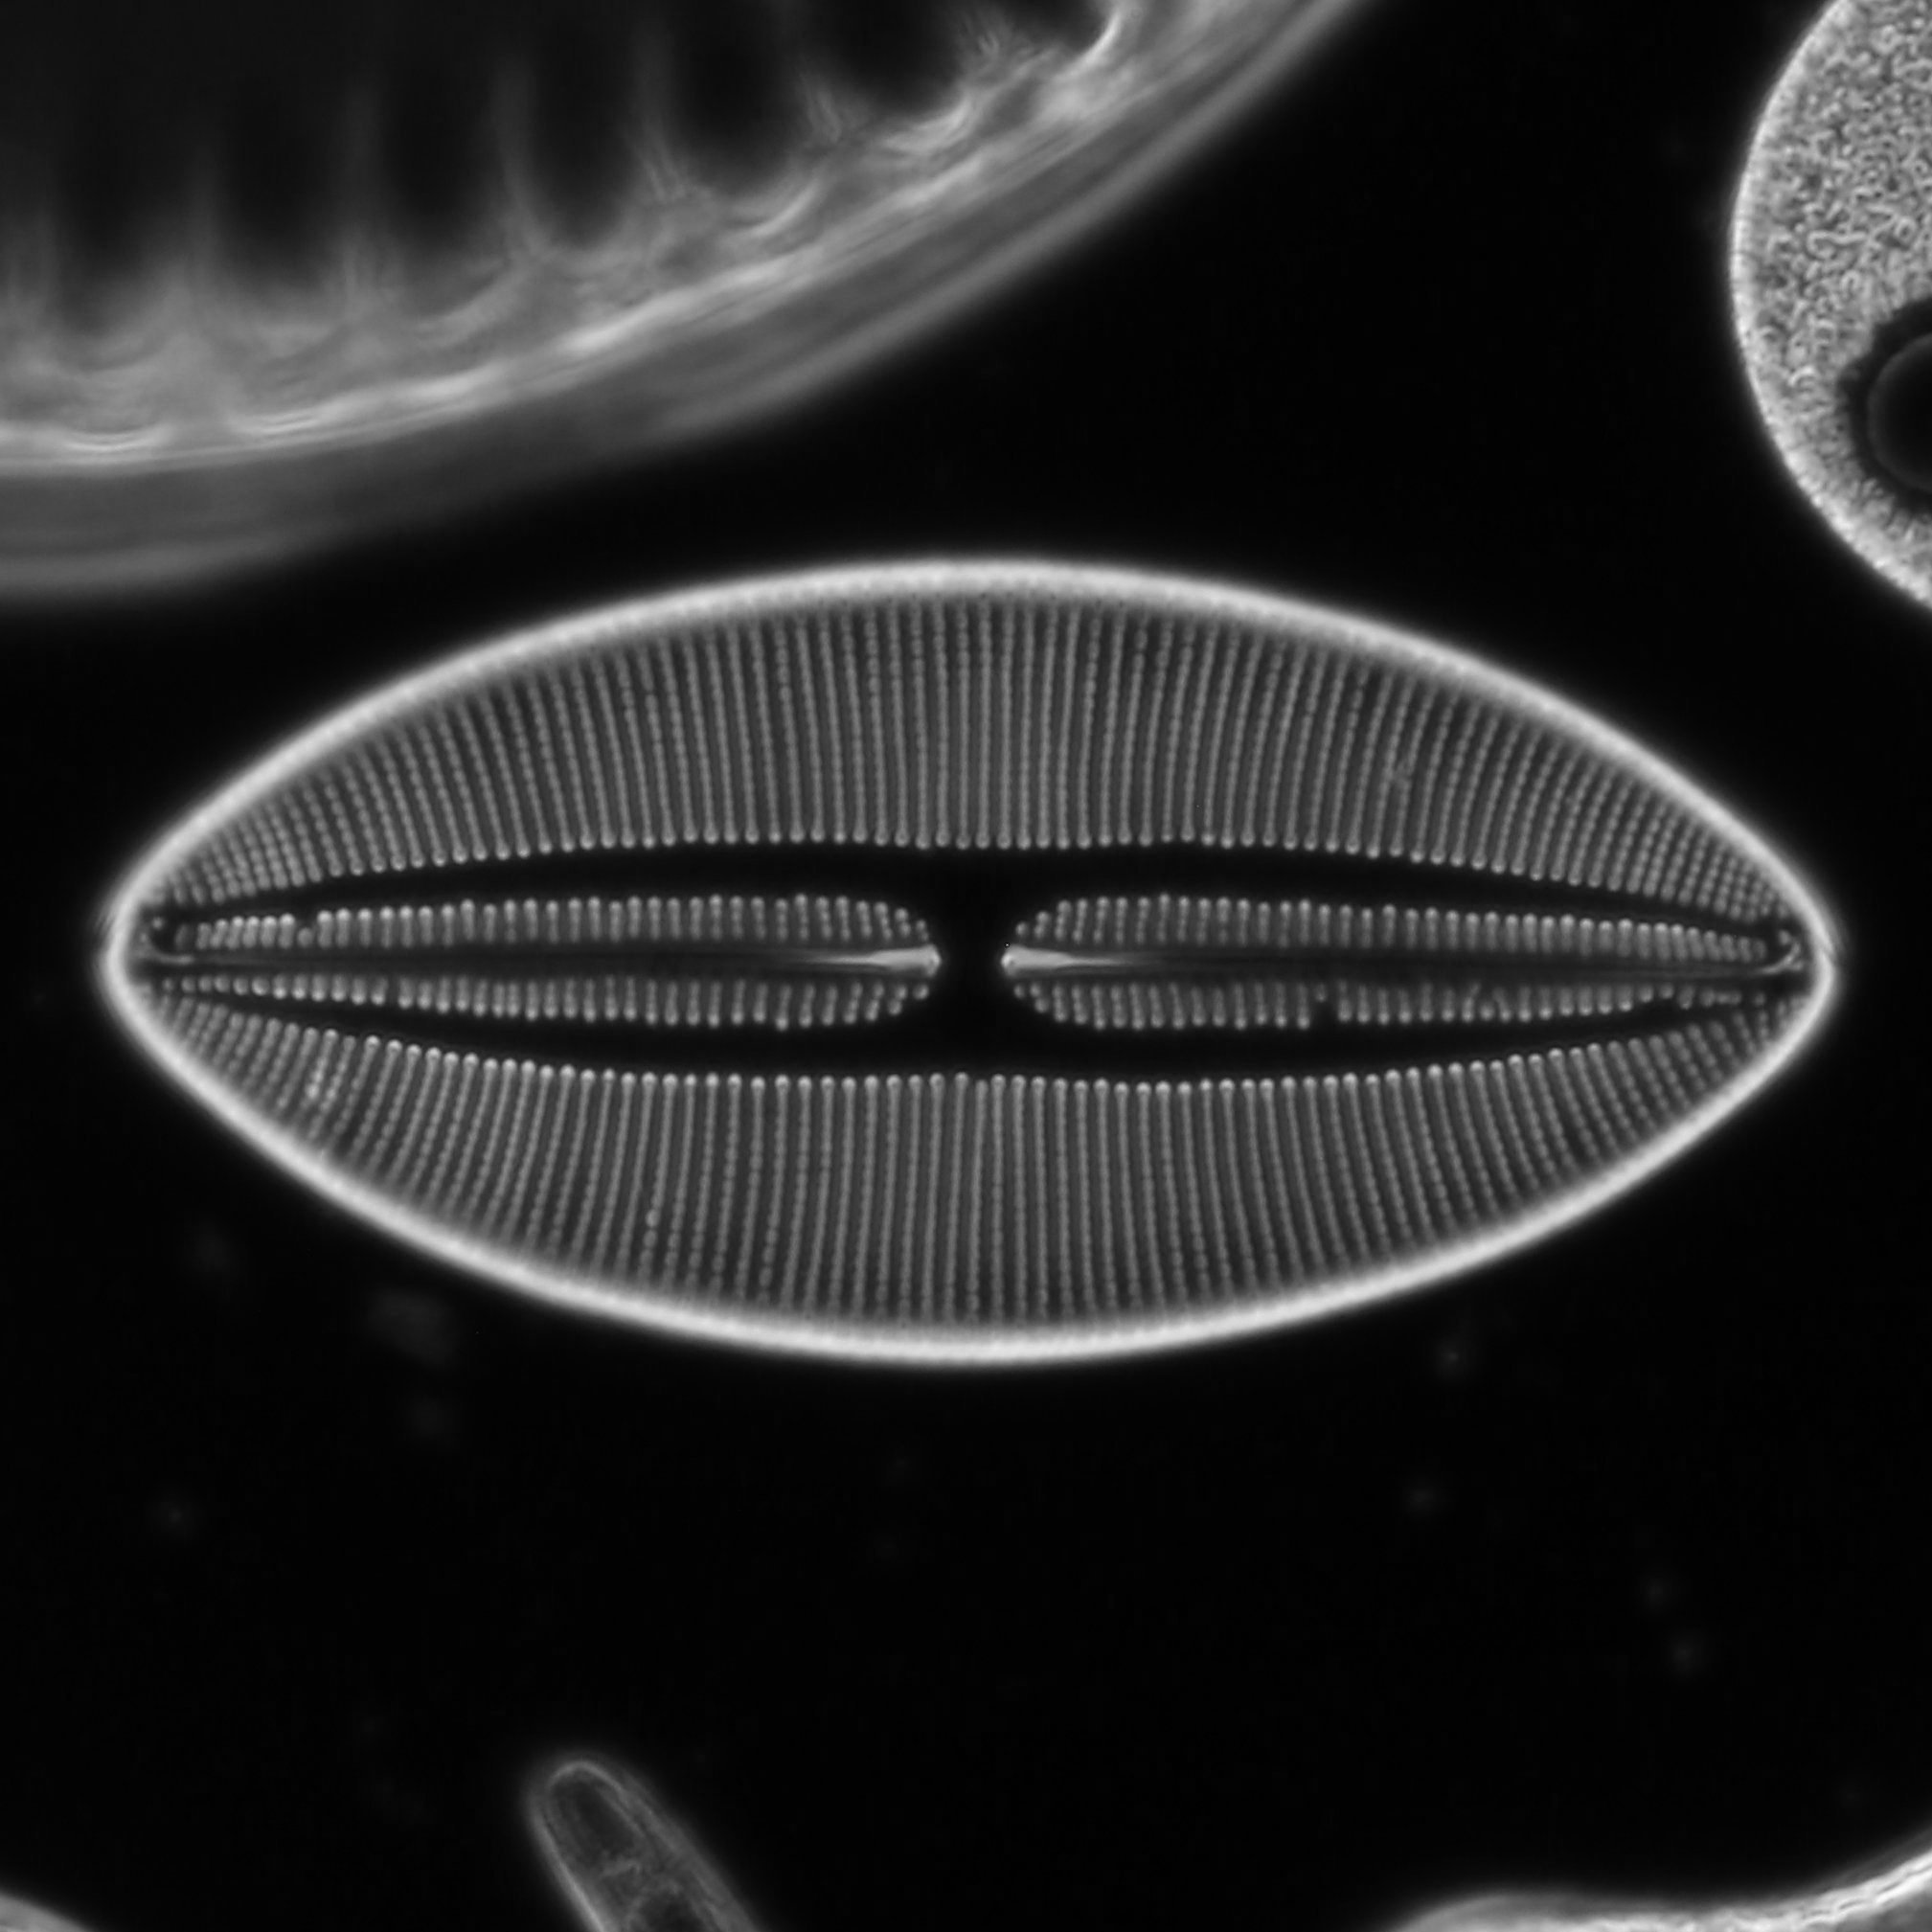
\includegraphics[width=.32\columnwidth]{Exp_2_Microphotography/Figures/5_Diatome_darkfield_05_cropped_32_000norm}} \hspace{0.1mm}
\subfloat[Phase Contrast\label{dphase}]{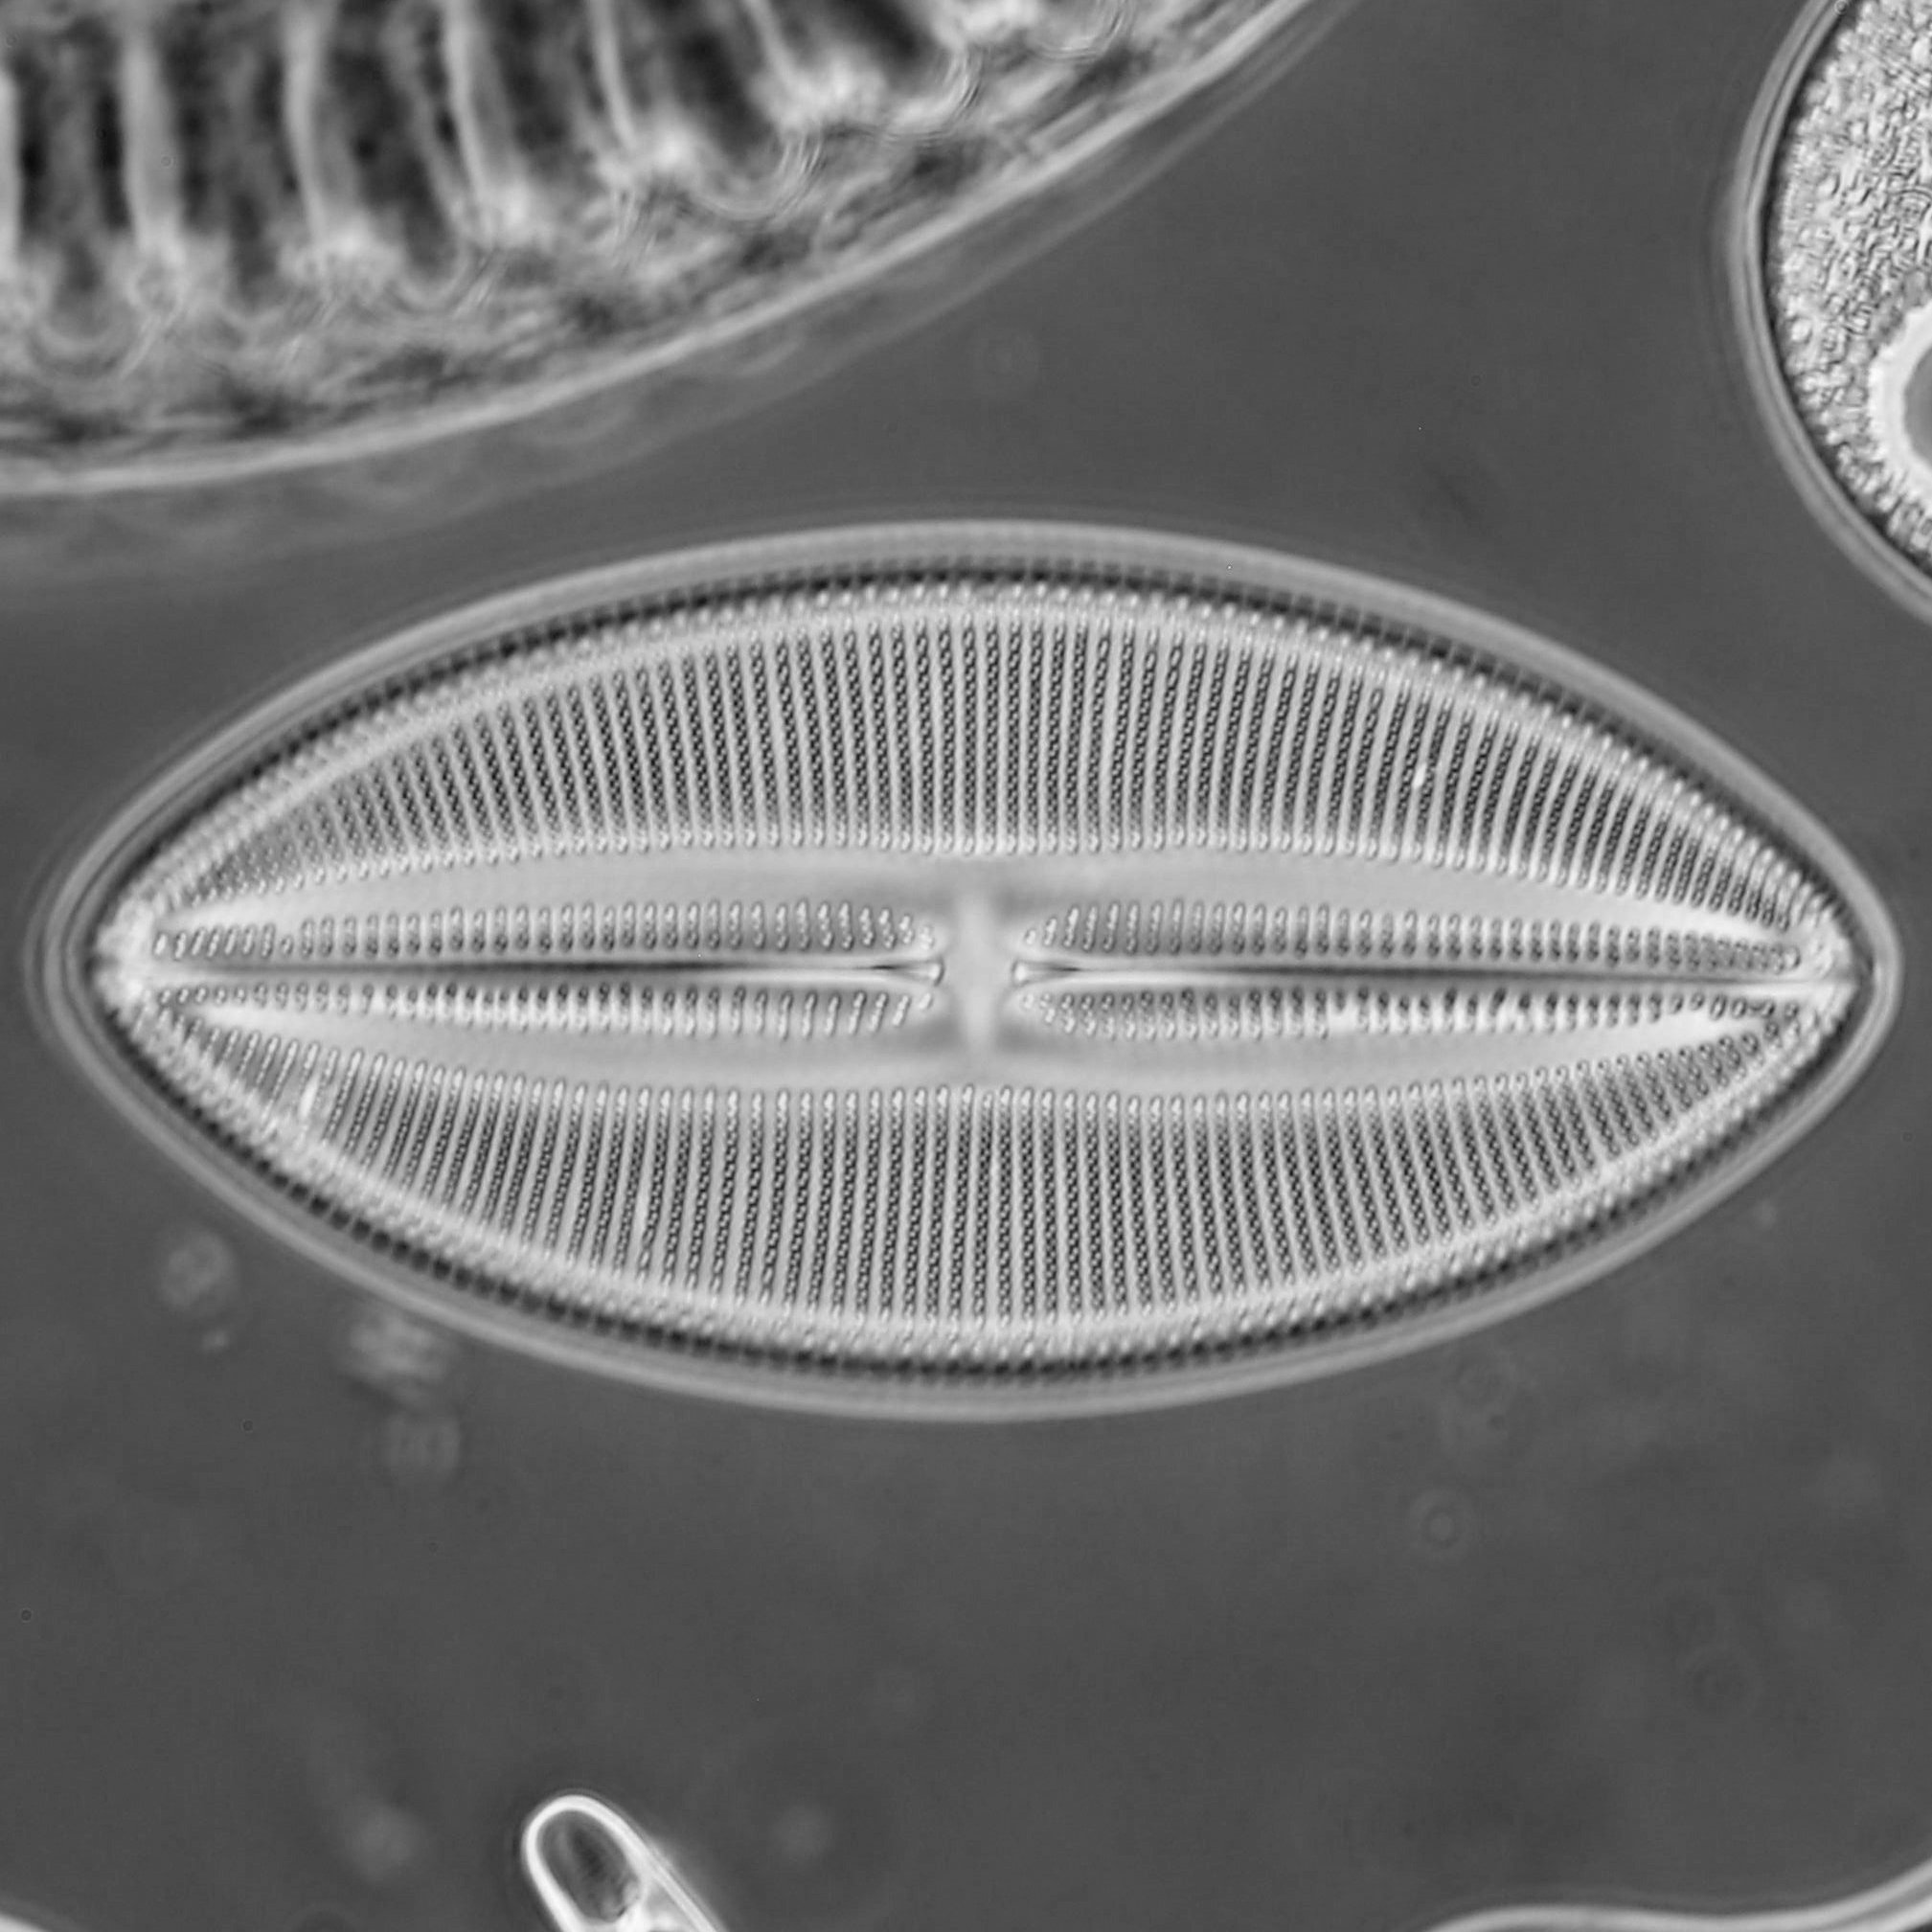
\includegraphics[width=.32\columnwidth]{Exp_2_Microphotography/Figures/27_Diatome_phasecontrast_02_cropped_32_000norm}}\vspace{-0.7em} 
\captionsetup[subfigure]{position=bottom}
\subfloat[Red Filter\label{dred}]{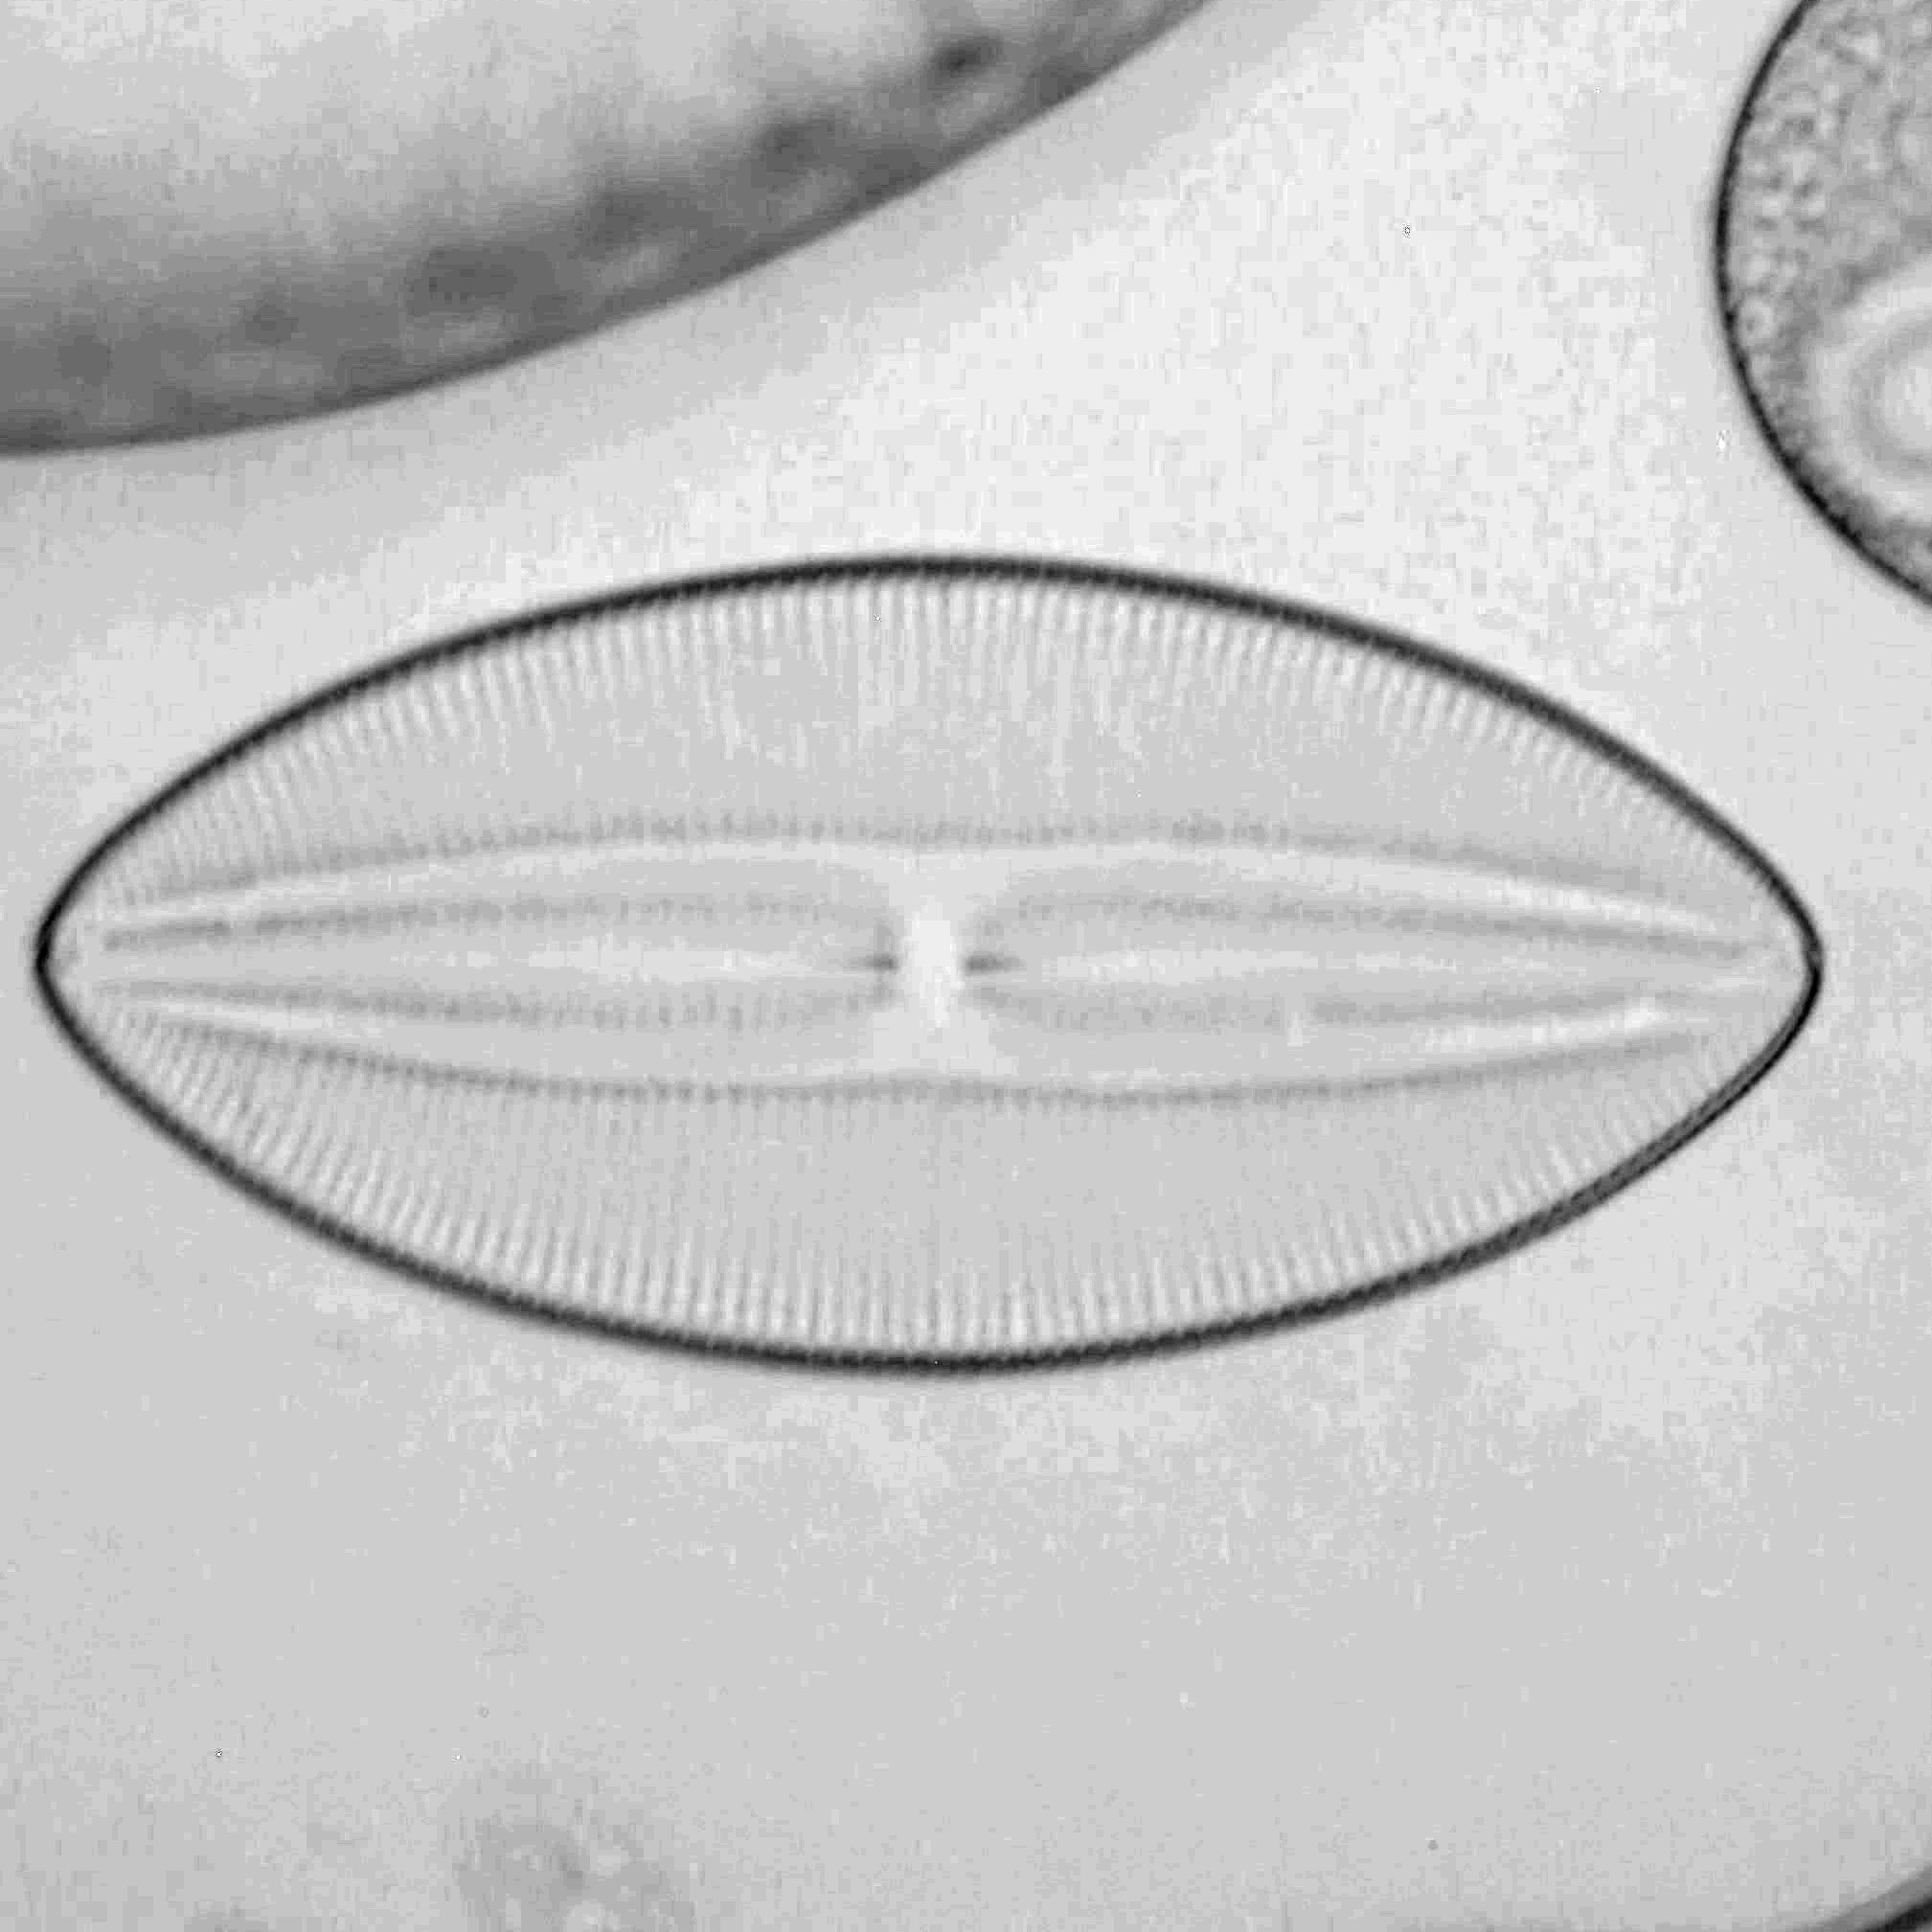
\includegraphics[width=.32\columnwidth]{Exp_2_Microphotography/Figures/13_Diatome_brightfield_redfilter_02_cropped_32_001norm}} \hspace{0.1mm}
\subfloat[Blue Filter\label{dblue}]{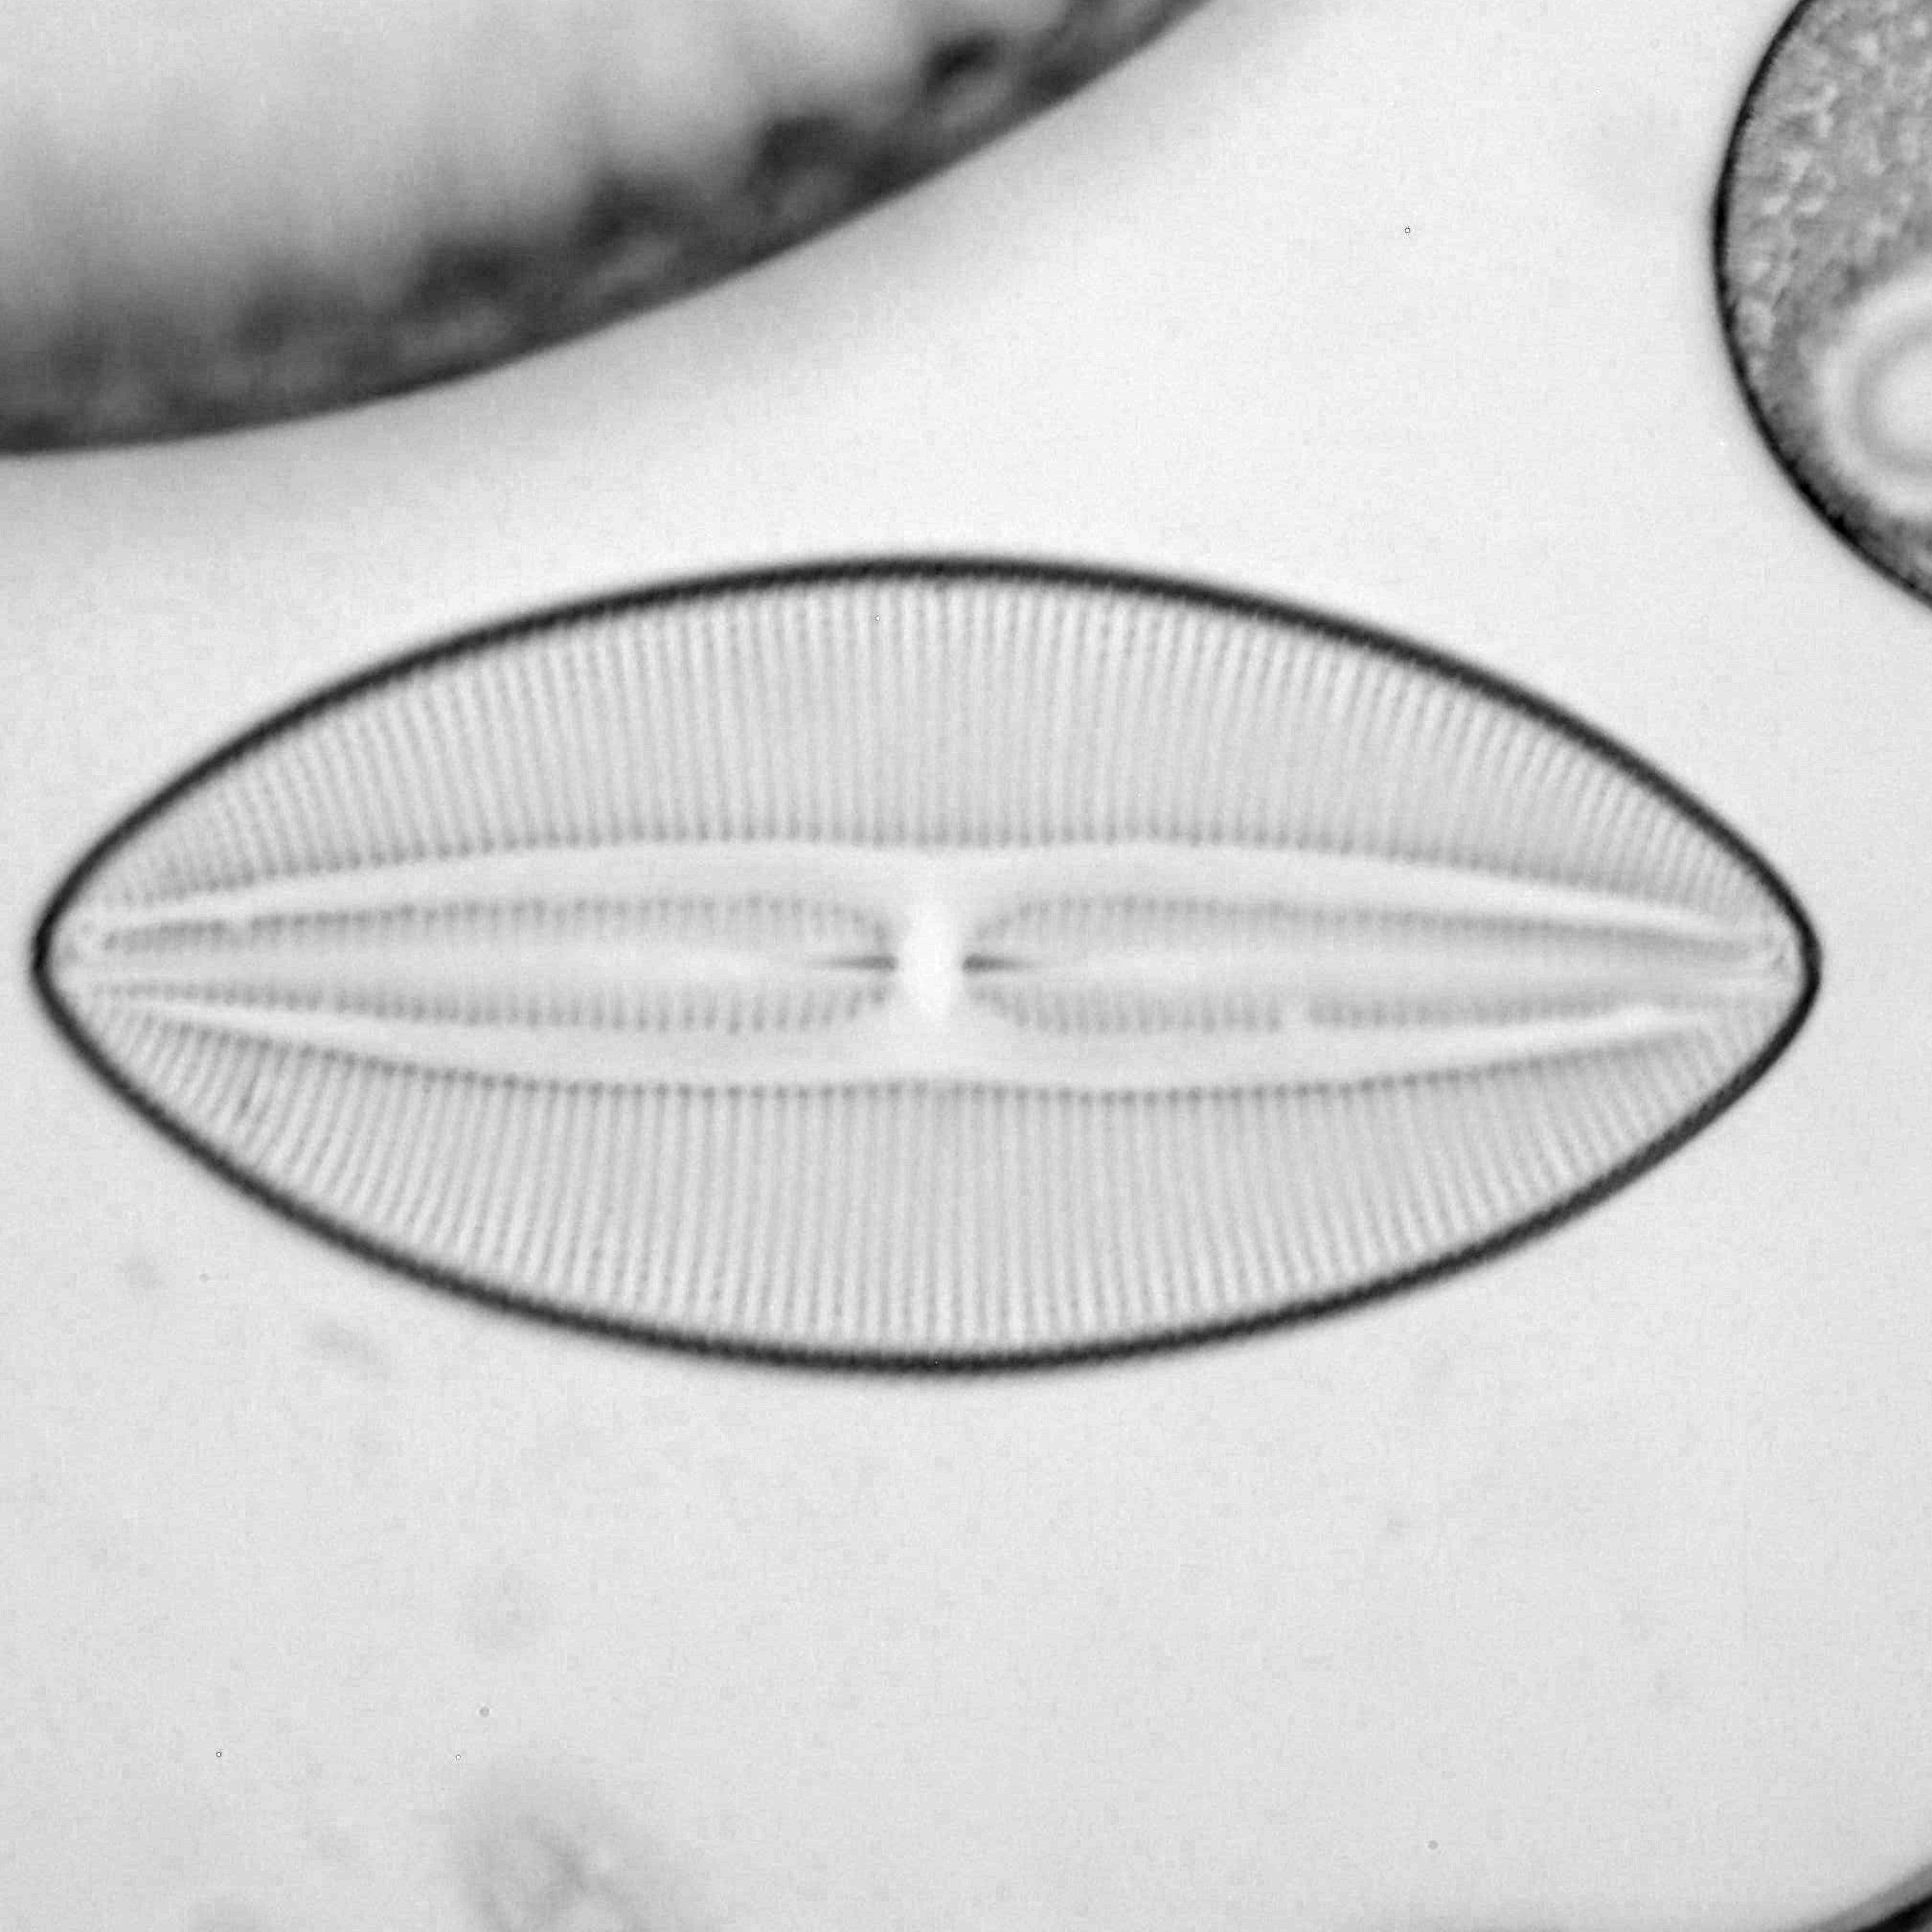
\includegraphics[width=.32\columnwidth]{Exp_2_Microphotography/Figures/14_Diatome_brightfield_bluefilter_02_cropped_32_001norm}} \hspace{0.1mm}
\subfloat[DIC\label{ddic}]{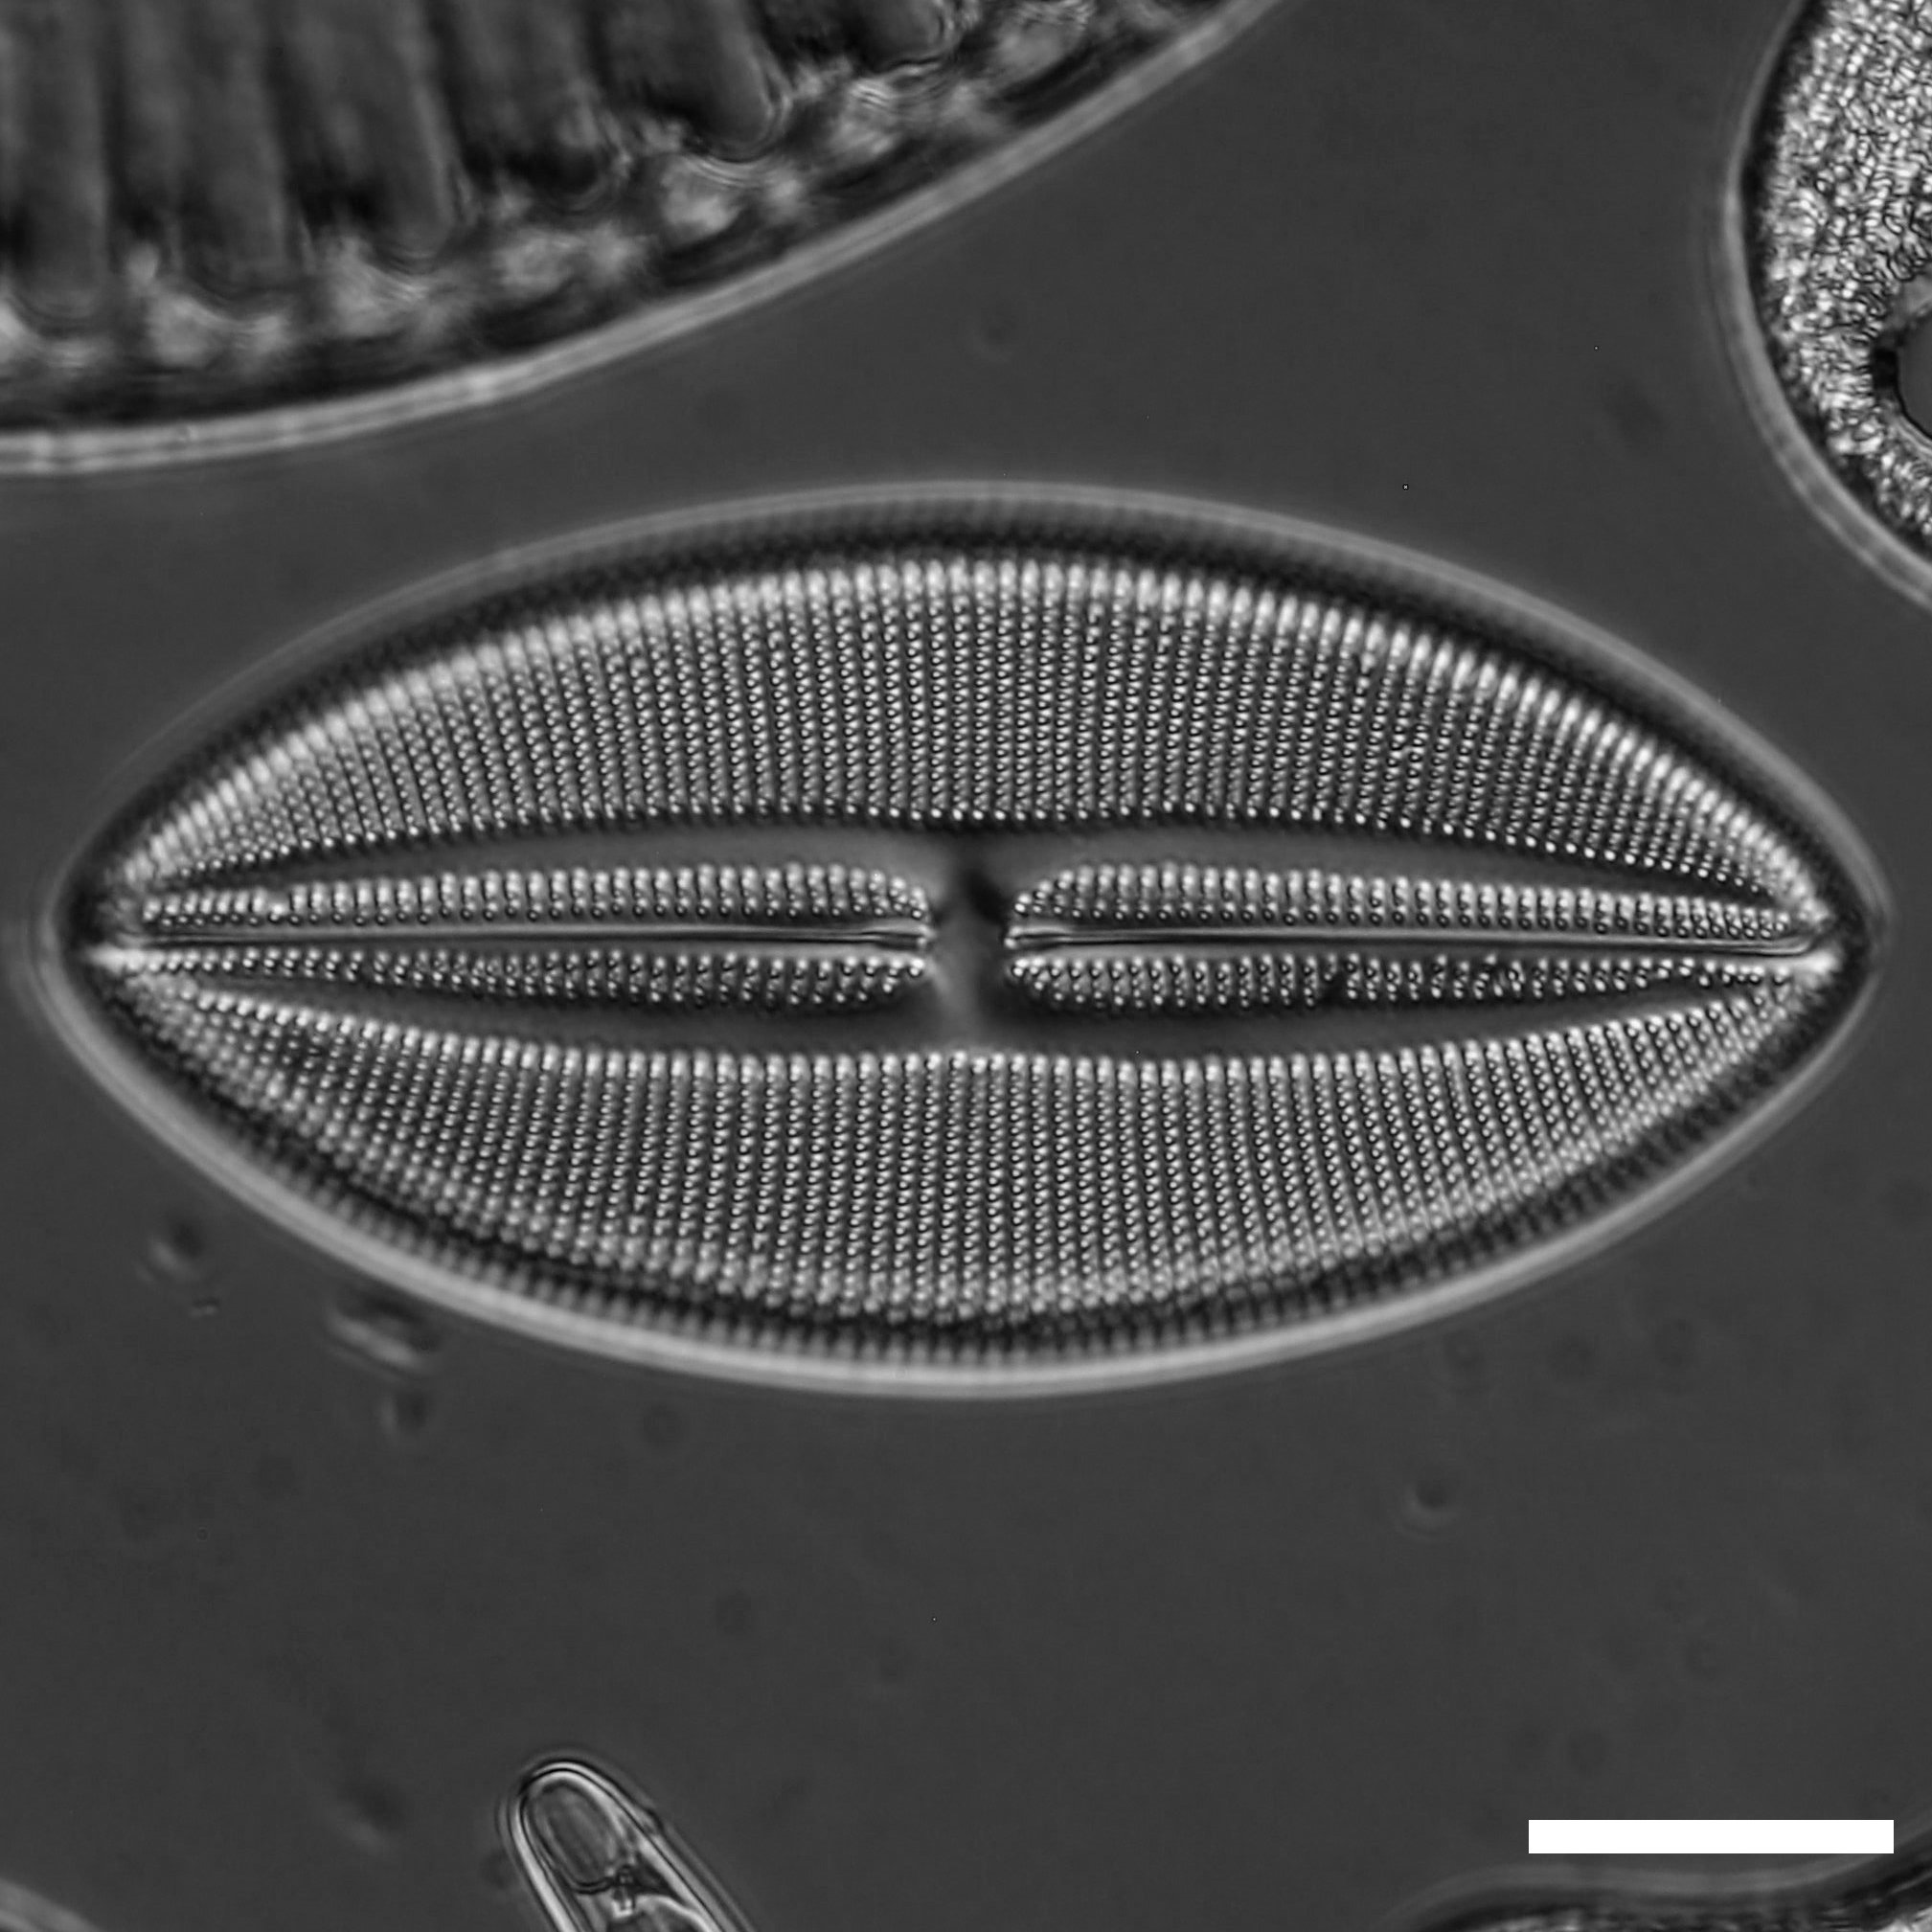
\includegraphics[width=.32\columnwidth]{Exp_2_Microphotography/Figures/30_Diatome_DIC_03_cropped_32_000norm_scale25}}
\caption[Clockwise from top left:bright,dark,pc,blue,red,dic]{Comparison of diatom (\textit{N. lyra}) images using brightfield, darkfield, phase contast, and DIC microscopy. 
Additionally, brightfield microscopy was also conducted using blue and red filters. 
A, C, D, E, and F used Plan Neofluar 40$\times$/0.75 Ph2 lens, B used Achroplan 40$\times$/0.6 Korr lens. 
Scalebar is 25 $\mu$m.} 
\label{fig:diatomes}
\end{figure}

Fig.~\ref{fig:diatomes} shows images of a diatom (\textit{Navicula lyra}) taken with different techniques. 
As can be seen in the Fig.~\ref{dred} \&~\ref{dblue}, the resulting images look comparatively grainy. 
Normalization without saturation of the grey-scaled images performed poorly due to outliers for both these images. 
Therefore, saturation was set to 0.01\% to improve the contrast, though graininess was then introduced to the image. 
However, also apparent in these images, that light with longer wavelength (e.g. red light, Fig.~\ref{dred}) does not show minute structures of the diatom well, in comparison to blue light (Fig.~\ref{dblue}) which has shorter wavelength. 
The shorter wavelength of blue light are scattered more strongly by smaller structures (or particles) than the longer wavelength red light, hence the less obvious structures of the diatom when viewed with red light/filter. 
Both of these lights compose the light for brightfield microscopy (Fig.~\ref{dbright}), which gives just as detailed an image as its is for darkfield microscopy (Fig.~\ref{ddark}), just inversely illuminated. 
However, the darkfield images are arguably advantageous in this case due to the fact that since the specimen is unstained, more contrast can be obtained this way in comparison to brightfield microscopy. 
Other methods to obtain even more contrast were also performed, namely; phase contrast microscopy, whose image in Fig.~\ref{dphase} shows a glowing halo around the specimen, and DIC - Differential Interference Contrast (Fig.~\ref{ddic}) which displays the characteristic pseudo-3D effect.

It can also be illustrated by this specimen the effect of NA on resolution. 
Fig.~\ref{fig:NA} shows how the minute structures are more easily resolved by higher NA lenses. 
Although the techniques used are different, but the effect can still be clearly observed \cite{North2006}.

\begin{figure}[h]
\centering
\subfloat[NA = 0.6 \label{insdark}]{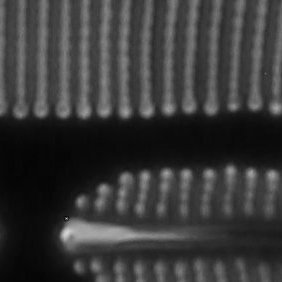
\includegraphics[width=.32\columnwidth]{Exp_2_Microphotography/Figures/inset5_Diatome_darkfield_05_cropped_32_000norm-1}} \hspace{0.1mm}
\subfloat[NA =  0.75 \label{insphase}]{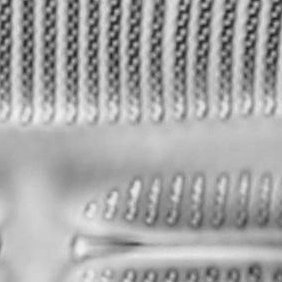
\includegraphics[width=.32\columnwidth]{Exp_2_Microphotography/Figures/inset27_Diatome_phasecontrast_02_cropped_32_000norm-1}} \hspace{0.1mm}
\subfloat[NA = 0.75 \label{insdic}]{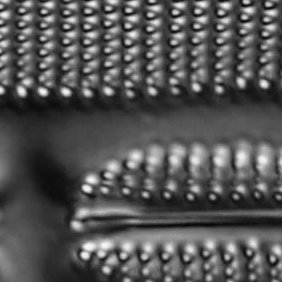
\includegraphics[width=.32\columnwidth]{Exp_2_Microphotography/Figures/inset30_Diatome_DIC_03_cropped_32_000norm}}
\caption{Comparison of the effect of different NA on resolution. 
Zoomed in images of the same diatom specimen. 
A used Achroplan 40$\times$/0.6 Korr lens, B and C used Plan Neofluar 40$\times$/0.75 Ph2 lens. 
No scale bar presented, images are for illustrative purposes only.}
\label{fig:NA}
\end{figure}

%-----------------------------------
\subsection{Bloodsmear}

\begin{figure}[h!]
\centering
\captionsetup[subfigure]{position=bottom}
\subfloat[Brightfield\label{bbright}]{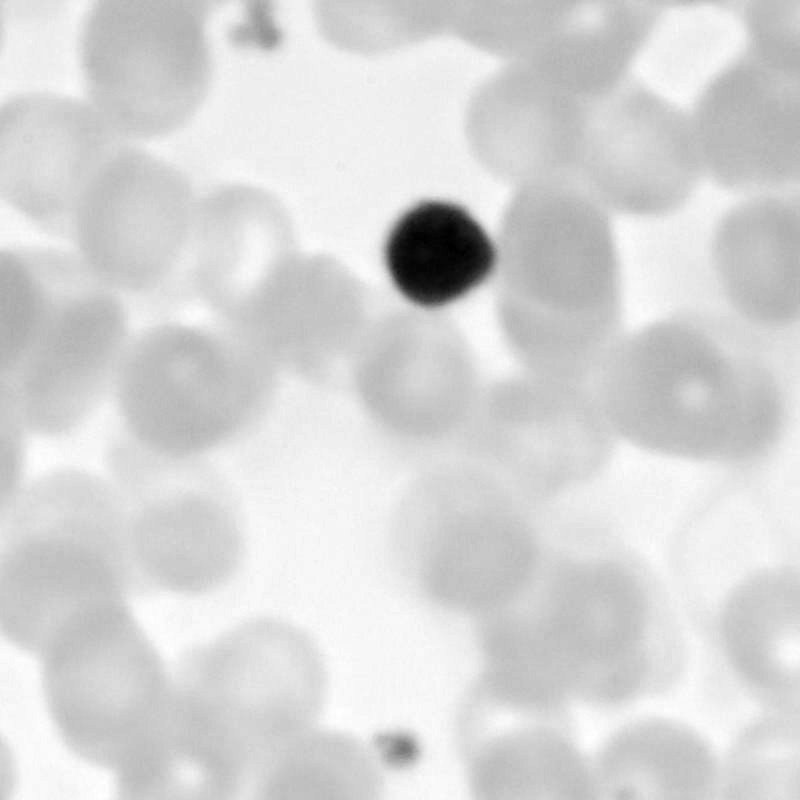
\includegraphics[width=.24\columnwidth]{Exp_2_Microphotography/Figures/Bloodsorted/Bloodsmear_brightfield_02--800crop_32bit_0.01ecandnorm}}\hspace{0.1mm}
\subfloat[Darkfield\label{bdark}]{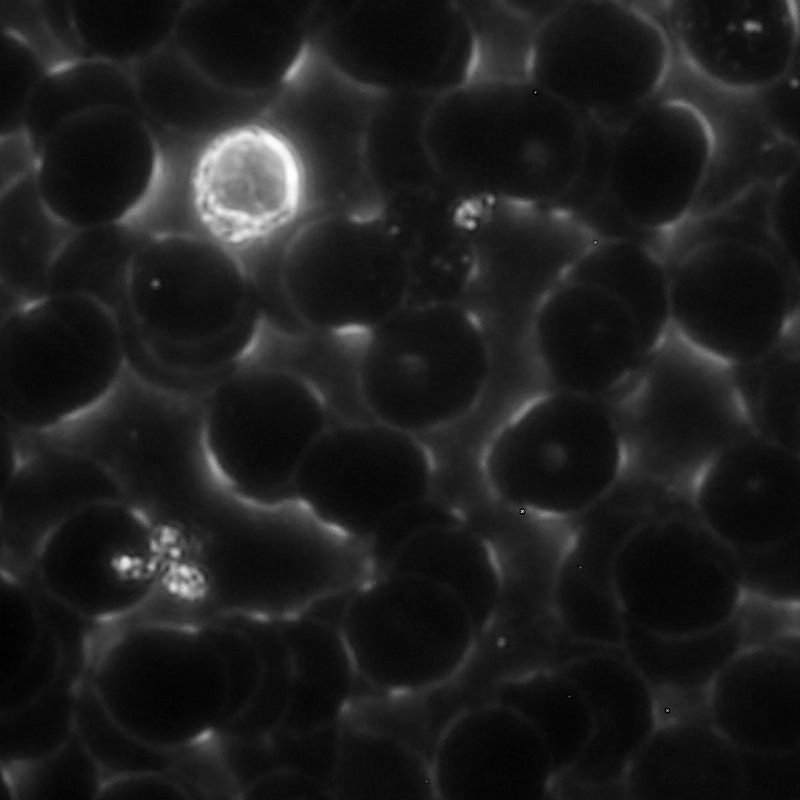
\includegraphics[width=.24\columnwidth]{Exp_2_Microphotography/Figures/Bloodsorted/Bloodsmear_darkfield_07-1--800crop_32bit_0.01ecandnorm}}\hspace{0.1mm}
%\captionsetup[subfigure]{position=bottom}
\subfloat[Phase Contrast\label{bphase}]{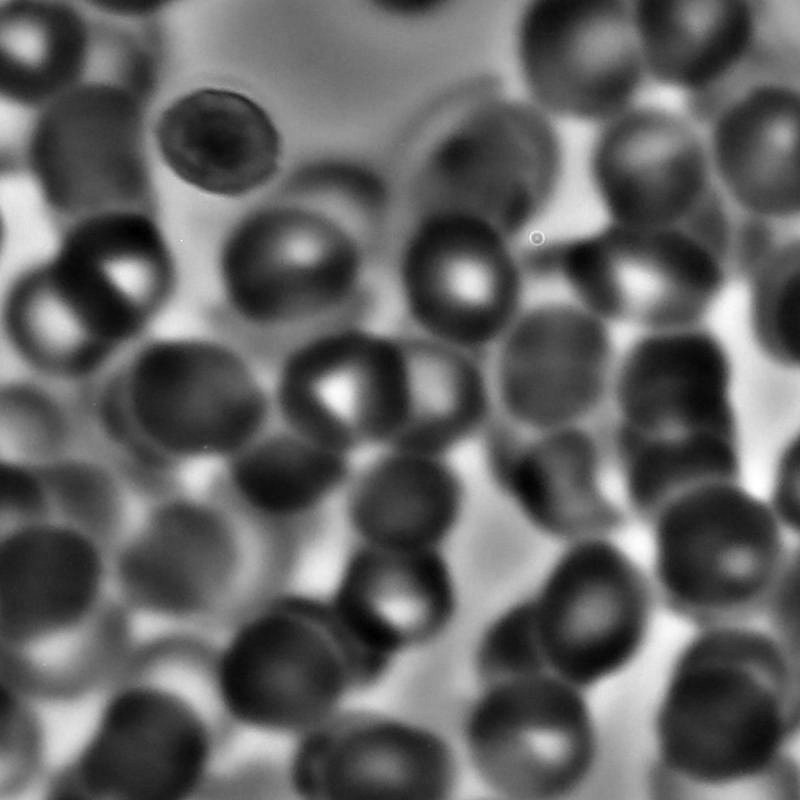
\includegraphics[width=.24\columnwidth]{Exp_2_Microphotography/Figures/Bloodsorted/Bloodsmear_phasecontrast_01-1--800crop_32bit_0.01ecandnorm}}\hspace{0.1mm}
\subfloat[DIC\label{bdic}]{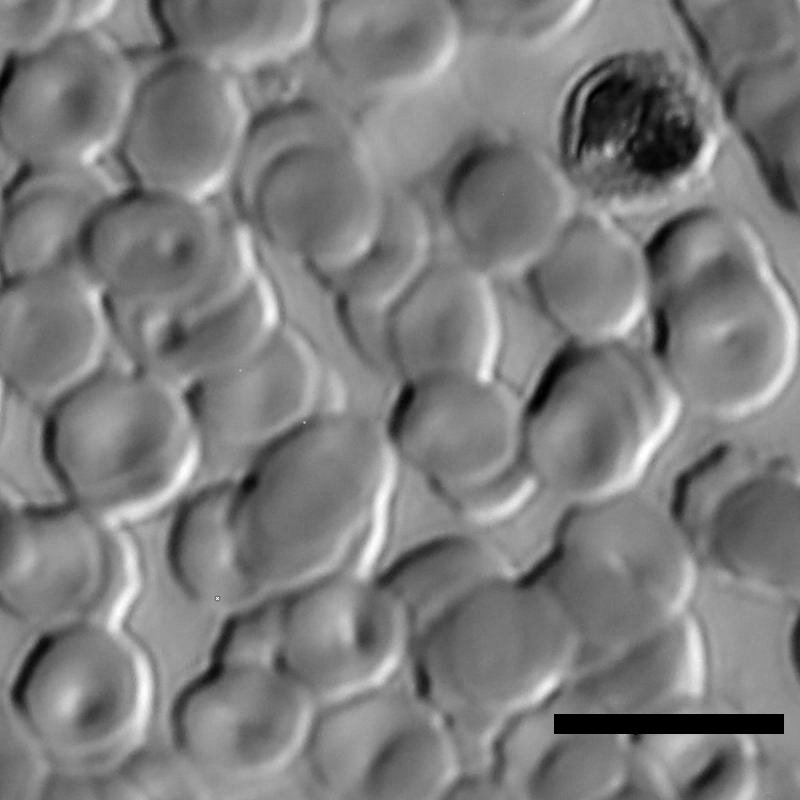
\includegraphics[width=.24\columnwidth]{Exp_2_Microphotography/Figures/Bloodsorted/Bloodsmear_DIC_02--800crop_32bit_ecandnorm_15umblack}}\\
\caption{Bloodsmear specimen under brightfield, darkfield, phase contrast, and DIC microscopy. 
A, C, and D used Plan Neofluar 40$\times$/0.75 Ph2 lens, B used Achroplan 40$\times$/0.6 Korr lens. 
Scalebar is 15 $\mu$m.} 
\label{fig:blood}
\end{figure}

In the bloodsmear specimen, all imaging methods (Fig.~\ref{fig:blood}) could help distinguish red blood cells among white blood cells. 
The darkfield image (Fig.~\ref{bdark}) seems to display this most prominently, other than the fact that the contrast between the background and other cells looks very poor. 
The phase contrast and DIC (Fig.~\ref{bphase} \&~\ref{bdic}) method allow a better resolution of the cells between each other and also against the background in comparison to the brightfield (Fig.~\ref{bbright}) and darkfield microscopy. 

%---------------------------------------------------
\subsection{Blowfly salivary gland}

\begin{figure}[h]
\centering
\captionsetup[subfigure]{position=top}
\subfloat[Septate Junctions\label{bsred}]{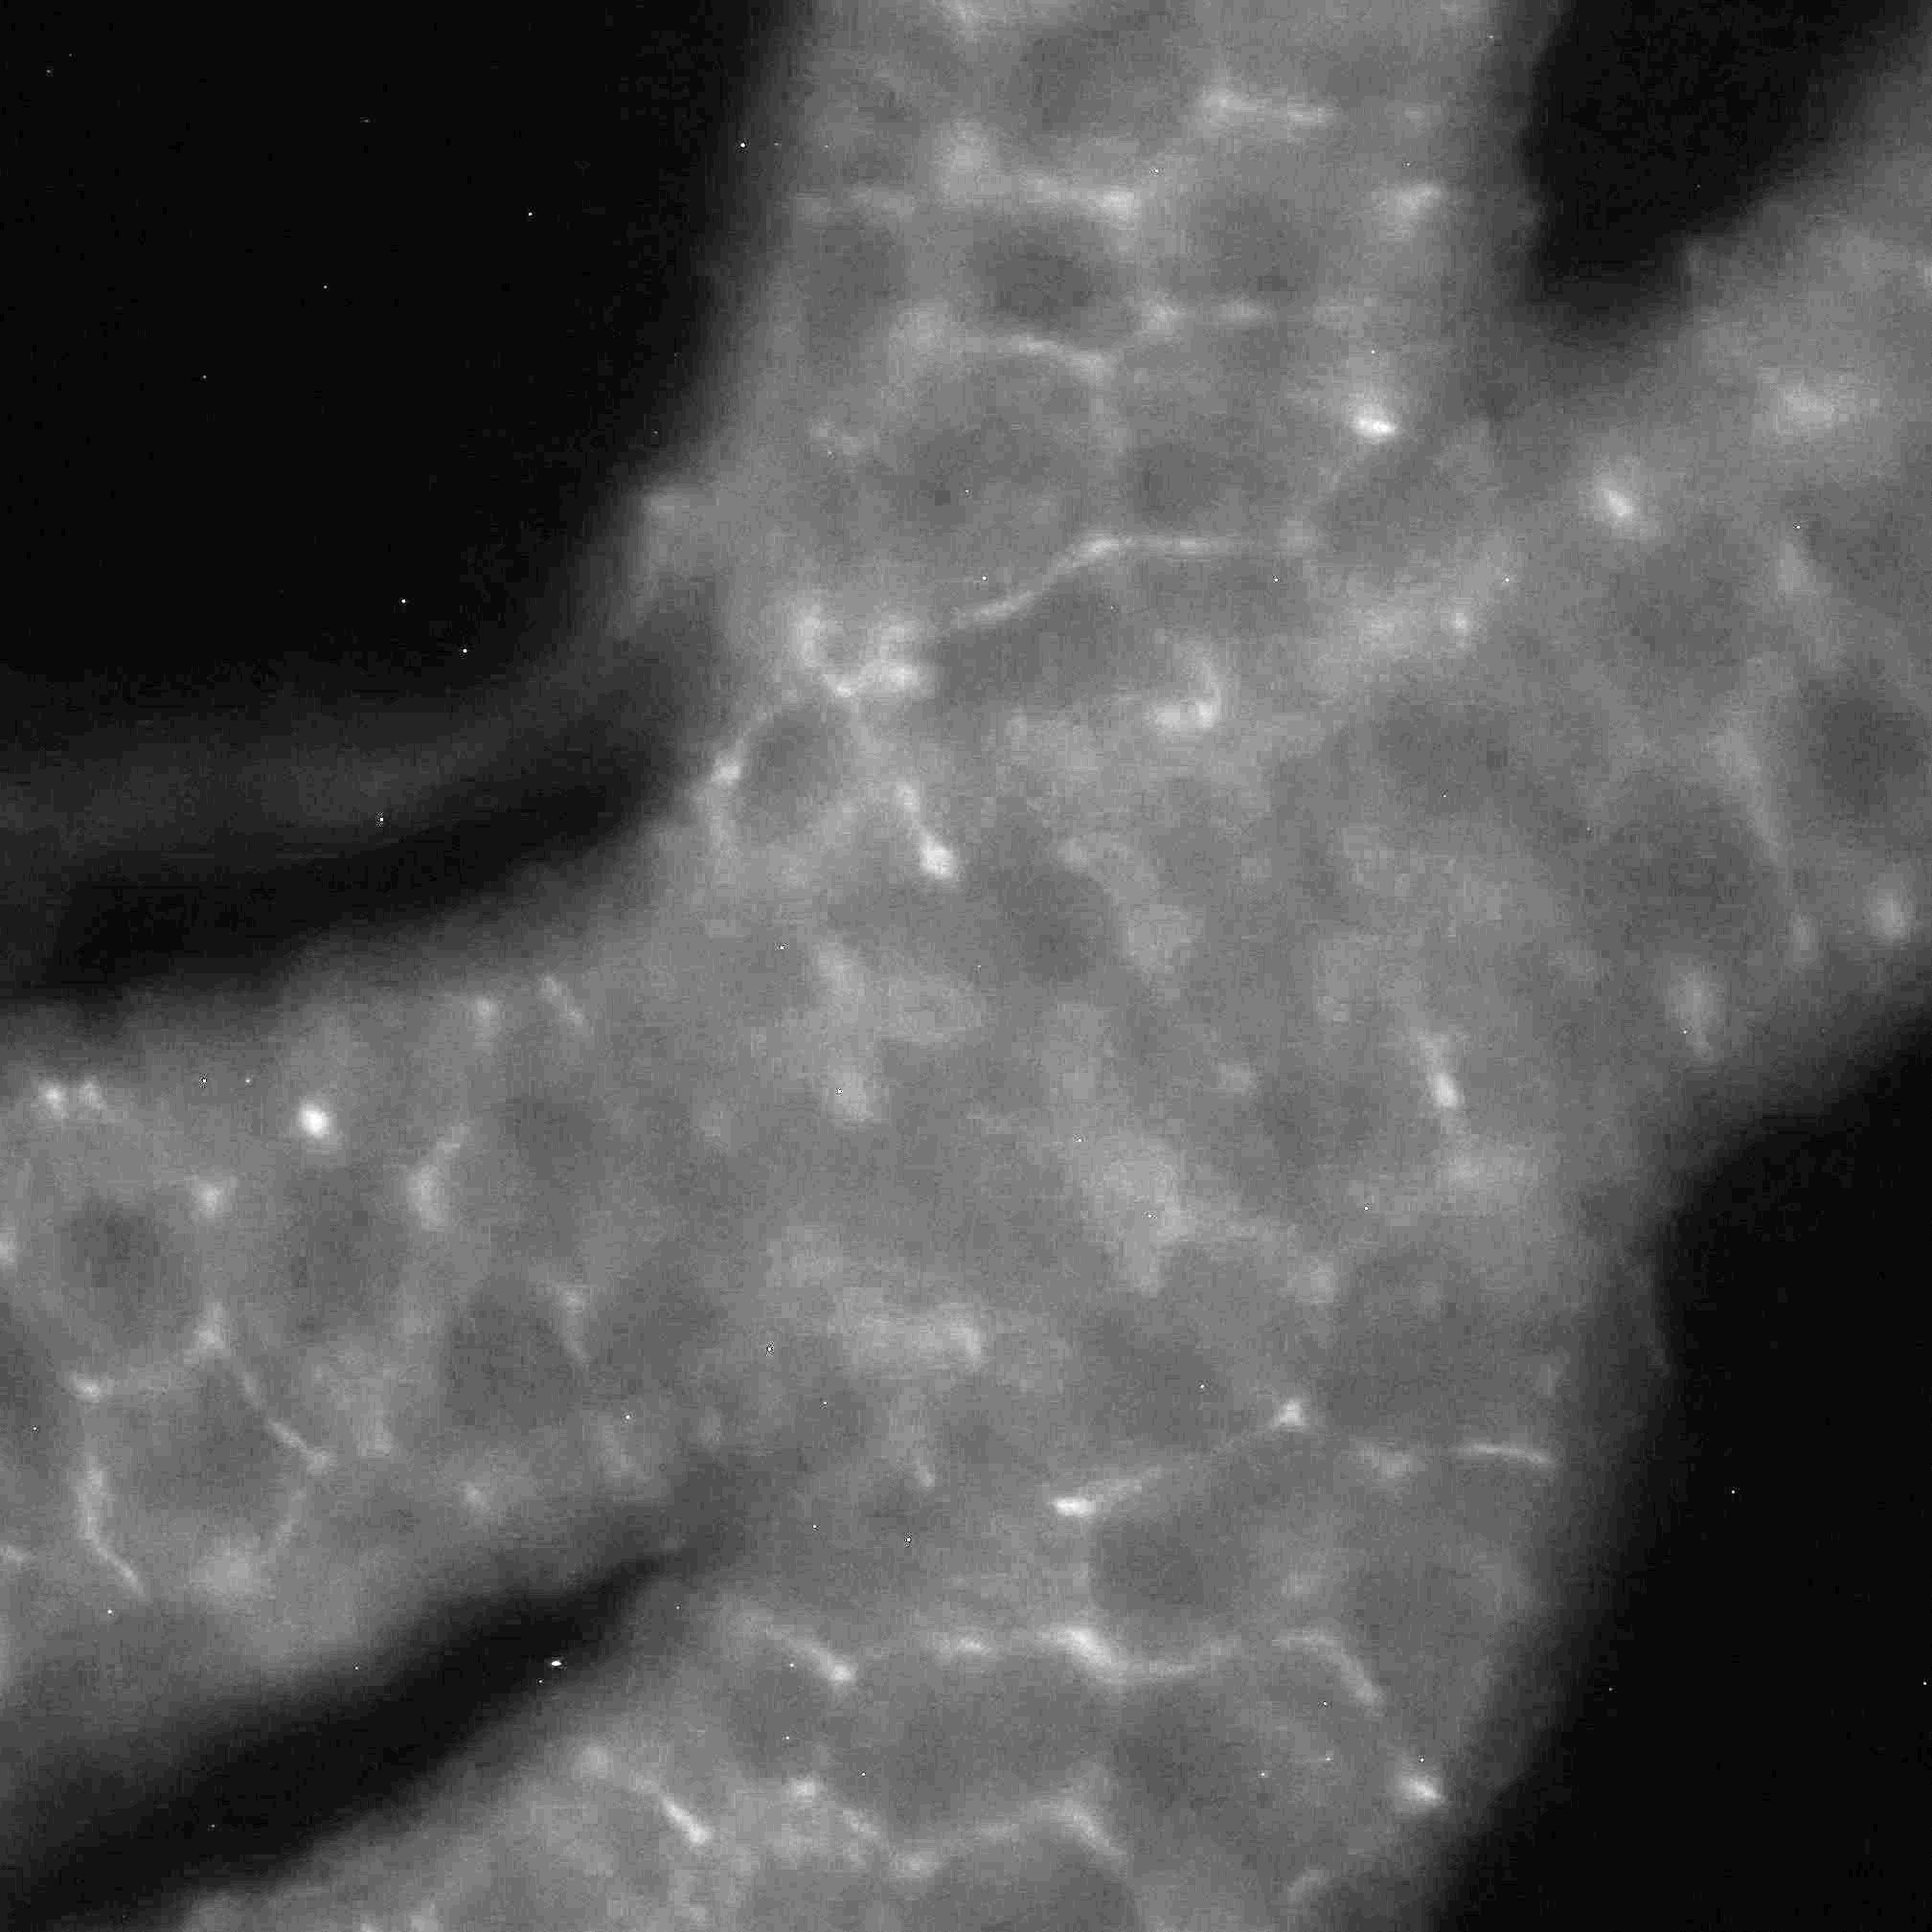
\includegraphics[width=.3\columnwidth]{Exp_2_Microphotography/Figures/35_Blowfly_Fluorescence_03_red_cropped_32_001norm}} \hspace{0.1mm}
\subfloat[Actin\label{bsgreen}]{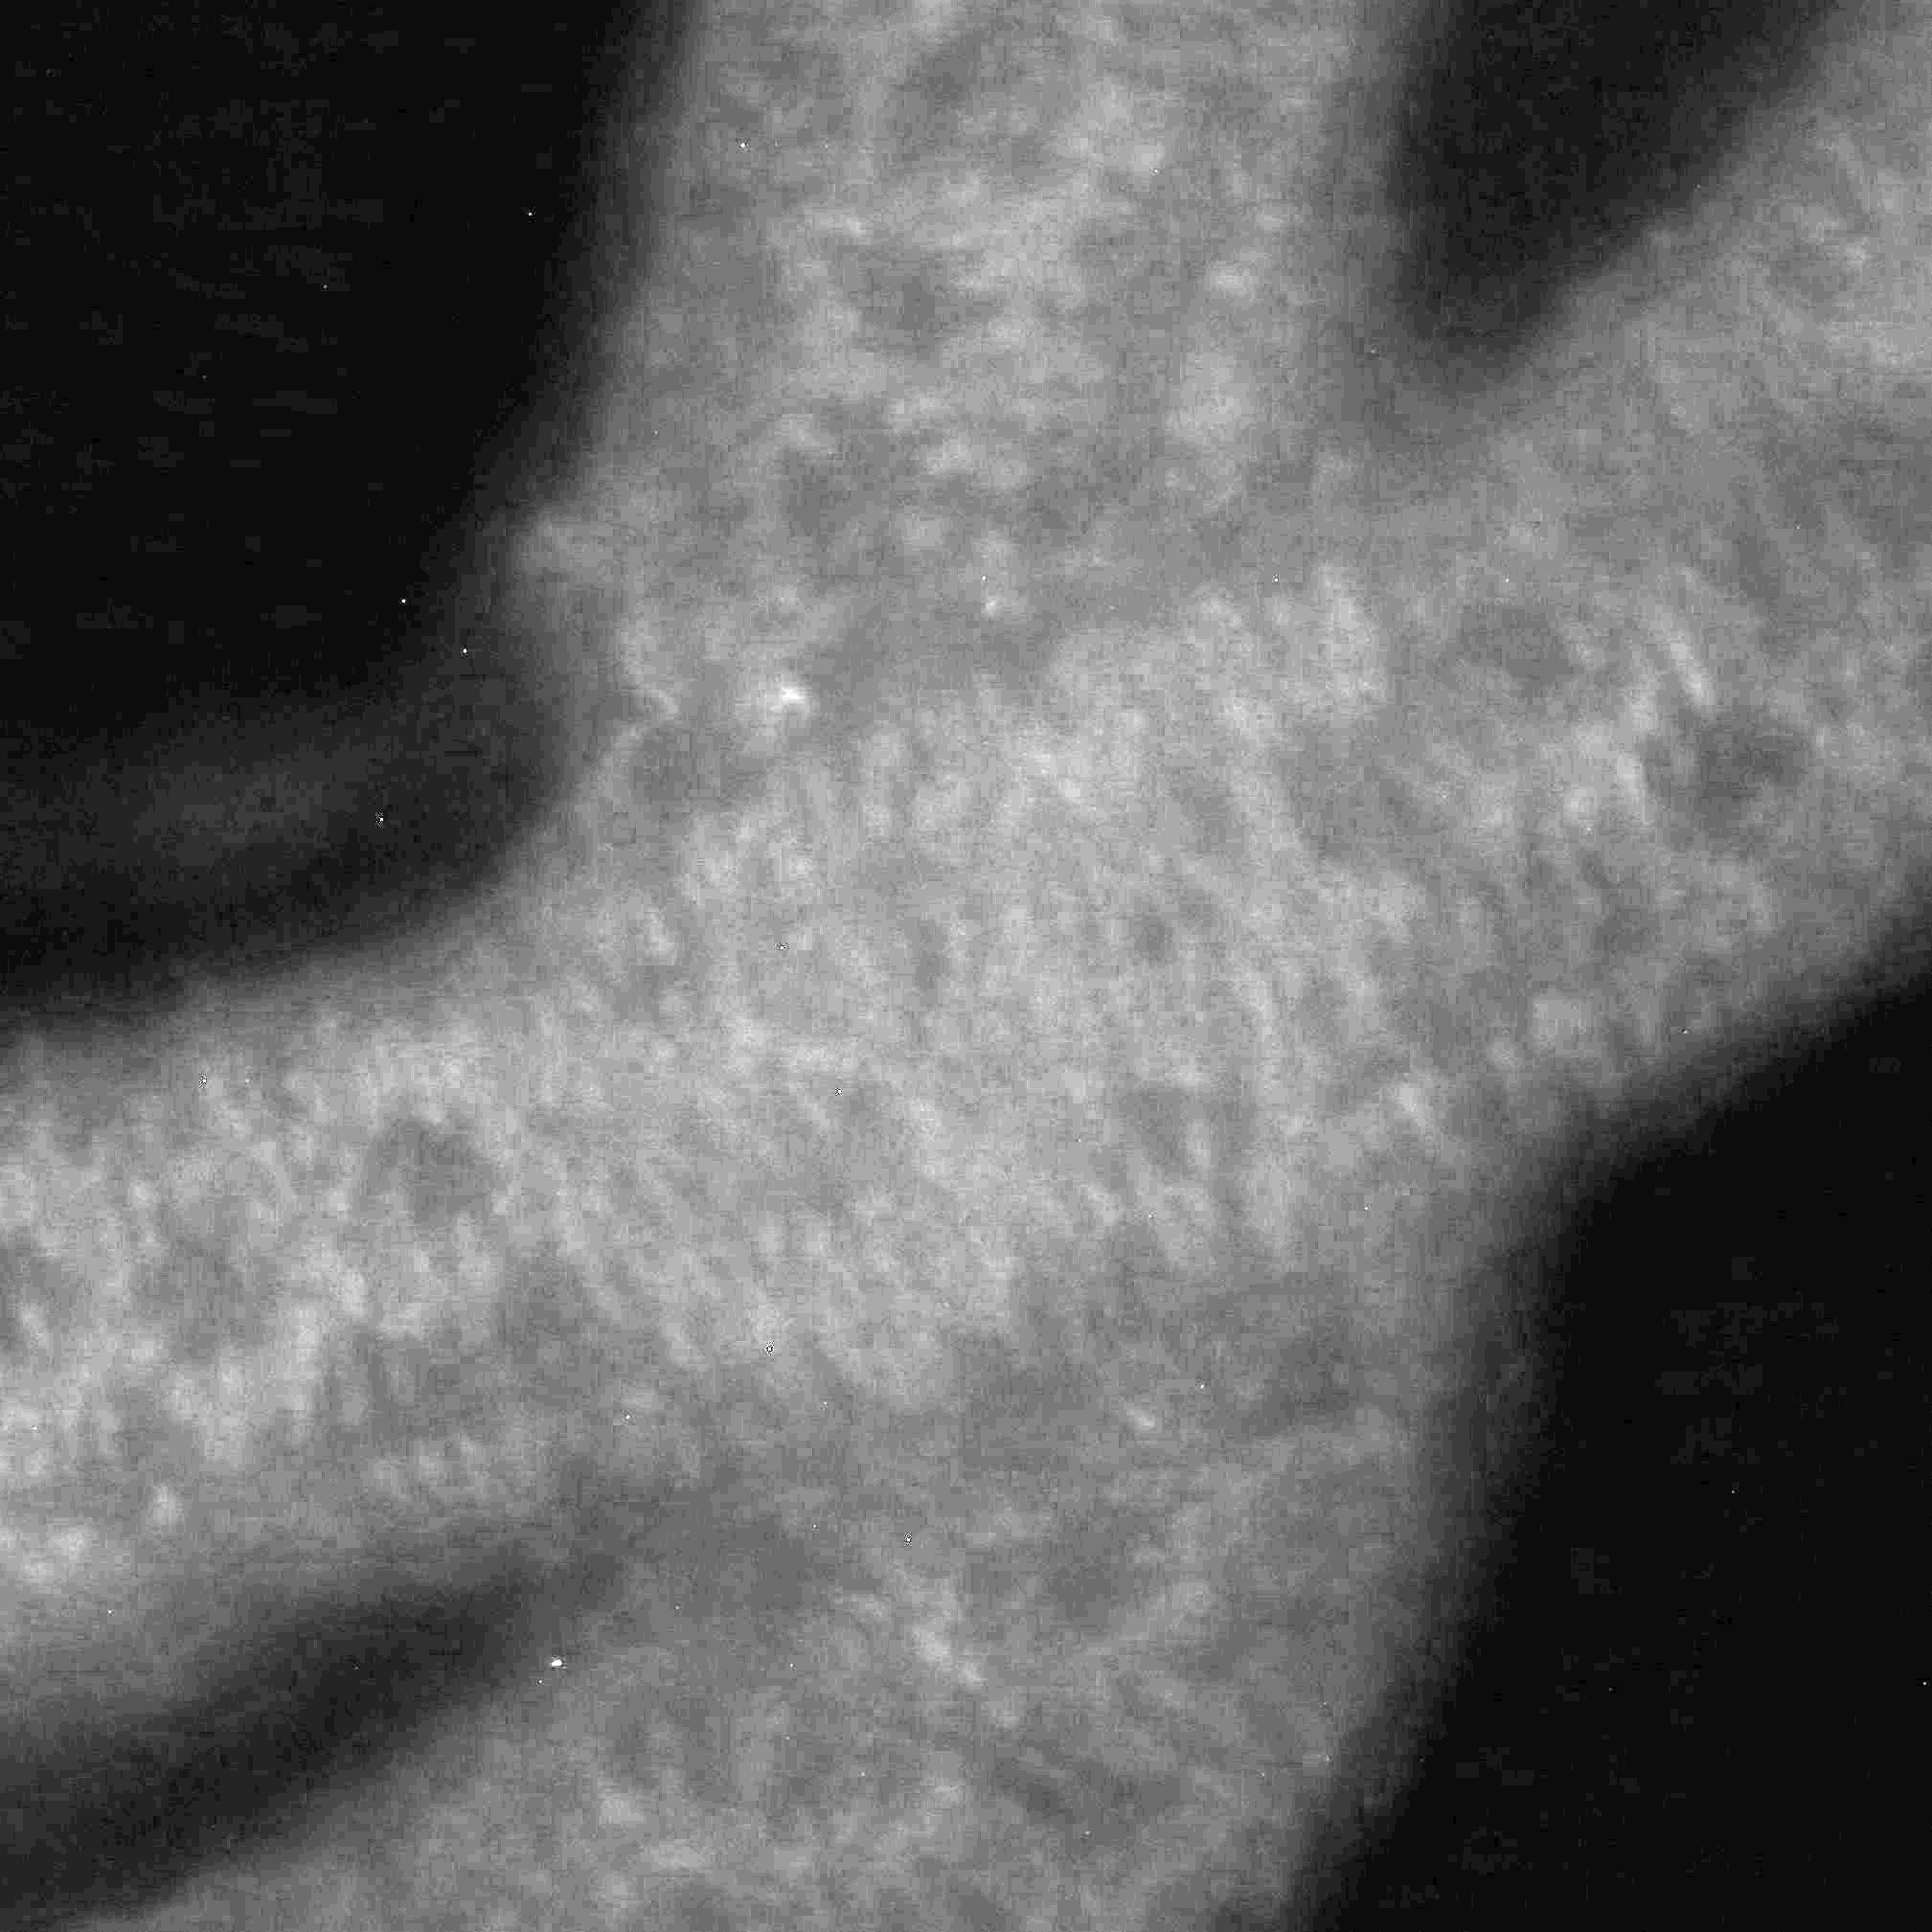
\includegraphics[width=.3\columnwidth]{Exp_2_Microphotography/Figures/34_Blowfly_Fluorescence_02_green_cropped_32_001norm}}\hspace{0.1mm}
\subfloat[Nucleus\label{bsblue}]{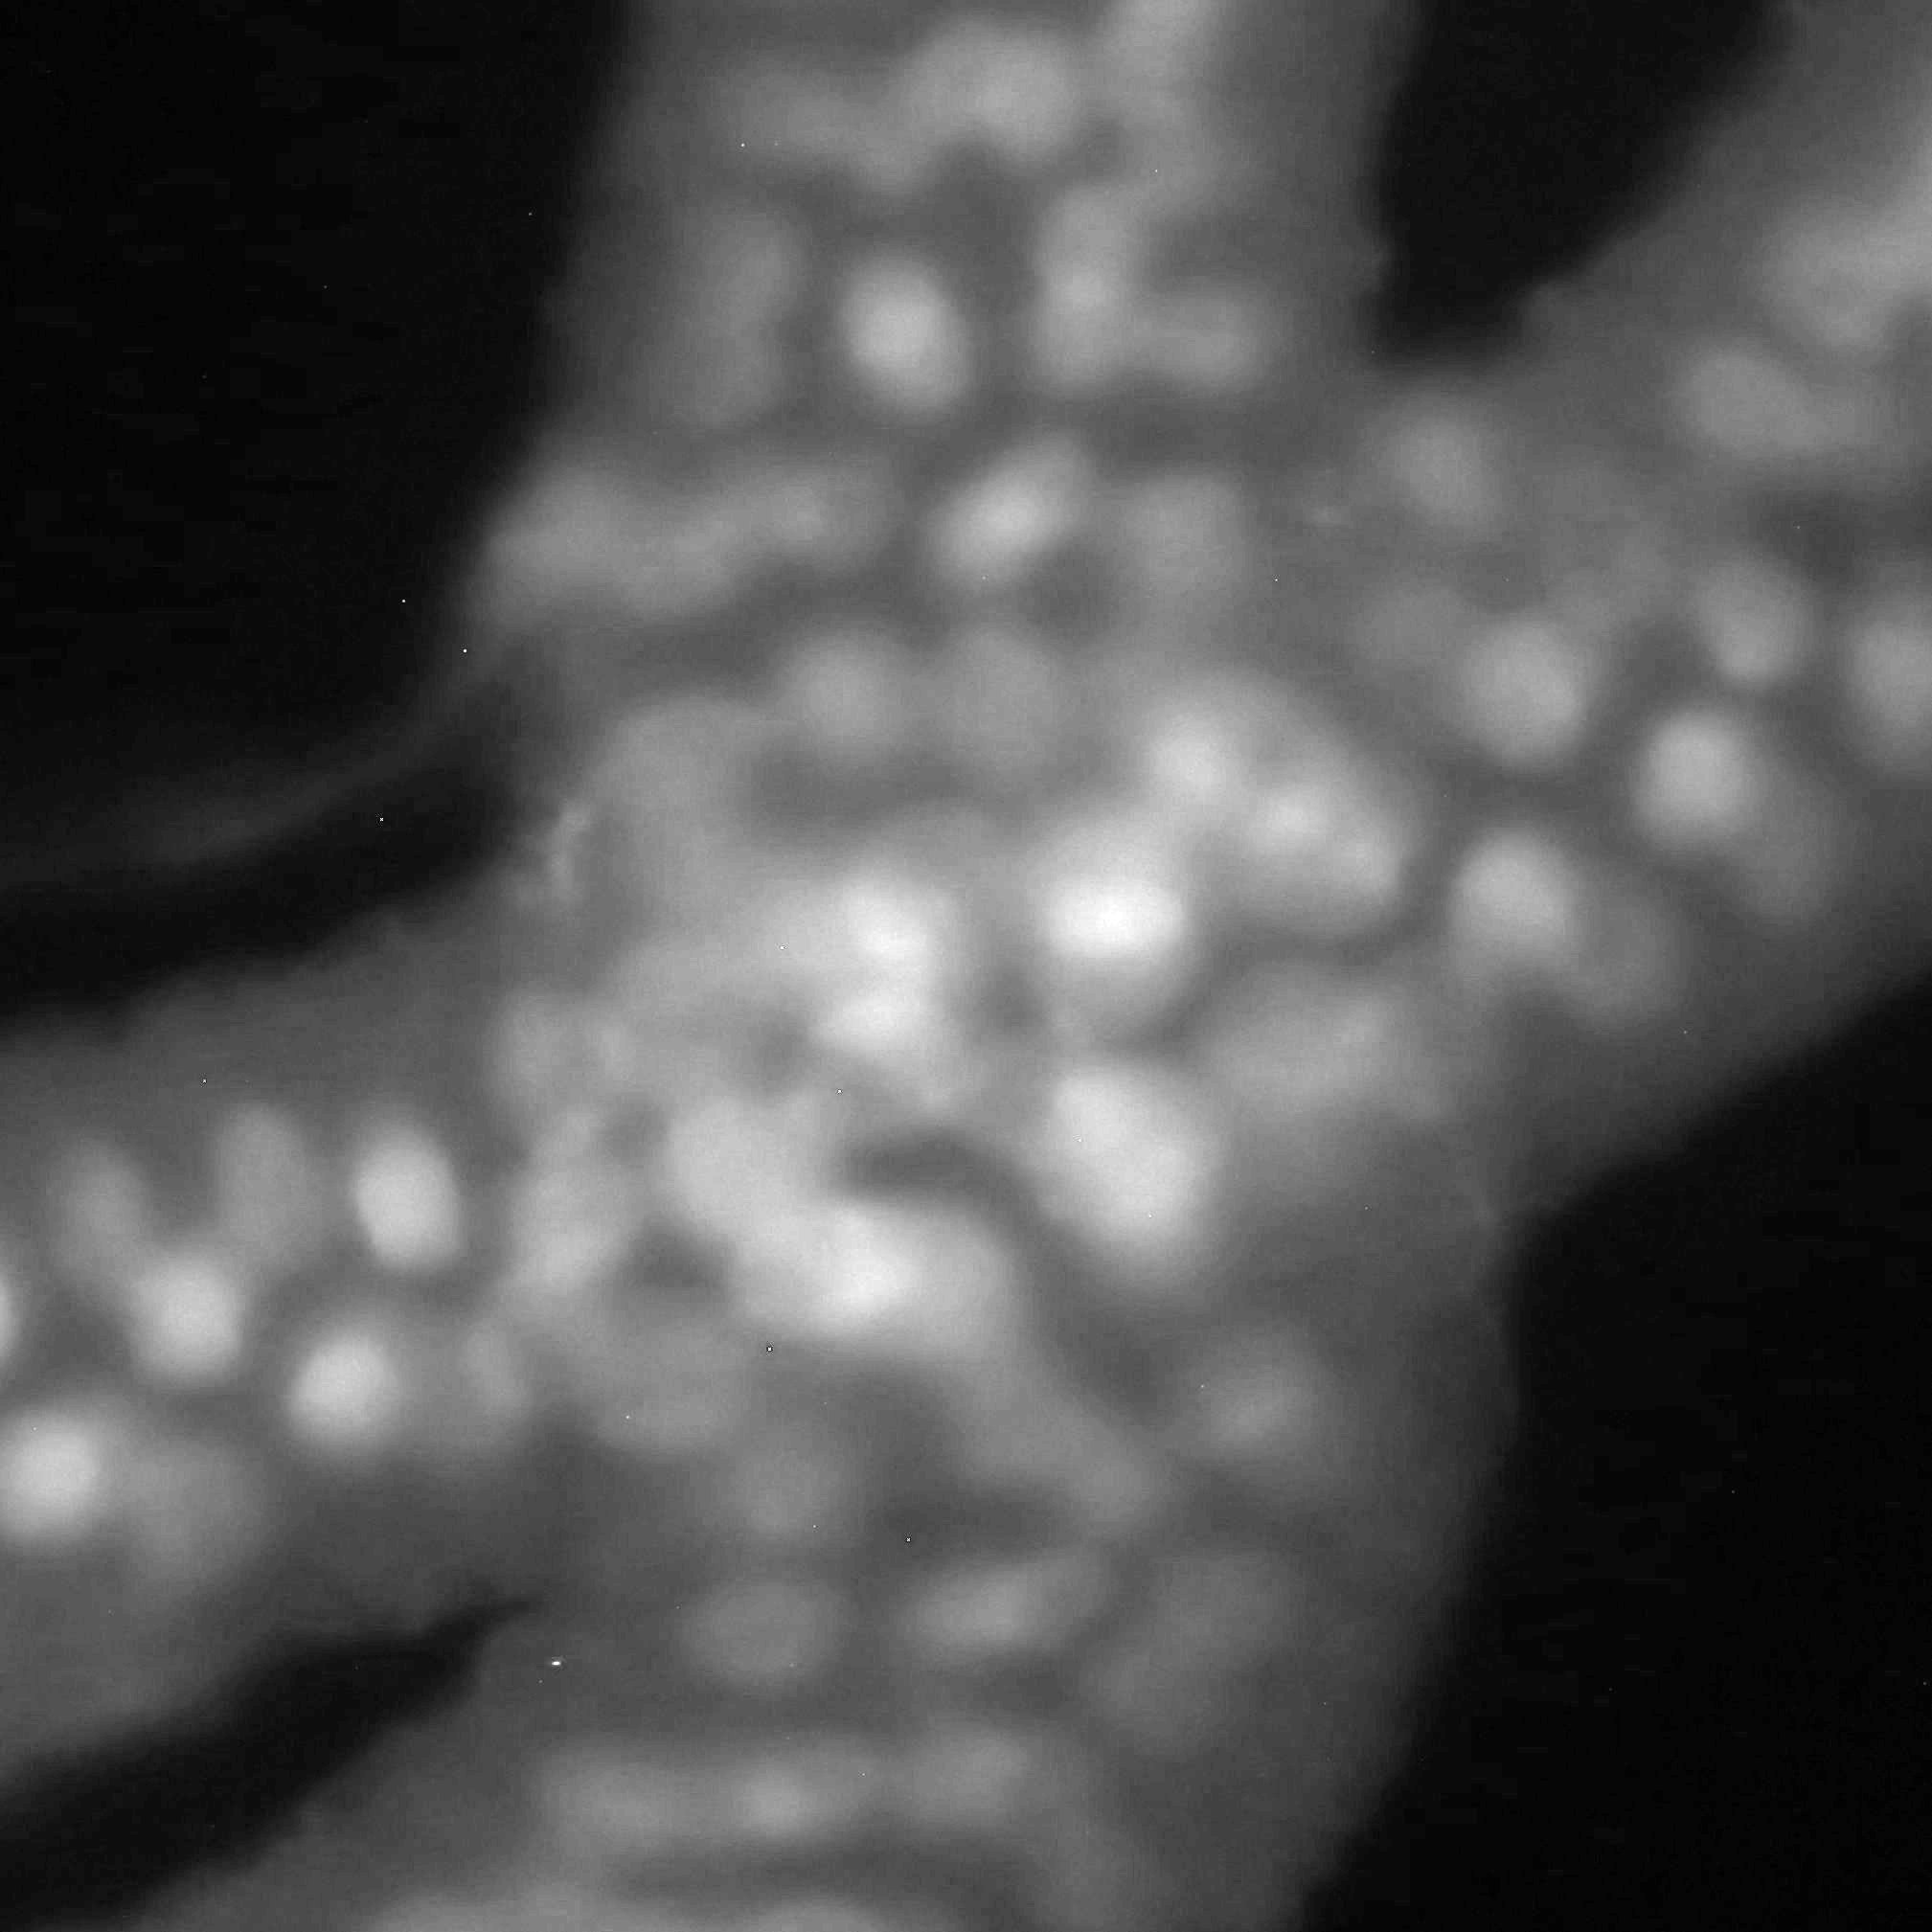
\includegraphics[width=.3\columnwidth]{Exp_2_Microphotography/Figures/33_Blowfly_Fluorescence_01_blue_cropped_32_001norm}}\vspace{-0.7em}
\captionsetup[subfigure]{position=bottom}
\subfloat[Brightfield\label{bsbright}]{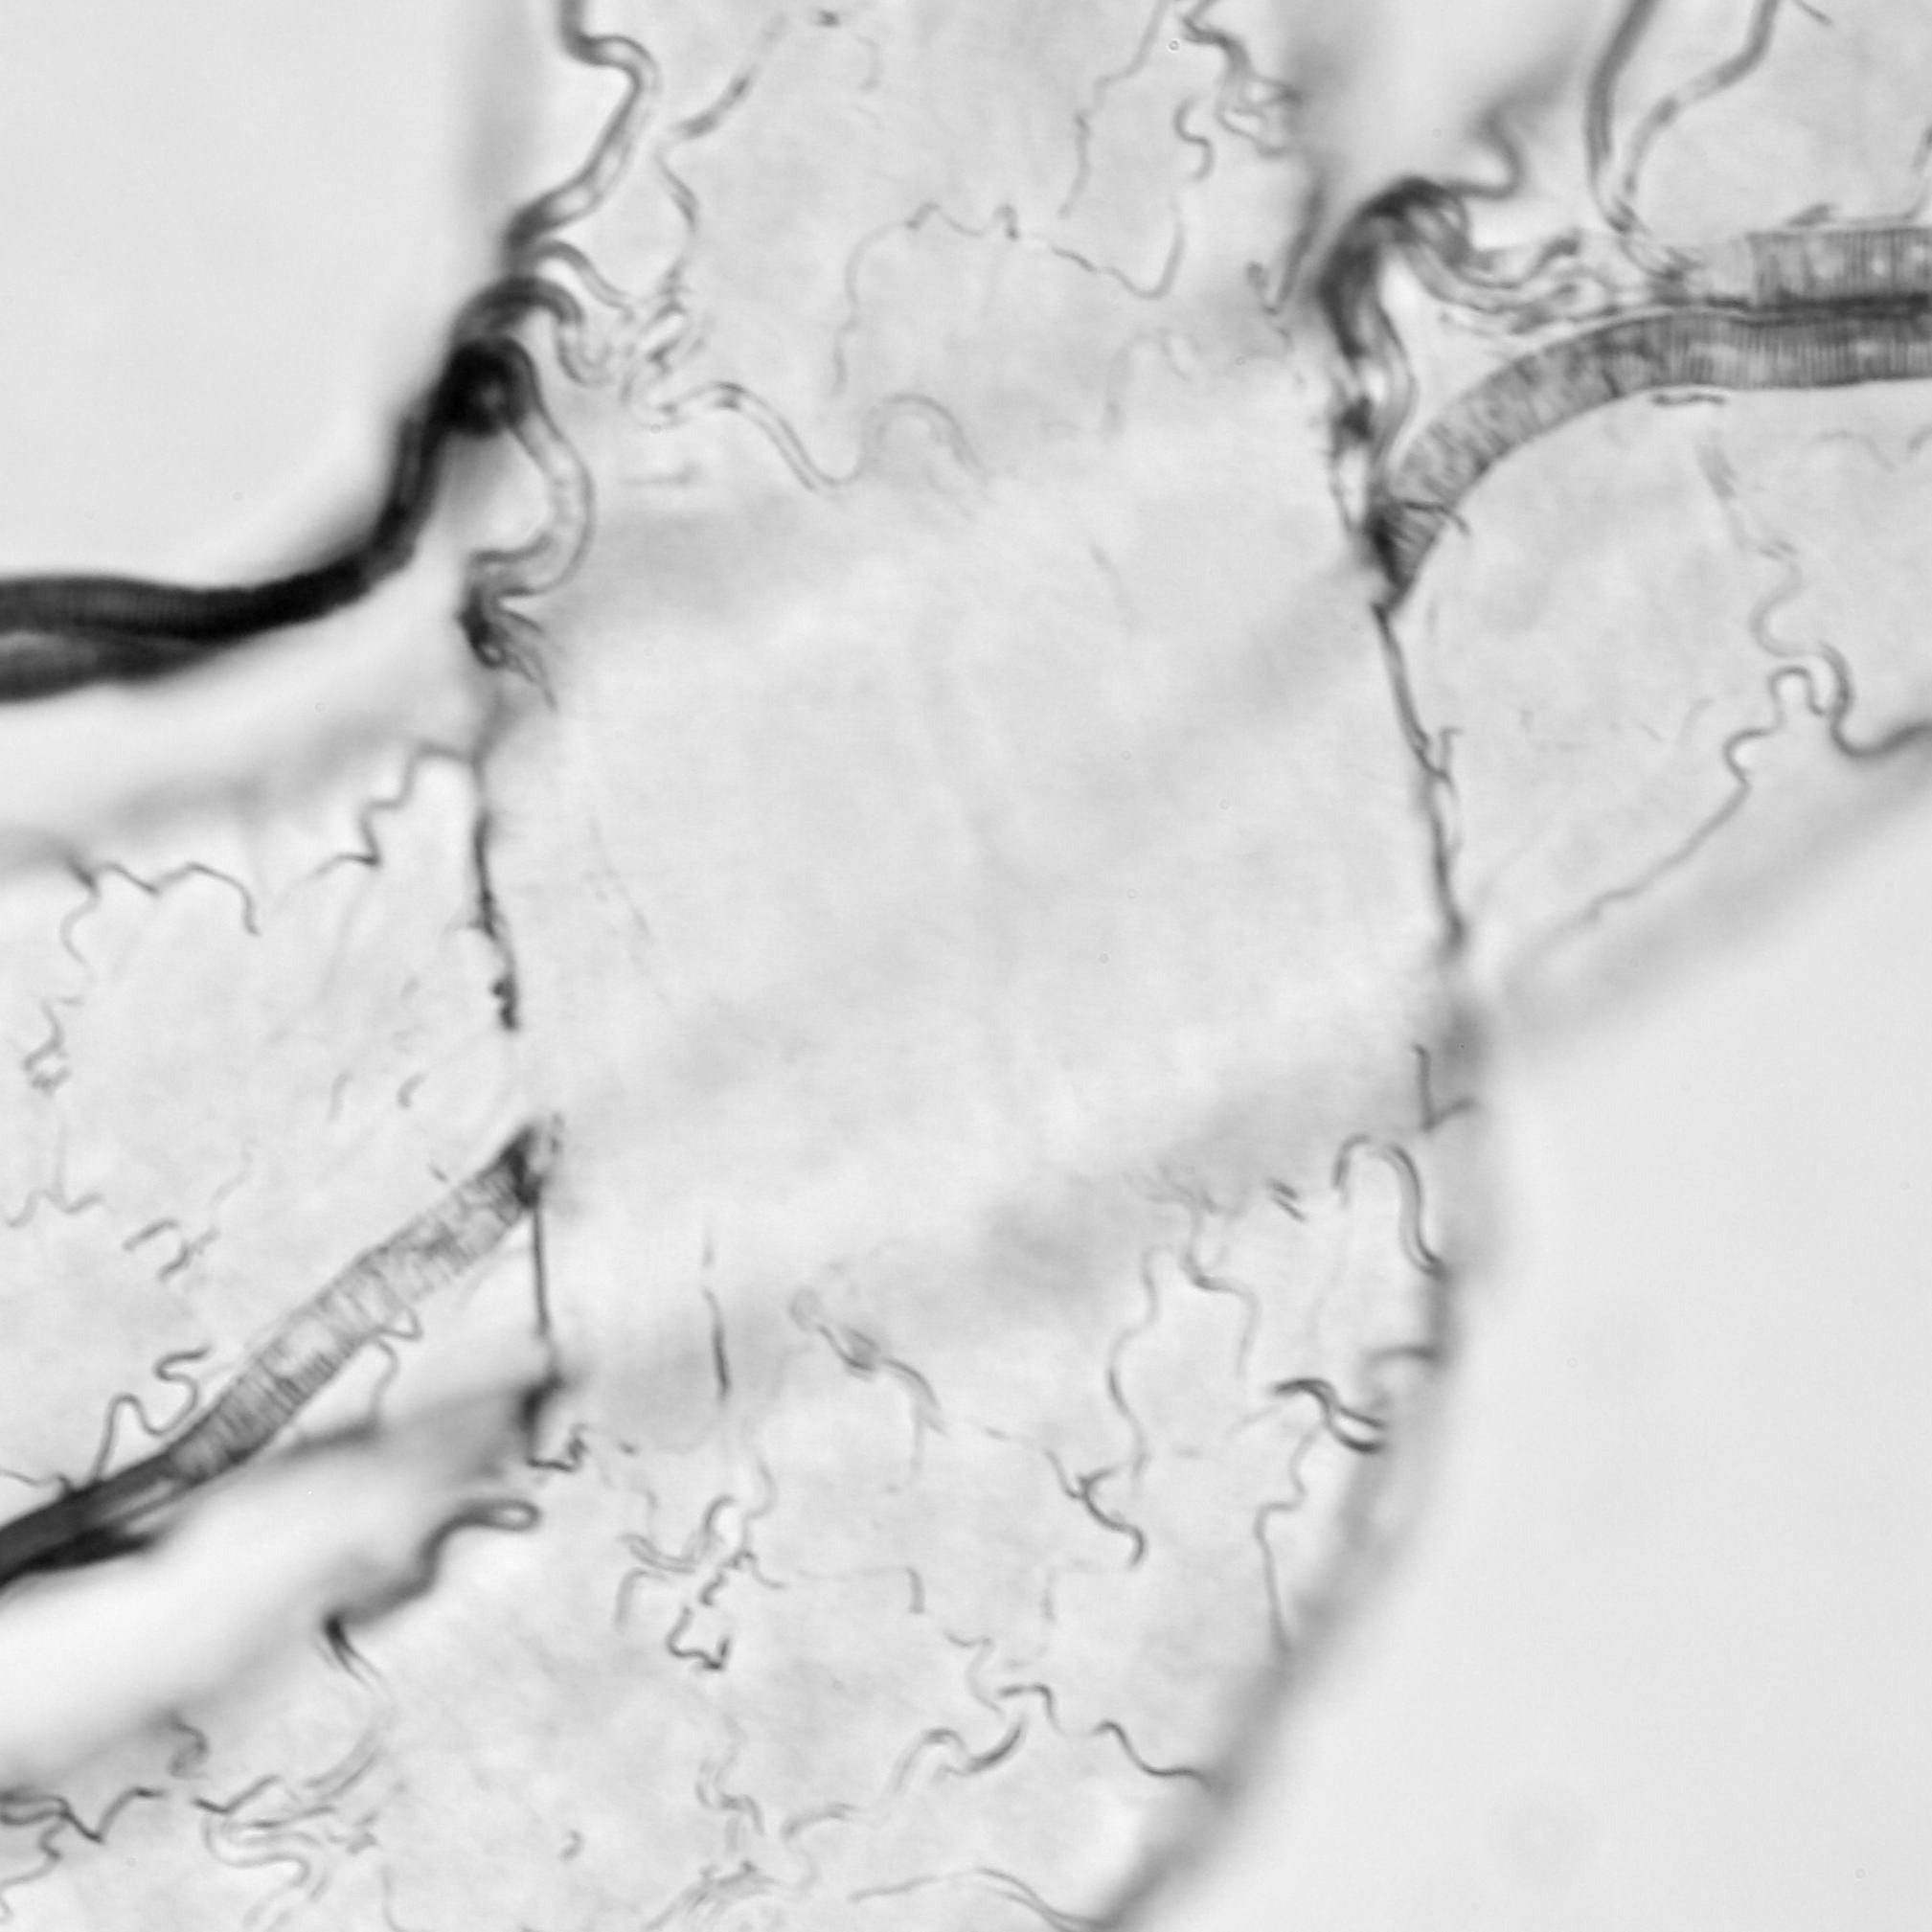
\includegraphics[width=.3\columnwidth]{Exp_2_Microphotography/Figures/19_Blowfly_brightfield_02-1_cropped_32_000norm}} \hspace{0.1mm}
\subfloat[DIC\label{bsdic}]{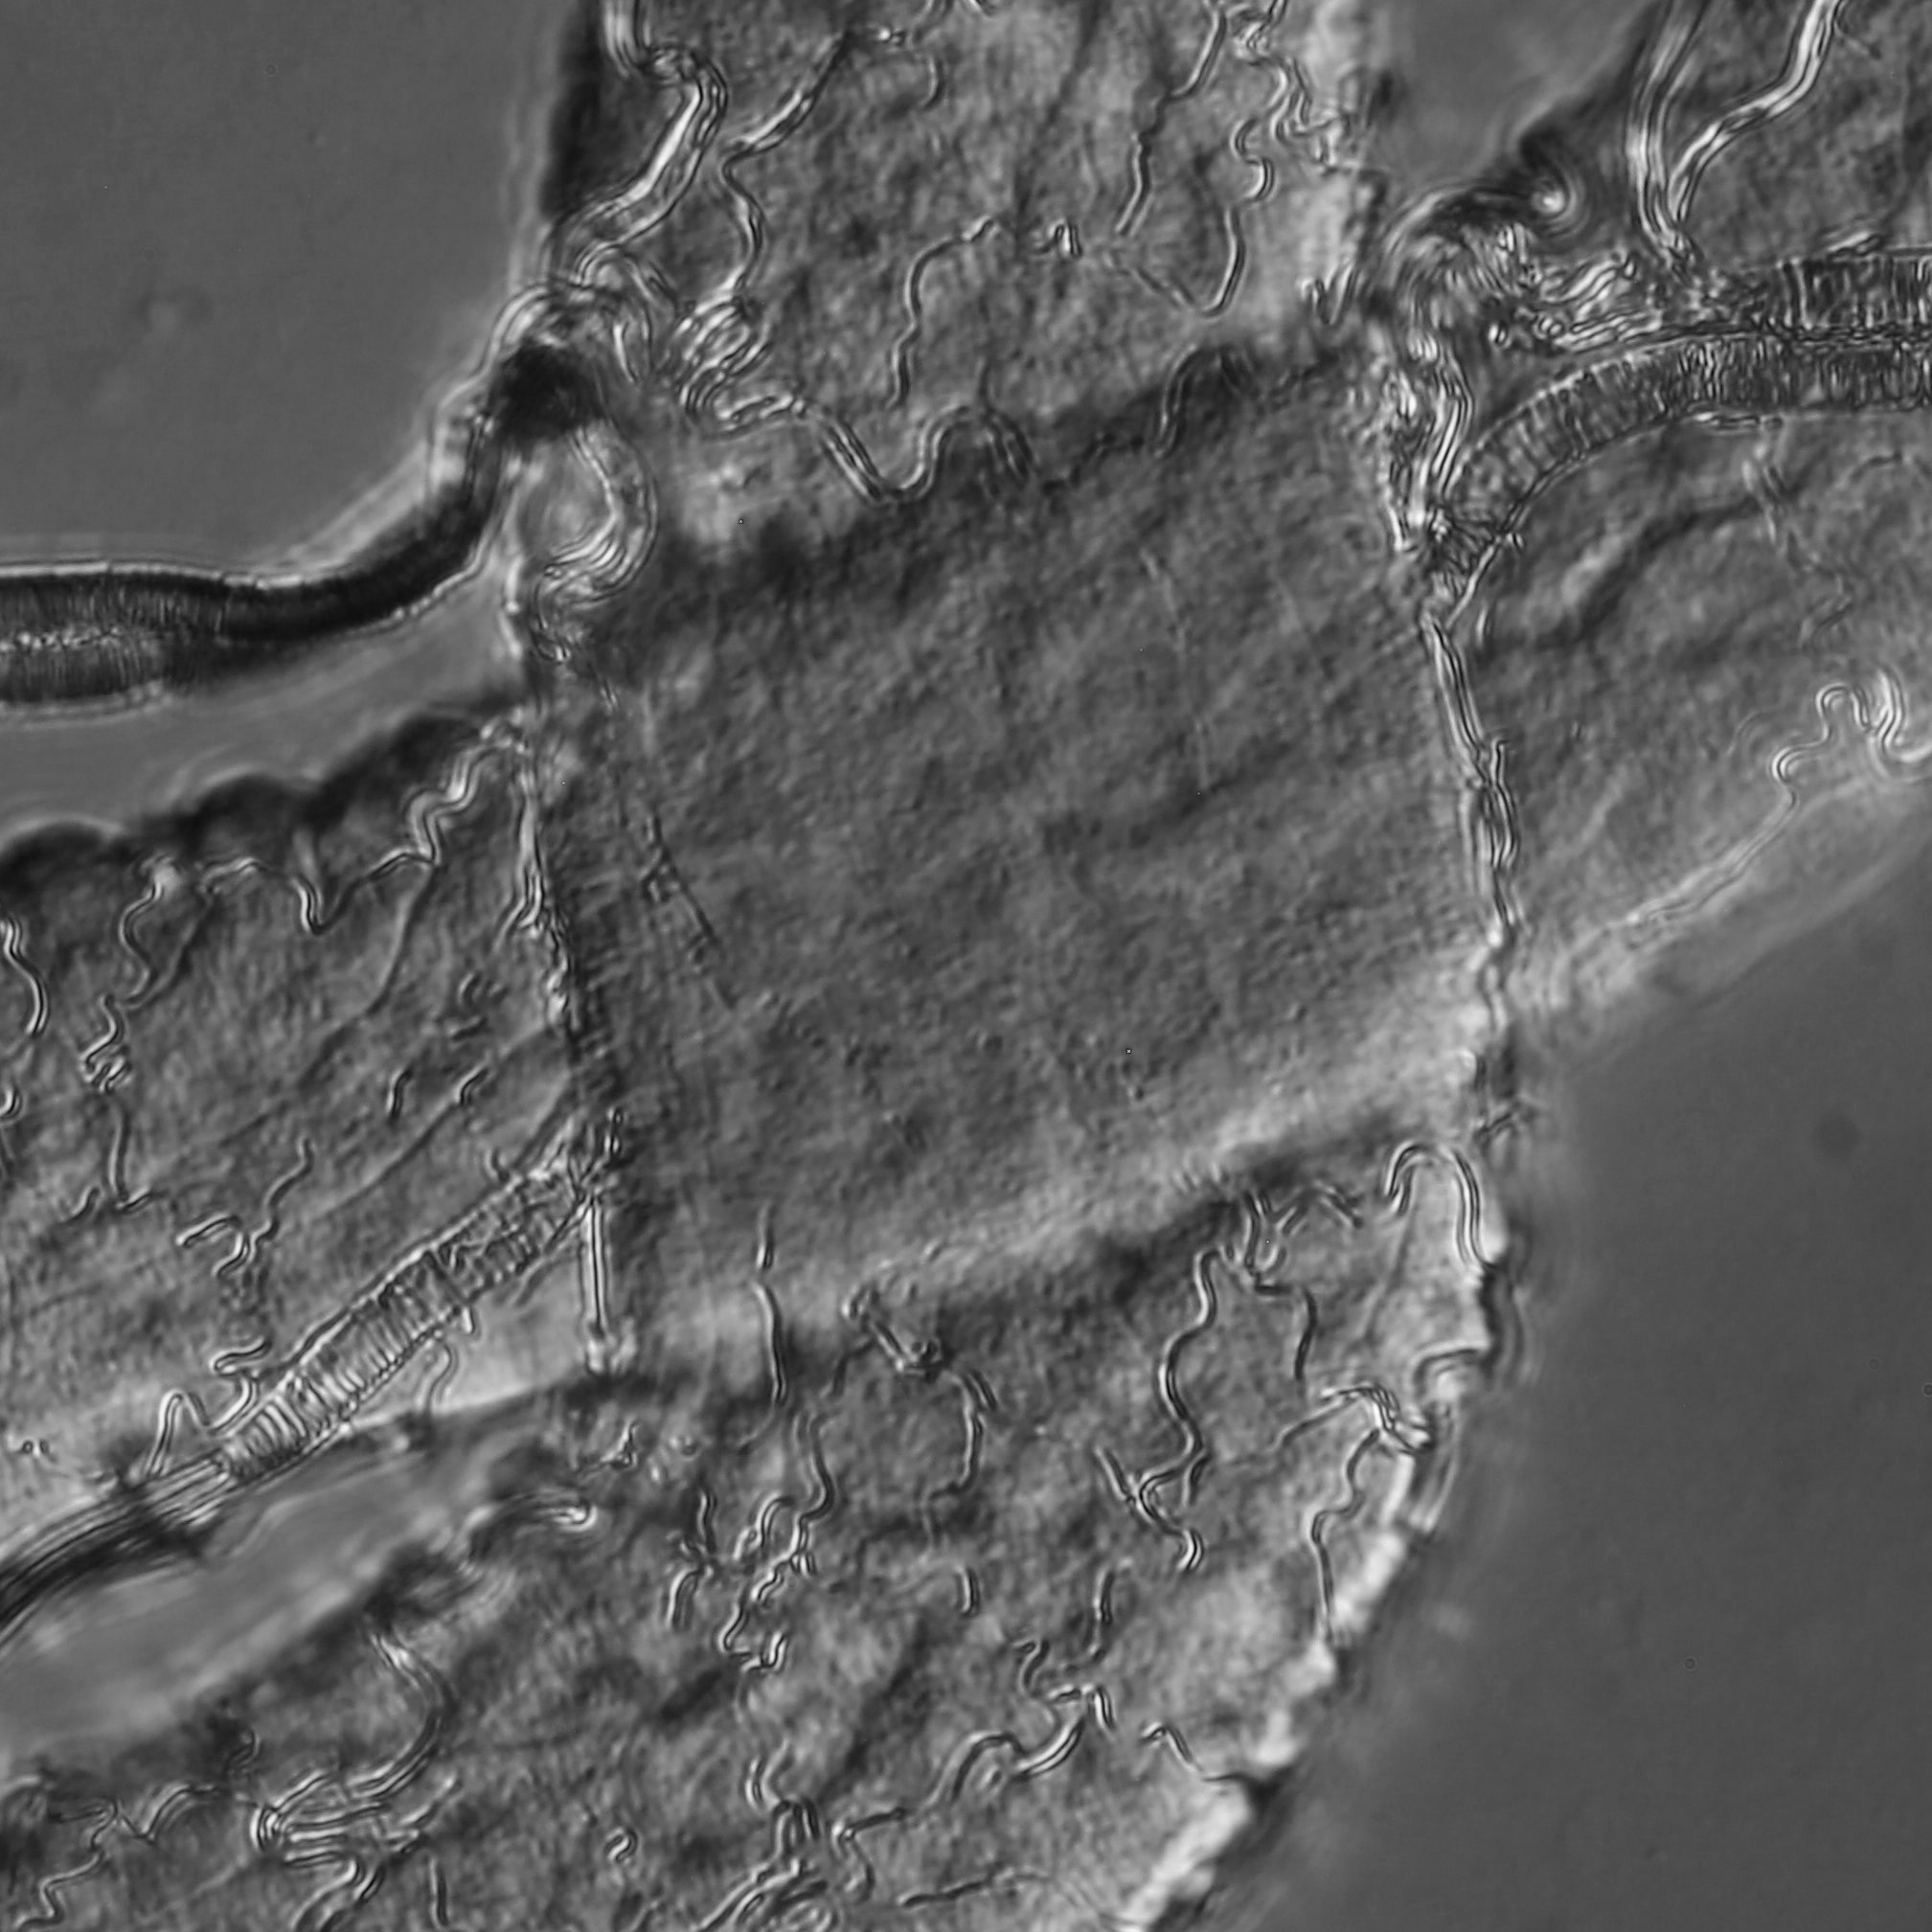
\includegraphics[width=.3\columnwidth]{Exp_2_Microphotography/Figures/Blowfly_DIC_02-1_cropped_32_000norm}} \hspace{0.1mm}
\subfloat[Phase Contrast\label{bsphase}]{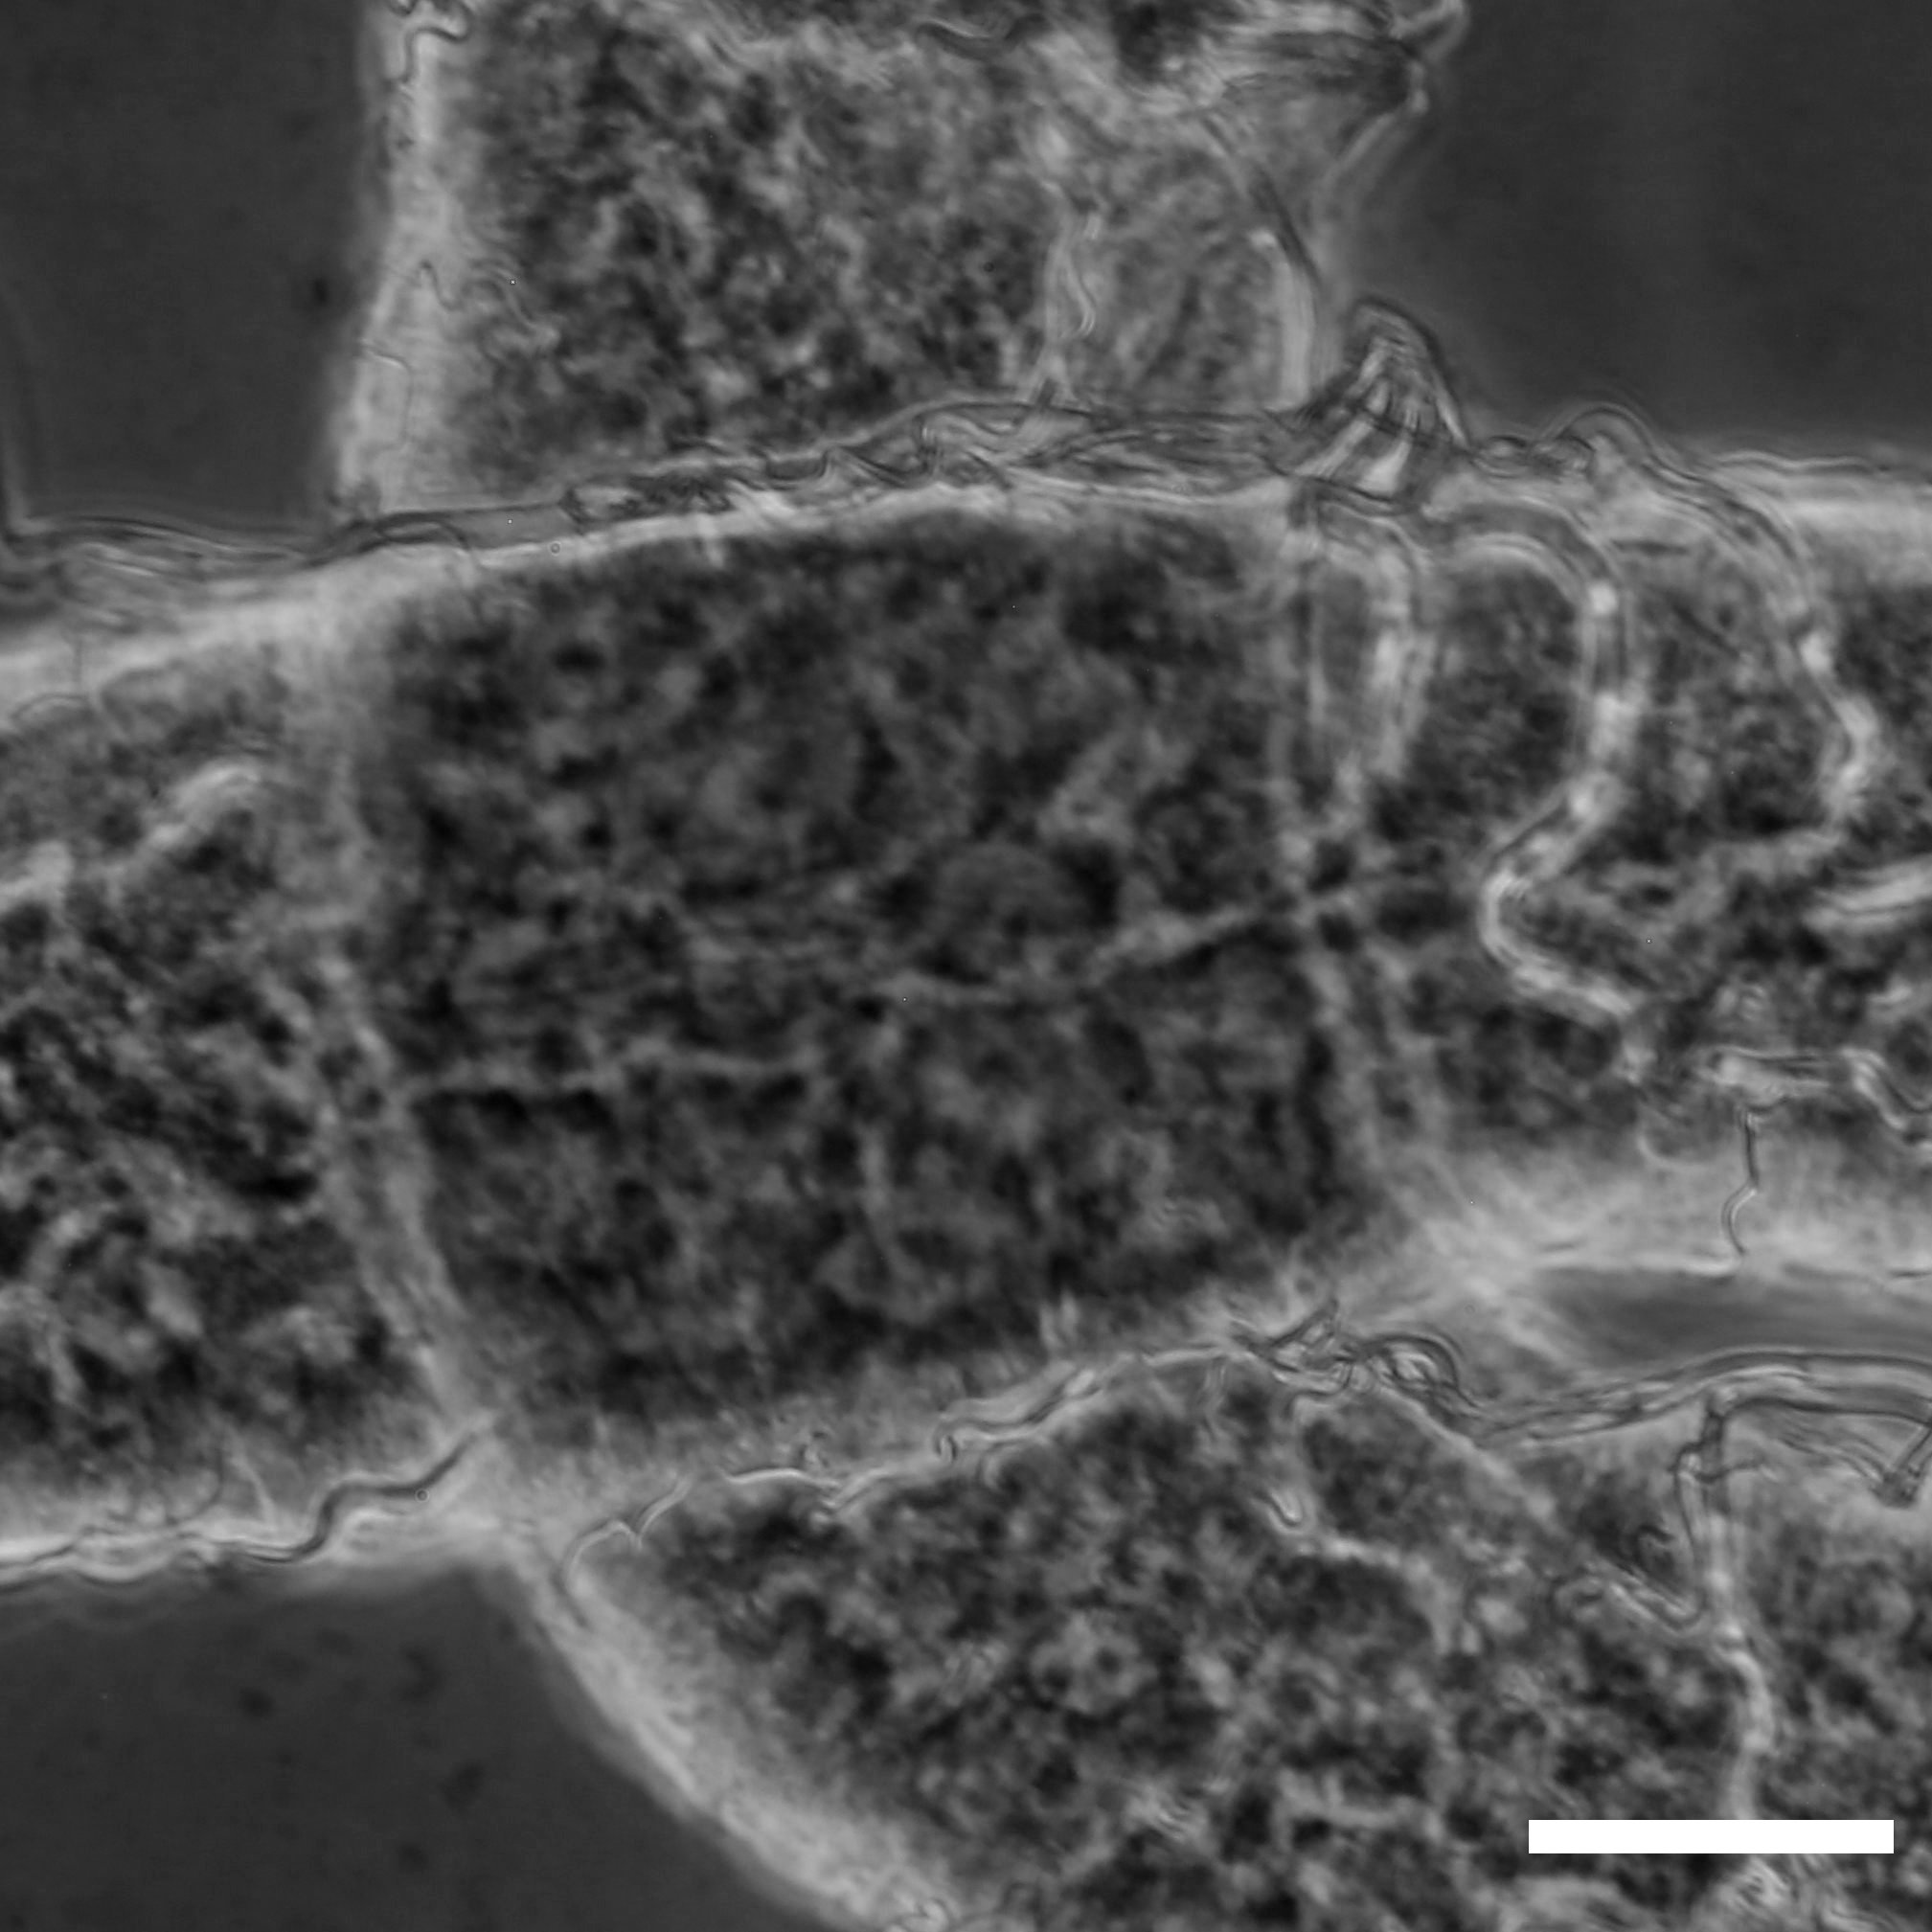
\includegraphics[width=.3\columnwidth]{Exp_2_Microphotography/Figures/22 Blowfly_phasecontrast_02-1_cropped_32_000norm_scale25}}
\caption{Blowfly under fluorescence, brightfield, DIC, and phase contrast microscopy. 
Septate junctions labelled by immunofluorescene (AlexaFluor568), actin by AlexaFluor488-Phalloidin, and the nucleus by DAPI. 
Objective lens: Plan Neofluar 40$\times$/0.75 Ph2. 
Scalebar is 25 $\mu$m.} 
\label{fig:blow}
\end{figure}

The blowfly salivary gland specimen was labelled using three different fluorescent markers, namely; DAPI, AlexaFluor488-Phalloidin, and immunofluorescence against FasIII. 
Each of the label binds to certain part of the salivary gland. 
These fluorescent labels can be excited by light with the corresponding excitation wavelength. 
Immunofluorescence of Fasciclin III on the septate junctions of the cell utilizes green excitation and produces red emission (Fig.~\ref{bsred}). 
The green emission of AlexaFluor488-Phalloidin (Fig.~\ref{bsgreen}) is excited by blue excitation light, and shows the actin filaments of the cell. 
The round structures in Fig.~\ref{bsblue} shows the nucleus of the cell, in which DAPI binds to DNA and emits blue emission. 
All these organelles would otherwise be hardly visible in the brightfield microscopy (Fig.~\ref{bsbright}). 
DIC and phase contrast microscopy (Fig.~\ref{bsdic} \&~\ref{bsphase} respectively) provide a more detailed look into the specimen and reveal structures which in brightfield microscopy can only be hazily visible.

%--------------------------------------------------
\subsection{Pinewood and Starch}

\begin{figure}[ht]
\centering
\captionsetup[subfigure]{position=top}
\subfloat[Brightfield\label{pbright}]{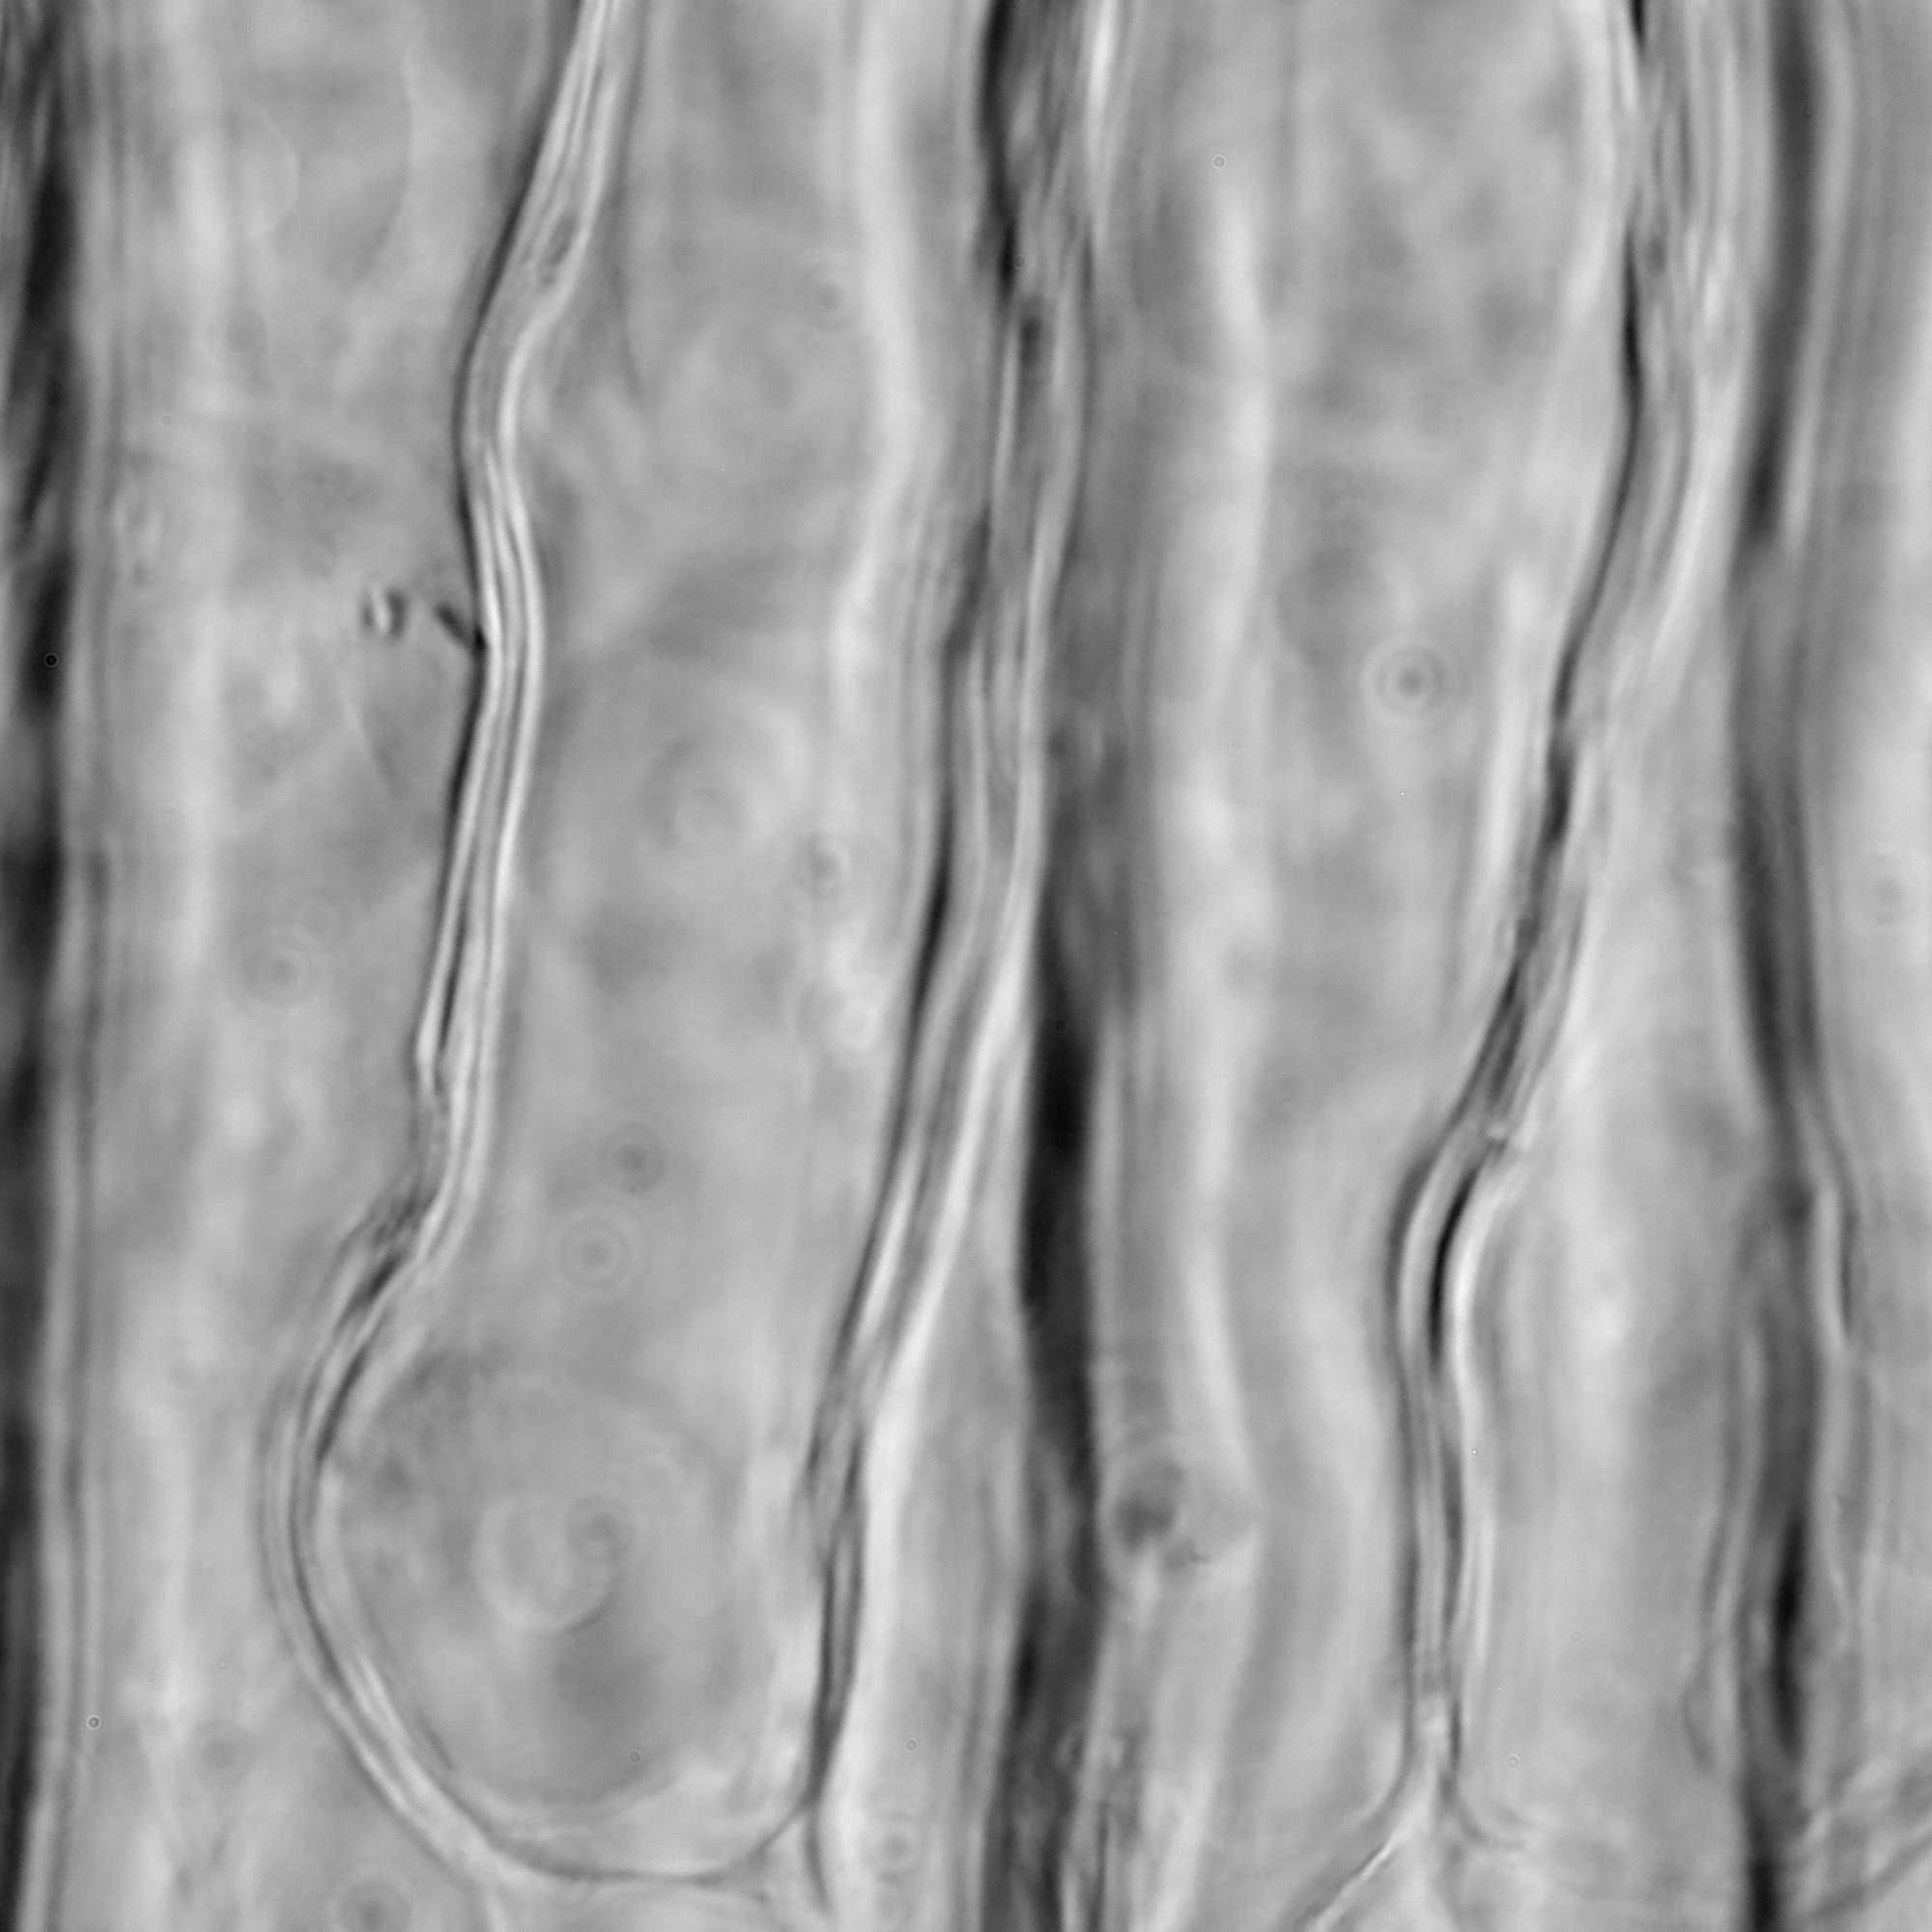
\includegraphics[width=.3\columnwidth]{Exp_2_Microphotography/Figures/38_Pinewood_Brightfield_01_straight_cropped_32_000norm}} \hspace{0.1mm}
\subfloat[DIC\label{pdic}]{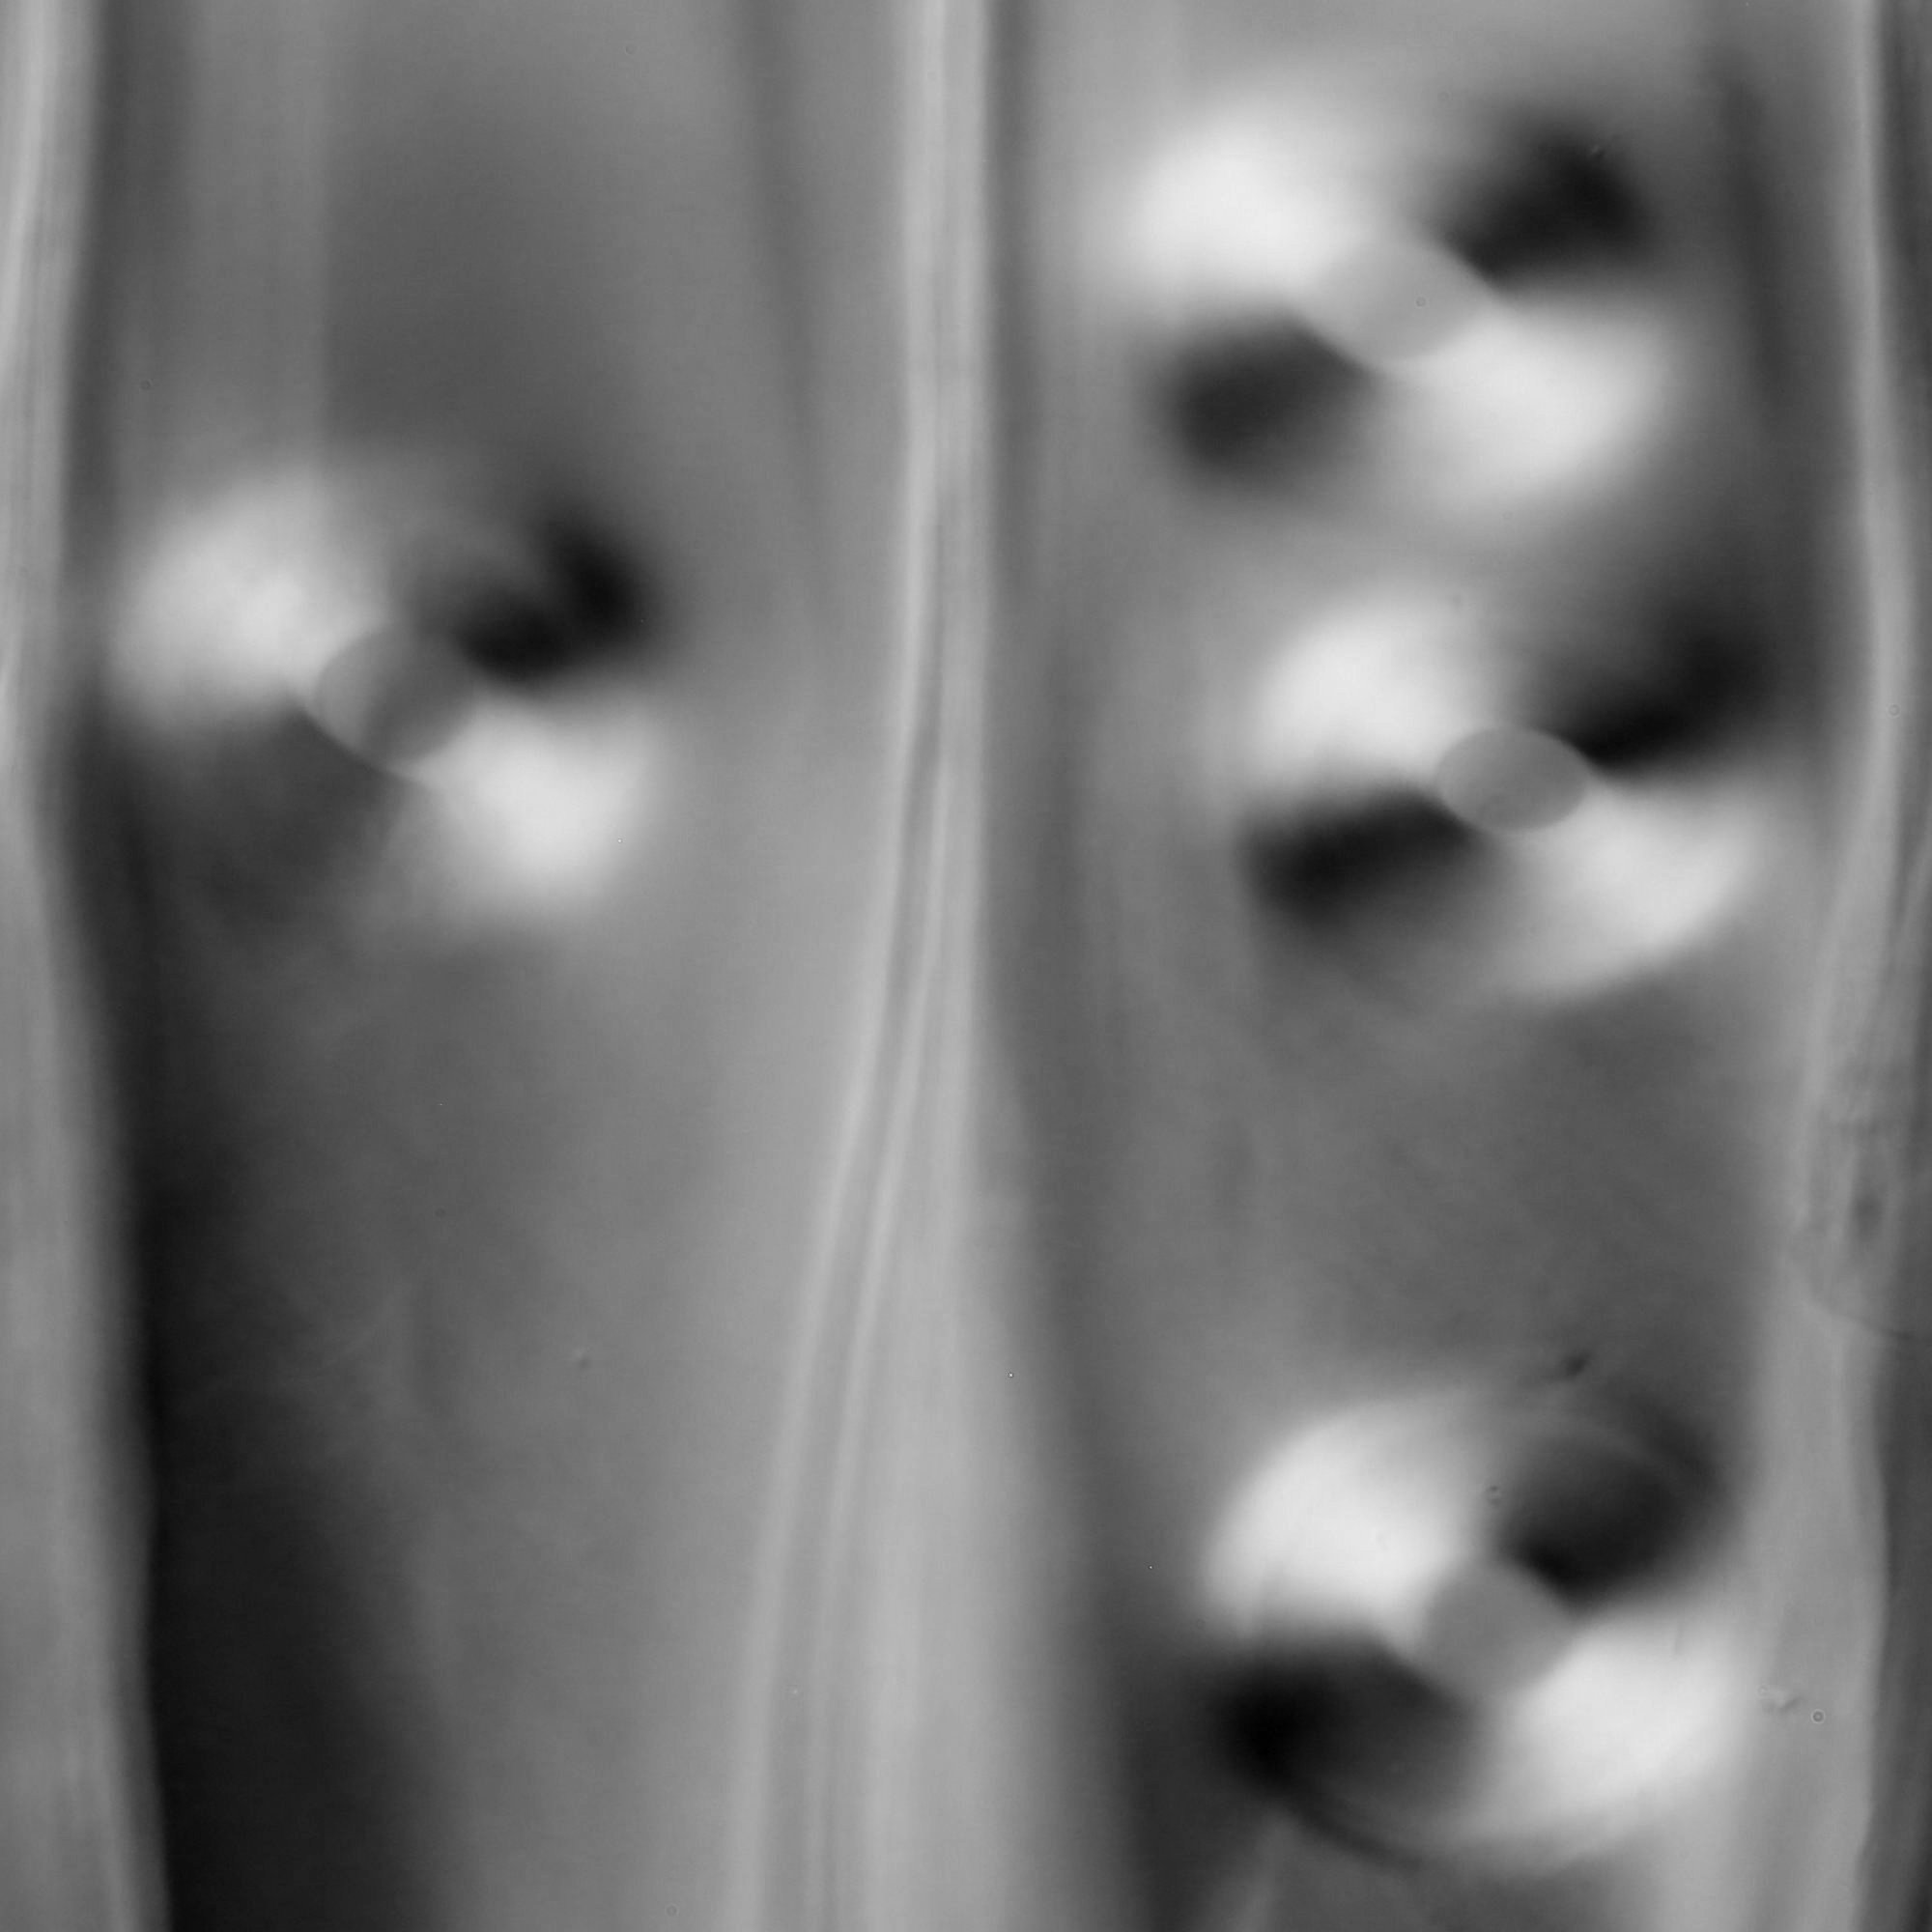
\includegraphics[width=.3\columnwidth]{Exp_2_Microphotography/Figures/40_Pinewood_DIC_02_cropped_32_000norm}}\hspace{0.1mm}
\subfloat[Polarization\label{ppol}]{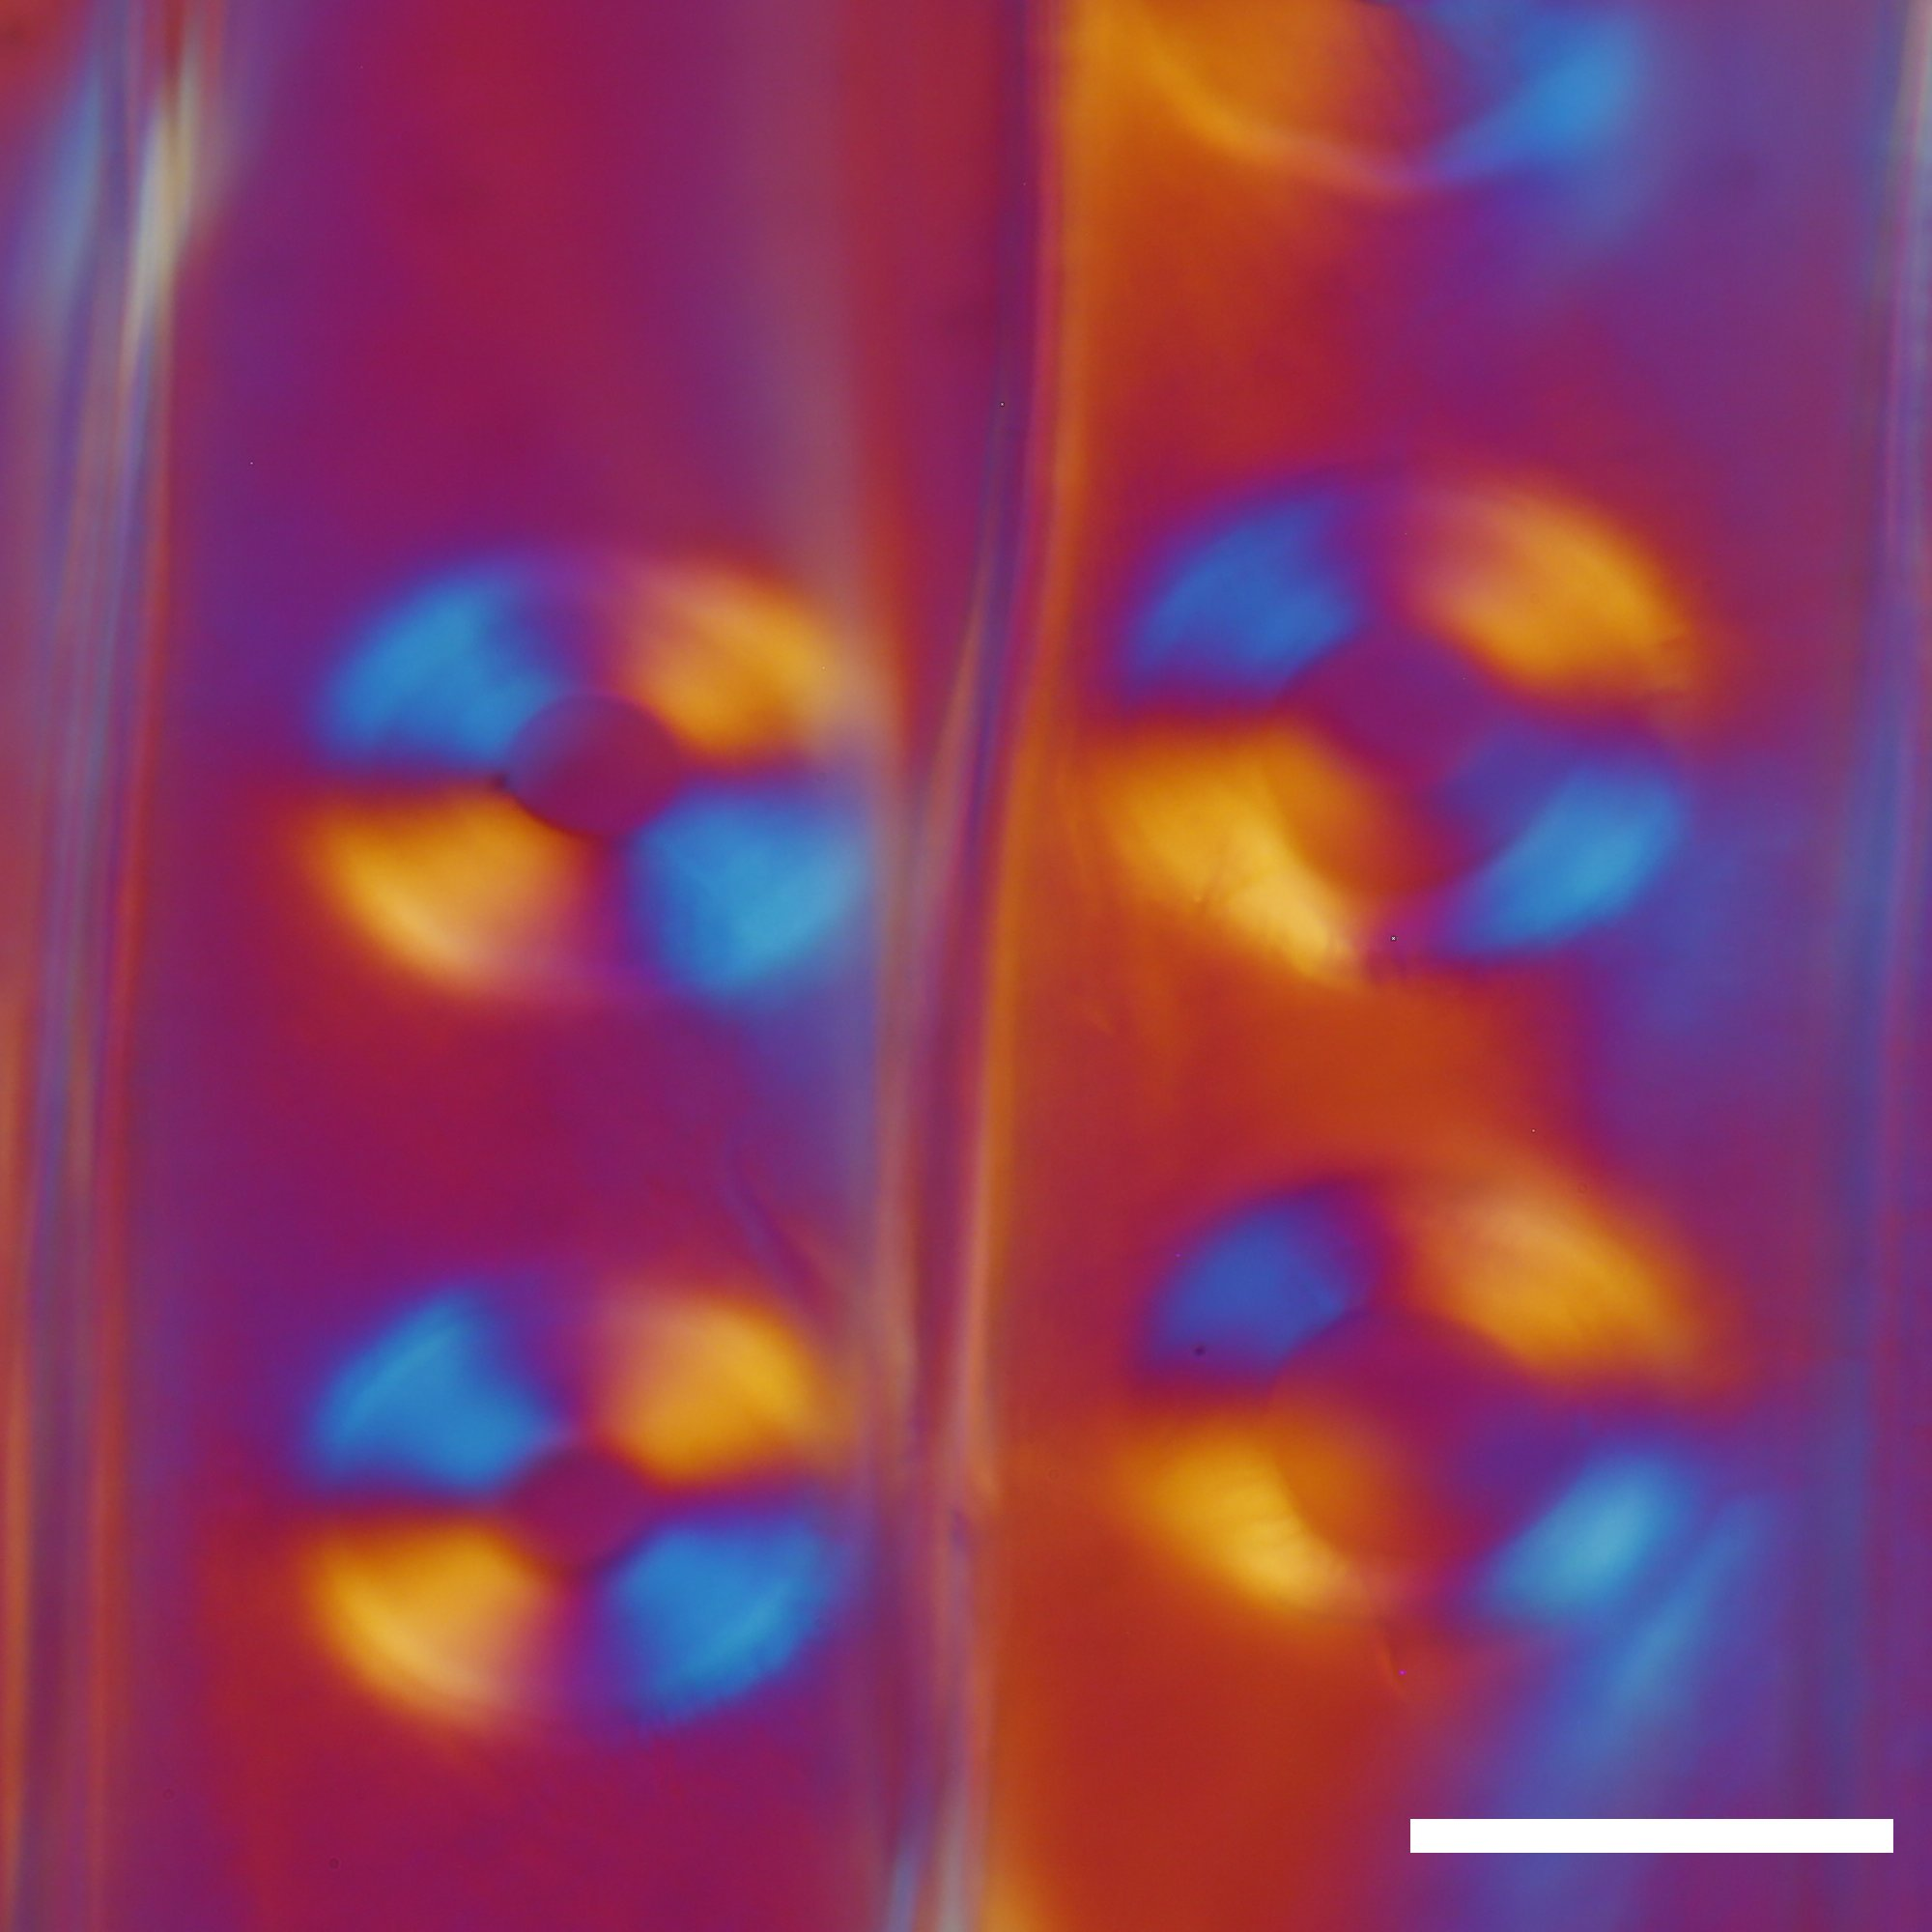
\includegraphics[width=.3\columnwidth]{Exp_2_Microphotography/Figures/42_Pinewood_Polarization_02_cropped_scale20}}\vspace{-0.7em}
\captionsetup[subfigure]{position=bottom}
\subfloat[Brightfield\label{sbright}]{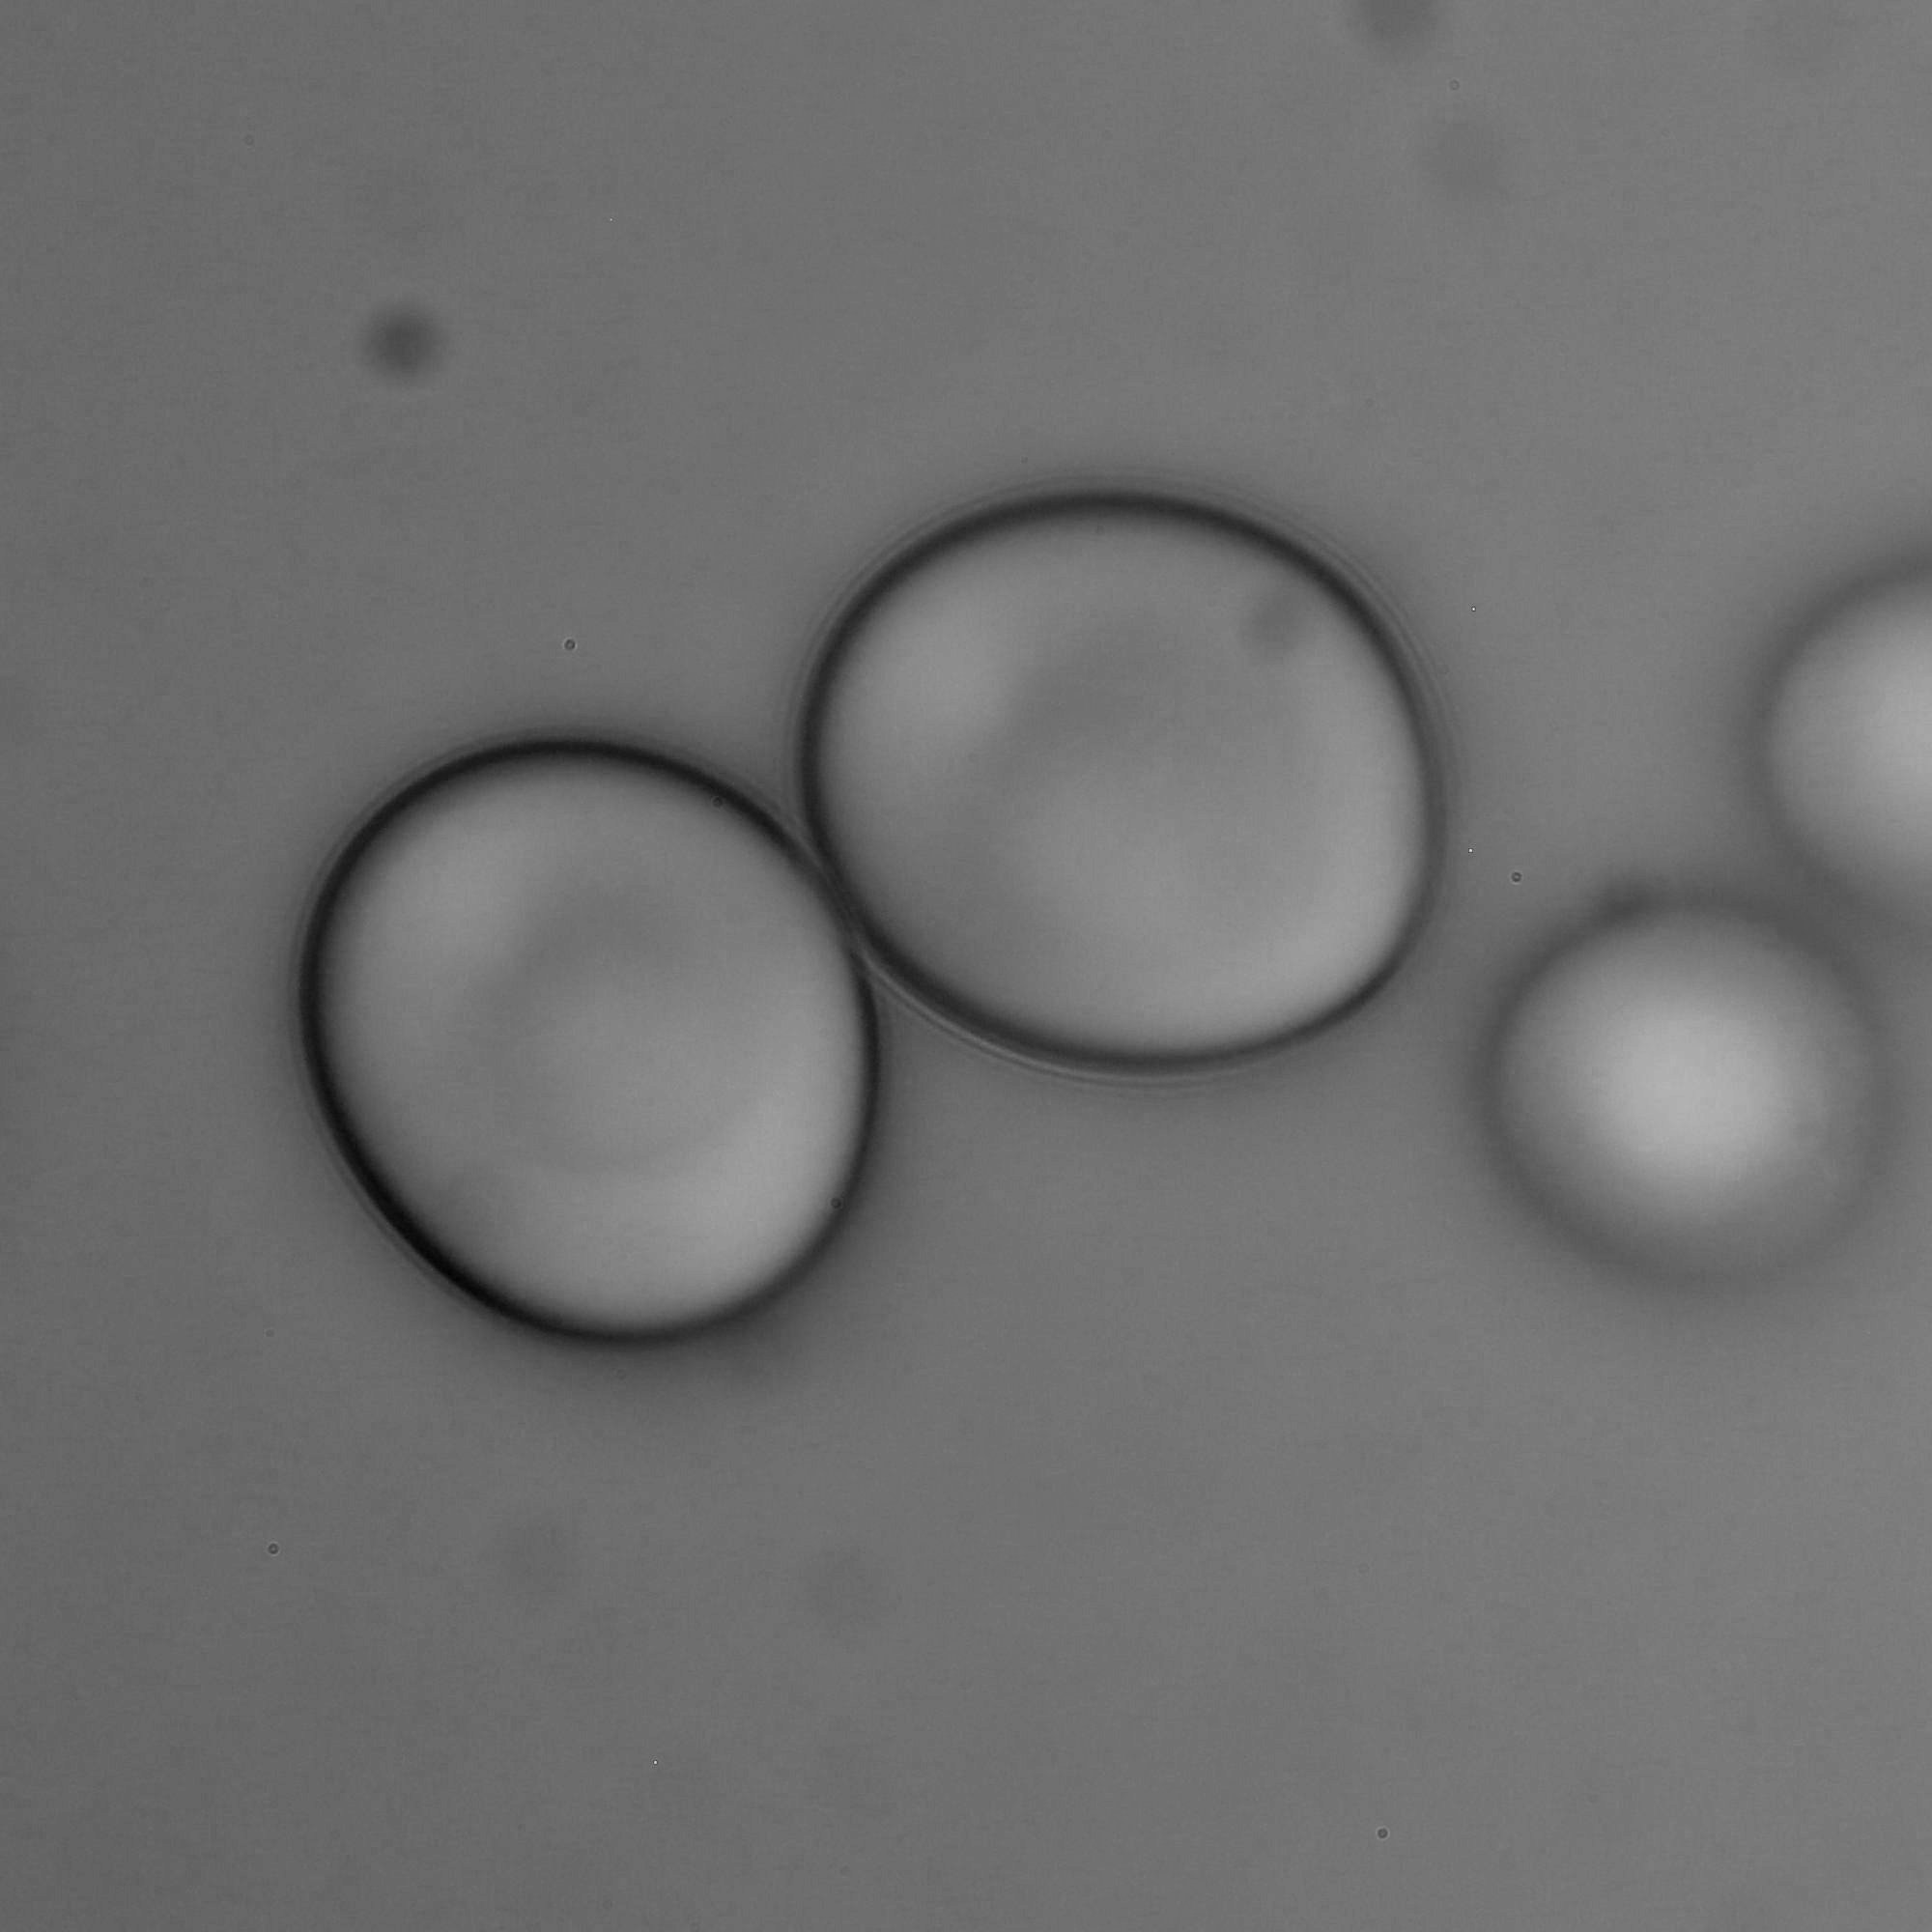
\includegraphics[width=.3\columnwidth]{Exp_2_Microphotography/Figures/53_Starch_brightfield_03_cropped_32_000norm}} \hspace{0.1mm}
\subfloat[DIC\label{sdic}]{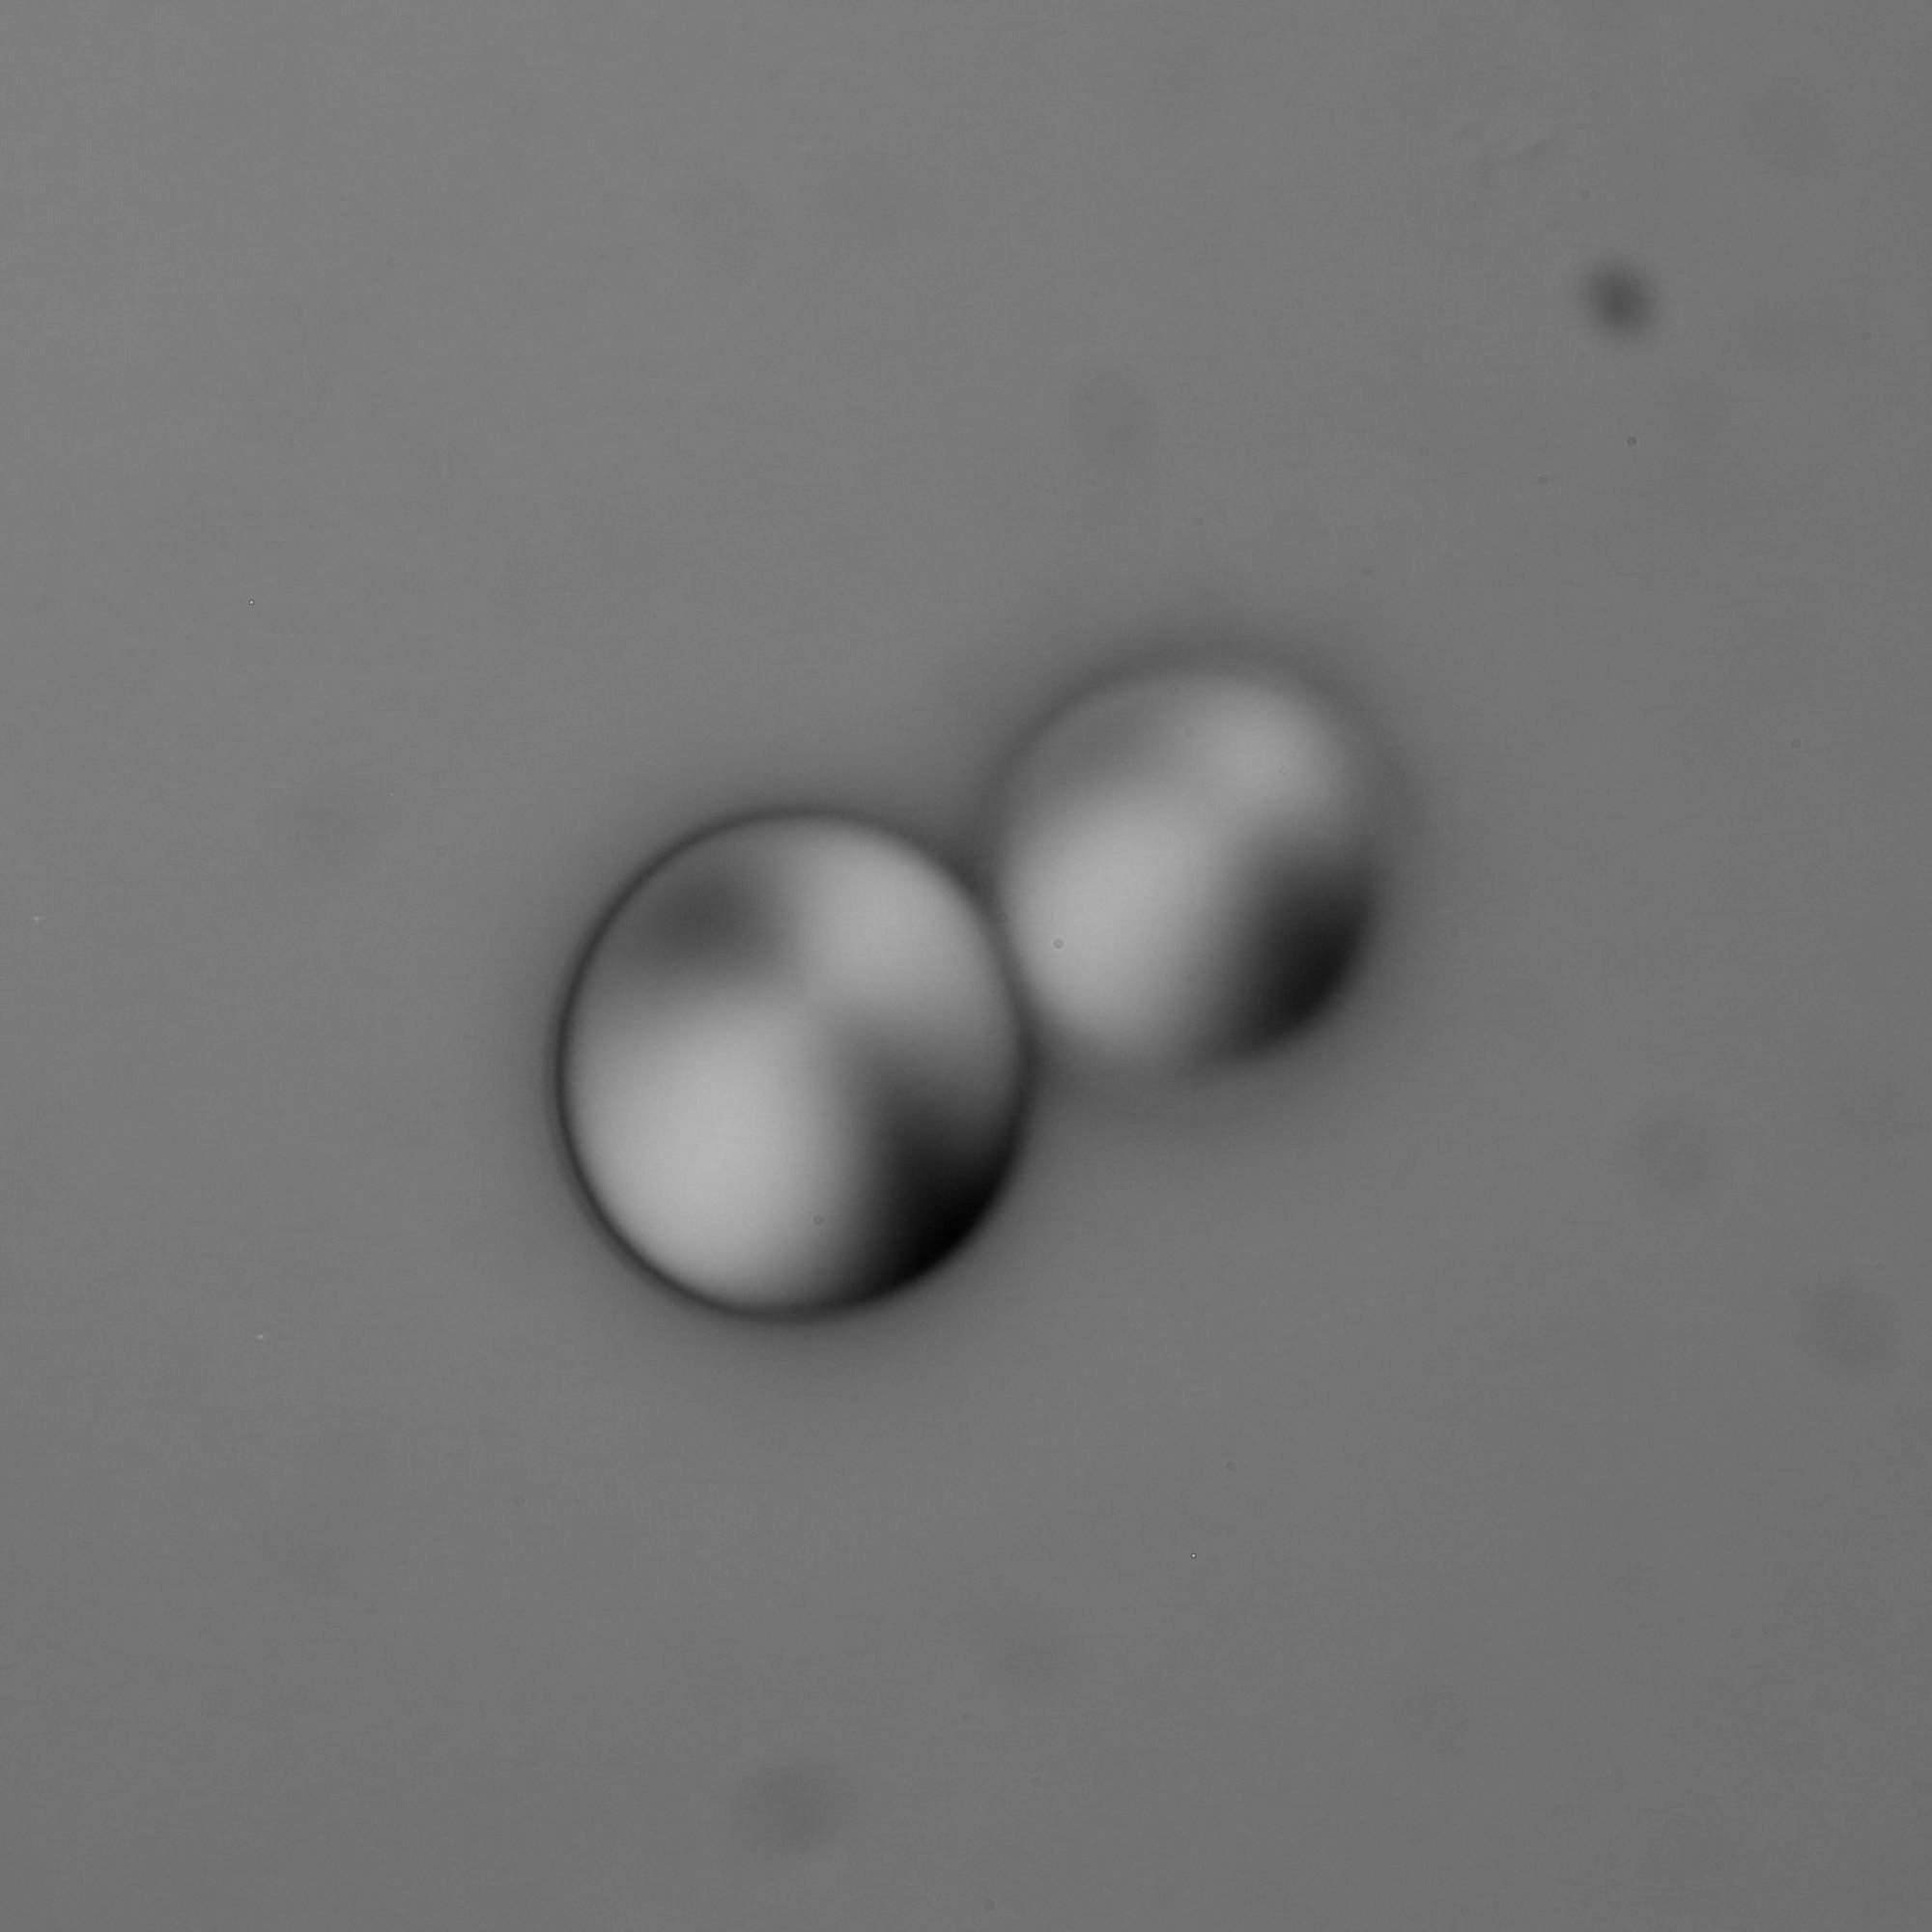
\includegraphics[width=.3\columnwidth]{Exp_2_Microphotography/Figures/50_Starch_DIC_02_cropped_32_000norm}} \hspace{0.1mm}
\subfloat[Polarization\label{spol}]{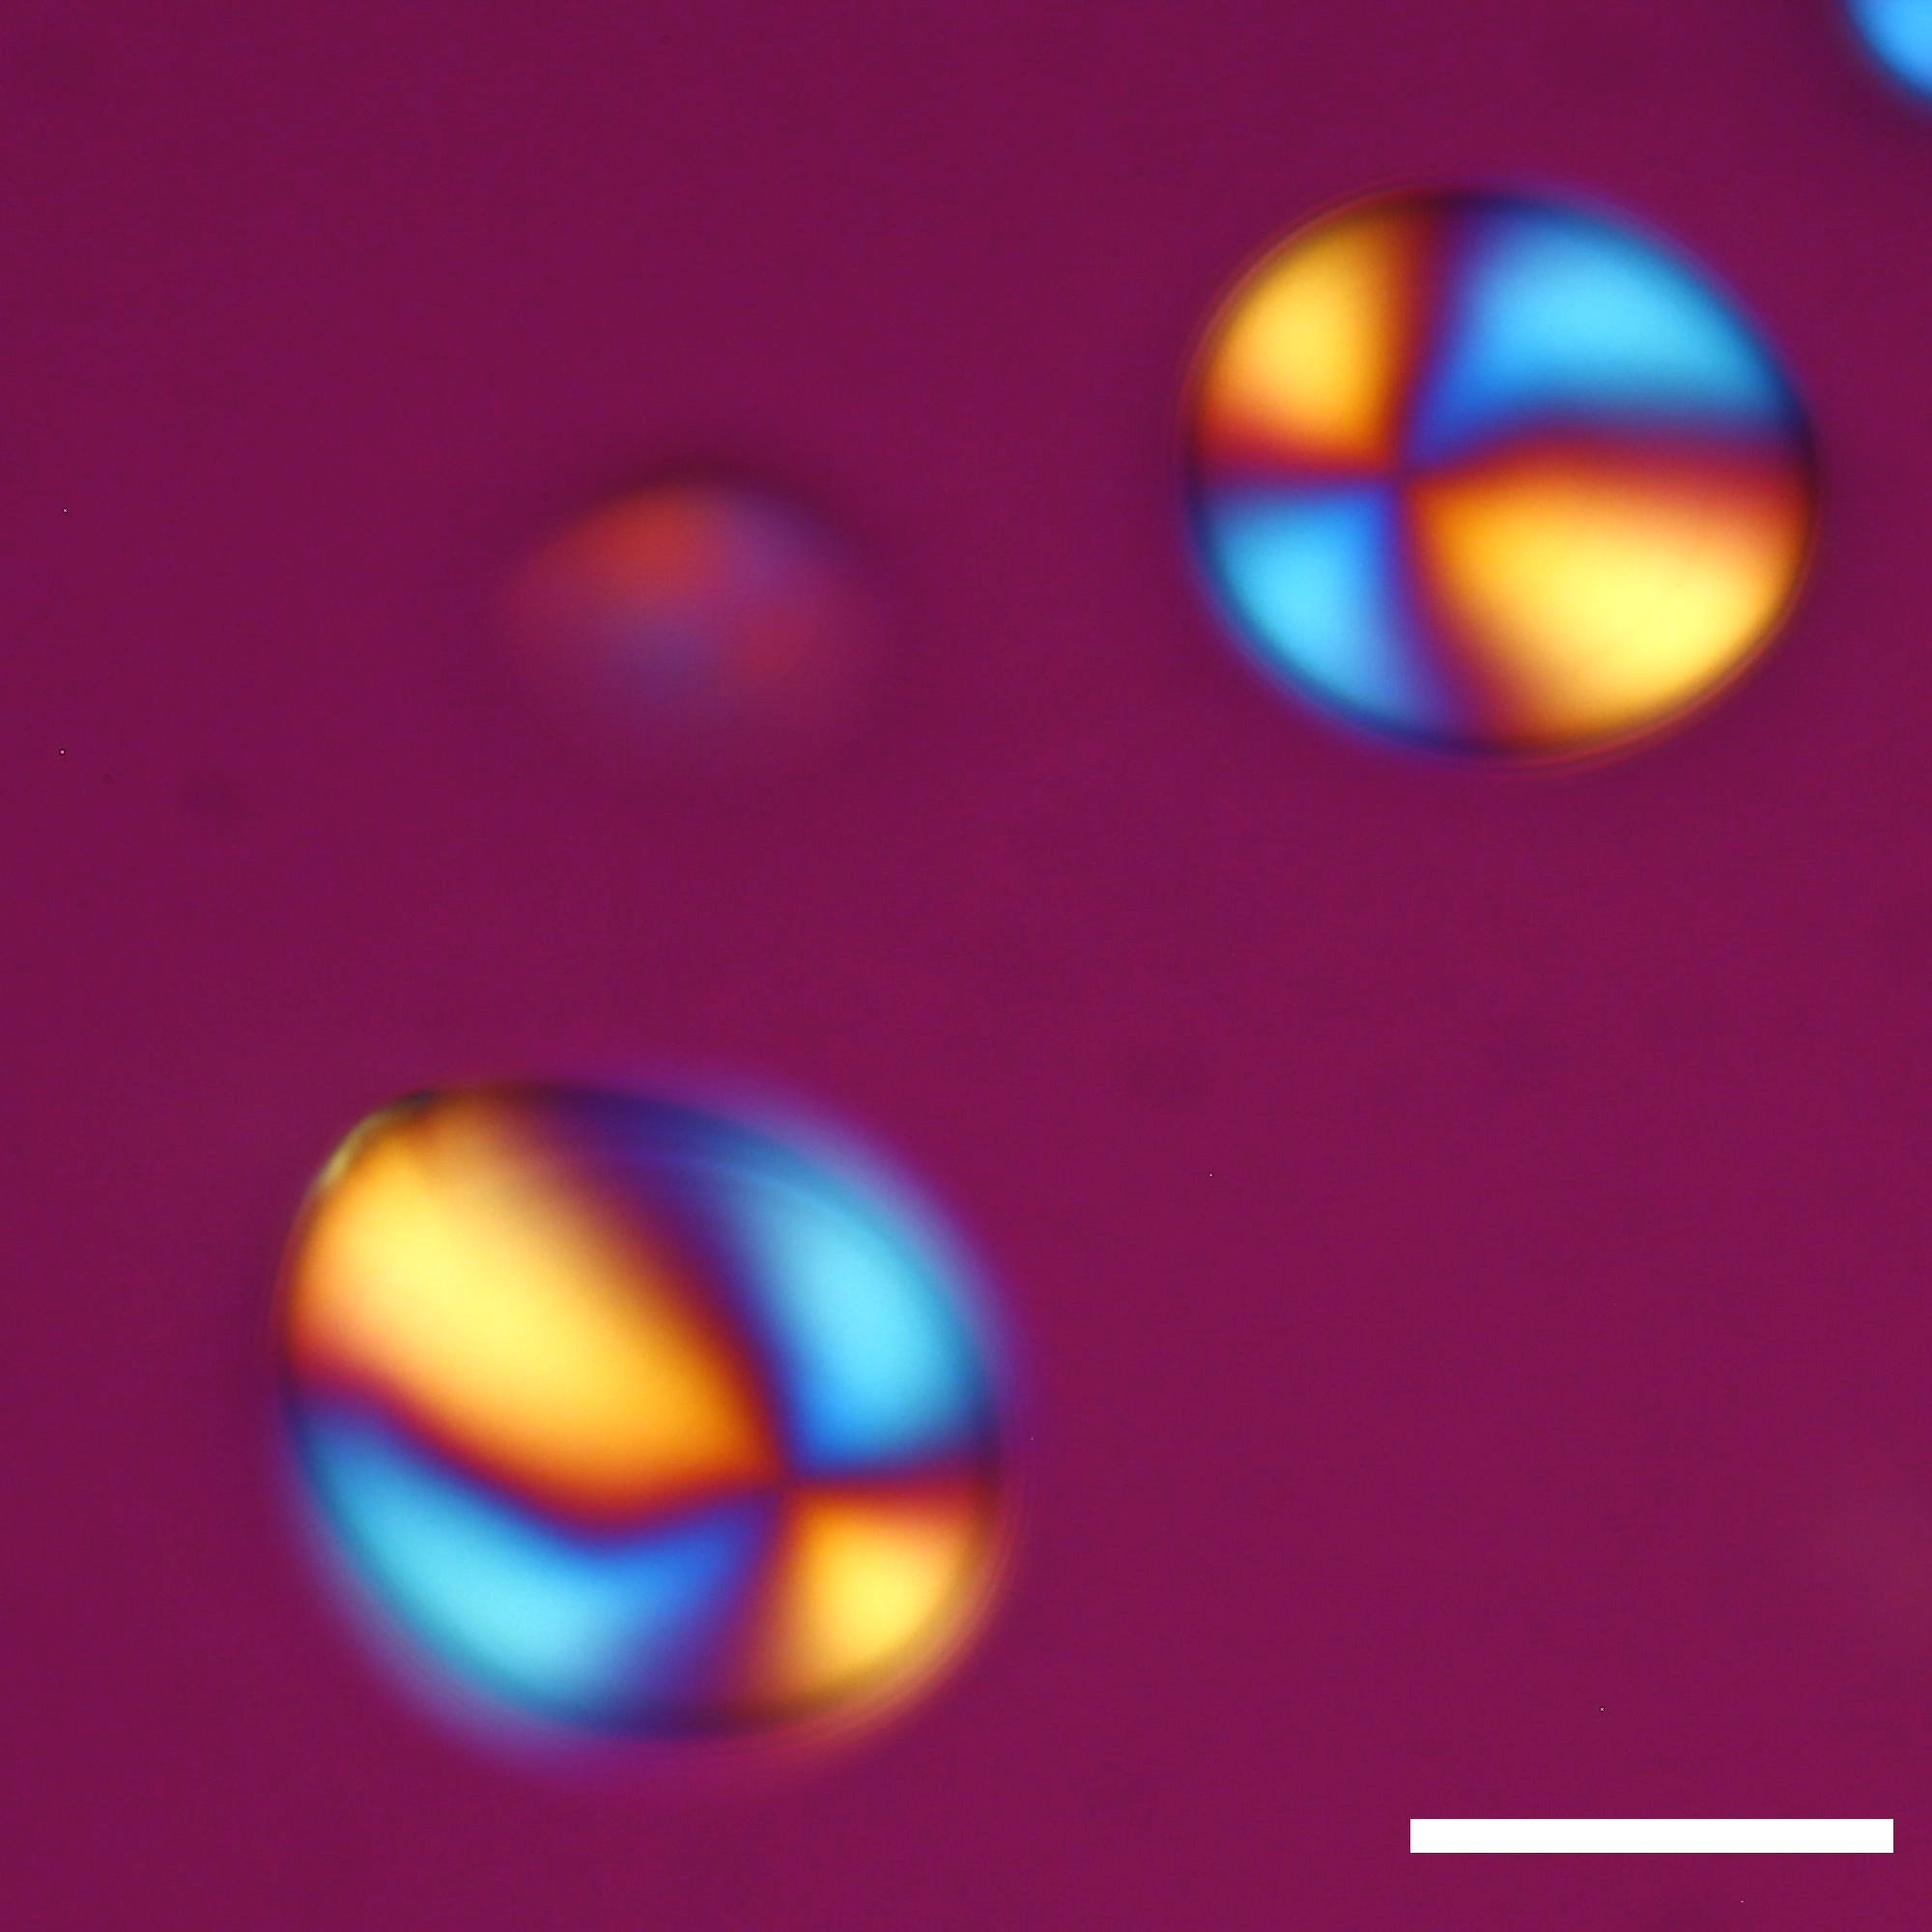
\includegraphics[width=.3\columnwidth]{Exp_2_Microphotography/Figures/48_Starch_Polarization_03_cropped_scale20}}
\caption[Left: brightfield, middle: dic, right: polar.]{Pinewood (top row) and starch (bottom row) specimen under brightfield, DIC, and polarization microscopy. 
Objective lens: Plan Apochromat 63$\times$/1.4 Oil DIC. 
Scalebars are 20 $\mu$m for both specimens.} 
\label{fig:pinestar}
\end{figure}

In Fig.~\ref{pbright}, the brightfield microscopy of pinewood, one can vaguely observe the pits of pinewood that connects one cell's walls to the other. 
Other than generating more contrast, DIC and polarization microscopy allow more fine structures to be observed. 
The birefringent pits (pairs) can be identified more clearly by using either DIC or polarization microscopy (Fig.~\ref{pdic} \&~\ref{ppol}). 
Furthermore, polarization microscopy by using a gypsum platelet red 1$^{st}$ order ($\lambda$ plate) in a crossed position (Fig.~\ref{spol}) allows even more information to be obtained regarding the negative birefringency of pinewood or conversely, positive birefringency for the rod mixed body of starch granules \cite{Lect08}. 
This can be indentified by the orientation of the yellowish-orange and blue color.


%#########################################################################################

%\section{Results and Discussion}
%
%\subsection{Diatoms}
%
%\begin{figure}[h]
%\centering
%\includegraphics[width=.9\columnwidth]{Exp_2_Microphotography/Figures/Merged/Diatomes}
%\caption{Comparison of diatom (\textit{Navicula lyra}) images using brightfield, darkfield, phase contast, and DIC microscopy. Additionally, brightfield microscopy was also conducted using blue and red filters. All images are grey scaled. Fig. A, C, D, E, and F used Plan Neofluar 40$\times$/0.75 Ph2 lens, Fig. B used Achroplan 40$\times$/0.6 Korr lens. Scalebar is 25 $\mu$m.}
%\label{fig:diatomes}
%\end{figure}
%
%Diatoms can have many different structures. Obtaining images of small structures on diatom specimens can demonstrate the influence of light wavelength. Light with longer wavelength (e.g. red light, Fig.~\ref{fig:diatomes}E) does not show minute structures of the diatom well, in comparison to blue light (Fig.~\ref{fig:diatomes}F) which has shorter wavelength. The shorter wavelength of blue light are scattered more strongly by smaller structures (or particles) than the longer wavelength red light, hence the less obvious structures of the diatom when viewed with red light/filter. Both of these lights compose the light for brightfield microscopy (Fig.~\ref{fig:diatomes}A), which gives just as detailed an image as its is for darkfield microscopy (Fig.~\ref{fig:diatomes}B), just inversely illuminated. However, the darkfield images are arguably advantageous in this case due to the fact that since the specimen is unstained, more contrast can be obtained this way in comparison to brightfield microscopy. Other methods to increase contrast were also performed, namely; phase contrast microscopy, whose image in Fig.~\ref{fig:diatomes}C which shows a glowing halo around the specimen, and DIC (Fig.~\ref{fig:diatomes}D) which displays the characteristic pseudo-3D effect.
%
%\subsection{Bloodsmear}
%
%\begin{figure}[h]
%\centering
%\includegraphics[width=.6\columnwidth]{Exp_2_Microphotography/Figures/Merged/Bloodsmear}
%\caption{Bloodsmear specimen under brightfield, darkfield, phase contrast, and DIC microscopy. All images are grey scaled. Fig. A, C, and D used Plan Neofluar 40$\times$/0.75 Ph2 lens, Fig. B used Achroplan 40$\times$/0.6 Korr lens. Scalebar is 10 $\mu$m.}
%\label{fig:blood}
%\end{figure}
%
%In the bloodsmear specimen, all imaging methods (Fig.~\ref{fig:blood}) could help distinguish red blood cells among white blood cells. The darkfield image (Fig.~\ref{fig:blood}B) seems to display this most prominently, other than the fact that the contrast between the background and other cells looks very poor. The phase contrast and DIC (Fig.~\ref{fig:blood}C \&~\ref{fig:blood}D) method allow a better resolution of the cells in comparison to the brightfield (Fig.~\ref{fig:blood}A) and darkfield microscopy. 
%
%\subsection{Blowfly salivary gland}
%
%\begin{figure}[h]
%\centering
%\includegraphics[width=.9\columnwidth]{Exp_2_Microphotography/Figures/Merged/Salgland}
%\caption{Blowfly under fluorescence, brightfield, DIC, and phase contrast microscopy. All images are grey scaled and used Plan Neofluar 40$\times$/0.75 Ph2 lens. Scalebar is 25 $\mu$m.}
%\label{fig:blow}
%\end{figure}
%
%\paragraph{Dye} Are the fluorescent dyes correct? In the dyes slides, red is immunofluorescent
%
%The blowfly salivary gland specimen were stained using three different fluorescent markers, namely; DAPI, Alexa Fluor 488 Phalloidin, and immunofluorescence against FasIII. Each of the markers binds to certain part of the salivary gland. These fluorescent markers can be excited by light with the corresponding excitation wavelength. Immunofluorescence of Fasciclin III on the septate junctions of the cell utilizes green excitation and produces red emission (Fig.~\ref{fig:blow}A). The green emission of Alexa Fluor 488 Phalloidin (Fig.~\ref{fig:blow}B) is excited by blue excitation light, and shows the actin filaments of the cell. The round structures in Fig.~\ref{fig:blow}C shows the nucleus of the cell, to which DAPI binds DNA and emits blue emission. All these organelles would otherwise be invisible in the brightfield microscopy (Fig.~\ref{fig:blow}D). DIC and phase contrast microscopy (Fig.~\ref{fig:blow}E \&~\ref{fig:blow}F respectively) provide a more detailed look into the specimen and reveal structures which would otherwise be invisible in brightfield microscopy without having the necessity to stain the specimen, should the case arise to image in such conditions.
%
%
%\subsection{Pinewood and Starch}
%
%\begin{figure}[h]
%\centering
%\includegraphics[width=.9\columnwidth]{Exp_2_Microphotography/Figures/Merged/Pinestar}
%\caption{Pinewood (top row) and starch (bottom row) specimen under brightfield, DIC, and polarization microscopy. All images are grey scaled except the polarization. All used Plan Apochromat 63$\times$/1.4 Oil DIC lens. Scalebars are 20 $\mu$m for both specimens.}
%\label{fig:pinestar}
%\end{figure}
%
%On Fig.~\ref{fig:pinestar}A, the brightfield microscopy of pinewood, one can vaguely observe the pits of pinewood that connects one call walls to the other. Other than generating more contrast, DIC and polarization microscopy allow more fine structures to be observed. The birefringent pits (pairs) can be identified more clearly by using either DIC or polarization microscopy (Fig.~\ref{fig:pinestar}B \&~\ref{fig:pinestar}C). Furthermore, polarization microscopy by using a gypsum platelet red 1$^{st}$ order ($\lambda$ plate) in a crossed position allows even more information to be obatined regarding the negative birefringency of pinewood or conversely, positive birefringency for the rod mixed body of starch granules (Fig.~\ref{fig:pinestar}F). This can be indentified by the orientation of the yellowish-orange and blue color.

%----------------------------------------------------------------------------------------
%	BIBLIOGRAPHY
%----------------------------------------------------------------------------------------

\renewcommand{\refname}{\spacedlowsmallcaps{References}} % For modifying the bibliography heading

%\bibliographystyle{unsrt}

%\bibliography{sample.bib} % The file containing the bibliography

%----------------------------------------------------------------------------------------
